\documentclass[]{ctexbook}
\usepackage{lmodern}
\usepackage{amssymb,amsmath}
\usepackage{ifxetex,ifluatex}
\usepackage{fixltx2e} % provides \textsubscript
\ifnum 0\ifxetex 1\fi\ifluatex 1\fi=0 % if pdftex
  \usepackage[T1]{fontenc}
  \usepackage[utf8]{inputenc}
\else % if luatex or xelatex
  \ifxetex
    \usepackage{xltxtra,xunicode}
  \else
    \usepackage{fontspec}
  \fi
  \defaultfontfeatures{Ligatures=TeX,Scale=MatchLowercase}
\fi
% use upquote if available, for straight quotes in verbatim environments
\IfFileExists{upquote.sty}{\usepackage{upquote}}{}
% use microtype if available
\IfFileExists{microtype.sty}{%
\usepackage{microtype}
\UseMicrotypeSet[protrusion]{basicmath} % disable protrusion for tt fonts
}{}
\usepackage[unicode=true]{hyperref}
\hypersetup{
            pdftitle={R语言数据分析组队学习},
            pdfauthor={张晋、杨佳达、牧小熊、杨杨卓然、姚昱君},
            pdfborder={0 0 0},
            breaklinks=true}
\urlstyle{same}  % don't use monospace font for urls
\usepackage{listings}
\usepackage{longtable,booktabs}
% Fix footnotes in tables (requires footnote package)
\IfFileExists{footnote.sty}{\usepackage{footnote}\makesavenoteenv{long table}}{}
\usepackage{graphicx,grffile}
\makeatletter
\def\maxwidth{\ifdim\Gin@nat@width>\linewidth\linewidth\else\Gin@nat@width\fi}
\def\maxheight{\ifdim\Gin@nat@height>\textheight\textheight\else\Gin@nat@height\fi}
\makeatother
% Scale images if necessary, so that they will not overflow the page
% margins by default, and it is still possible to overwrite the defaults
% using explicit options in \includegraphics[width, height, ...]{}
\setkeys{Gin}{width=\maxwidth,height=\maxheight,keepaspectratio}
\IfFileExists{parskip.sty}{%
\usepackage{parskip}
}{% else
\setlength{\parindent}{0pt}
\setlength{\parskip}{6pt plus 2pt minus 1pt}
}
\setlength{\emergencystretch}{3em}  % prevent overfull lines
\providecommand{\tightlist}{%
  \setlength{\itemsep}{0pt}\setlength{\parskip}{0pt}}
\setcounter{secnumdepth}{5}
% Redefines (sub)paragraphs to behave more like sections
\ifx\paragraph\undefined\else
\let\oldparagraph\paragraph
\renewcommand{\paragraph}[1]{\oldparagraph{#1}\mbox{}}
\fi
\ifx\subparagraph\undefined\else
\let\oldsubparagraph\subparagraph
\renewcommand{\subparagraph}[1]{\oldsubparagraph{#1}\mbox{}}
\fi

% set default figure placement to htbp
\makeatletter
\def\fps@figure{htbp}
\makeatother

\usepackage{ctex}

\lstset{
  breaklines=true
}

\newcommand{\passthrough}[1]{#1}
\usepackage{booktabs}
\usepackage{longtable}
\usepackage{array}
\usepackage{multirow}
\usepackage{wrapfig}
\usepackage{float}
\usepackage{colortbl}
\usepackage{pdflscape}
\usepackage{tabu}
\usepackage{threeparttable}
\usepackage{threeparttablex}
\usepackage[normalem]{ulem}
\usepackage{makecell}
\usepackage{xcolor}

\title{R语言数据分析组队学习}
\author{张晋、杨佳达、牧小熊、杨杨卓然、姚昱君}
\date{}

\begin{document}
\maketitle

{
\setcounter{tocdepth}{2}
\tableofcontents
}
\hypertarget{welcome}{%
\section*{欢迎!}\label{welcome}}


欢迎来到由DataWhale主办的R语言数据分析组队学习课程。

\hypertarget{ux8d21ux732eux8005ux4fe1ux606f}{%
\subsection*{贡献者信息}\label{ux8d21ux732eux8005ux4fe1ux606f}}


\begin{tabular}{l|l|l}
\hline
姓名 & 介绍 & 个人主页\\
\hline
张晋 & Datawhale成员,算法竞赛爱好者 & https://blog.csdn.net/weixin\_44585839/\\
\hline
杨佳达 & 数据挖掘师,Datawhale成员,目前在国内某第三方数据服务公司做数据分析挖掘及数据产品 & https://github.com/yangjiada\\
\hline
牧小熊 & 华中农业大学研究生,Datawhale成员,Datawhale优秀原创作者 & https://www.zhihu.com/people/muxiaoxiong\\
\hline
杨杨卓然 & 混吃等死统计休学穷酸书生 & https://yangzhuoranyang.com\\
\hline
姚昱君 & 悉尼大学,Datawhale成员 & https://blog.csdn.net/Yao\_June\\
\hline
\end{tabular}

\hypertarget{ux8bfeux7a0bux7b80ux4ecb}{%
\subsection*{课程简介}\label{ux8bfeux7a0bux7b80ux4ecb}}


\begin{itemize}
\tightlist
\item
  课程设计成员:\textbf{张晋}、杨佳达、牧小熊、杨杨卓然、姚昱君
\item
  学习周期:16天,每天平均花费时间1小时-3小时不等,根据个人学习接受能力强弱有所浮动。
\item
  学习形式:理论学习 + 练习
\item
  人群定位:对数据科学有基本了解,希望学习R语言的同学。
\item
  先修内容:无
\item
  难度系数:⭐⭐
\end{itemize}

\hypertarget{ux8bfeux7a0bux5927ux7eb2}{%
\subsection*{课程大纲}\label{ux8bfeux7a0bux5927ux7eb2}}


\textbf{Task00:熟悉规则与R语言入门(1天)}

\begin{itemize}
\tightlist
\item
  安装
\item
  环境配置
\end{itemize}

\textbf{Task01 数据结构与数据集 (3天)}

\begin{itemize}
\tightlist
\item
  编码基础
\item
  数据类型
\item
  特殊数据类型
\item
  table like 数据类型
\item
  加载数据 (csv, rds, excel, Rdata)
\item
  实例
\end{itemize}

\textbf{Task02 数据清洗与准备 (3天)}

\begin{itemize}
\tightlist
\item
  重复值处理
\item
  缺失值识别与处理
\item
  异常值识别与处理
\item
  特征处理
\item
  规范化与偏态数据
\end{itemize}

\textbf{Task03 基本统计分析 (3天)}

\begin{itemize}
\tightlist
\item
  多种方法获取描述性统计量
\item
  分组计算描述性统计
\item
  频数表和列联表
\item
  相关
\item
  方差分析
\end{itemize}

\textbf{Task04 数据可视化(3天)}

\begin{itemize}
\tightlist
\item
  ggplot2包介绍
\item
  散点图
\item
  直方图
\item
  柱状图
\item
  饼状图
\item
  折线图
\item
  ggplot2扩展包主题
\end{itemize}

\textbf{Task05 模型(3天)}

\begin{itemize}
\tightlist
\item
  回归模型
\item
  分类模型
\end{itemize}

\hypertarget{ux5173ux4e8e-datawhale}{%
\subsection*{关于 Datawhale}\label{ux5173ux4e8e-datawhale}}


Datawhale 是一个专注于数据科学与AI领域的开源组织,汇集了众多领域院校和知名企业的优秀学习者,聚合了一群有开源精神和探索精神的团队成员。Datawhale 以 ``For the learner,和学习者一起成长'' 为愿景,鼓励真实地展现自我、开放包容、互信互助、敢于试错和勇于担当。同时 Datawhale 用开源的理念去探索开源内容、开源学习和开源方案,赋能人才培养,助力人才成长,建立起人与人,人与知识,人与企业和人与未来的联结。 本次数据挖掘路径学习,专题知识将在天池分享,详情可关注 Datawhale:


\includegraphics[width=3.58in]{image/logo}

\hypertarget{part-ux51c6ux5907ux5de5ux4f5c}{%
\part{准备工作}\label{part-ux51c6ux5907ux5de5ux4f5c}}

\hypertarget{task-00}{%
\section*{熟悉规则与R语言入门}\label{task-00}}


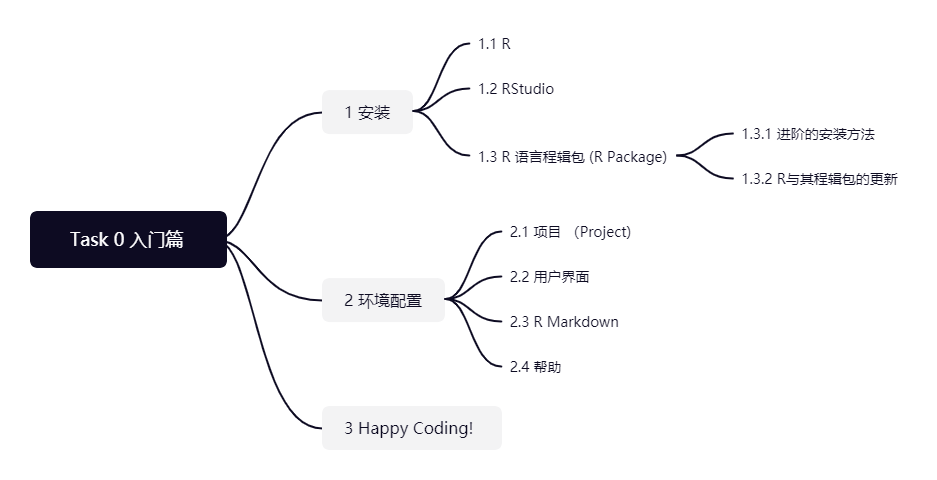
\includegraphics[width=1\textwidth,height=\textheight]{./image/task00_intro_structure.jpg}

\hypertarget{ux5b89ux88c5}{%
\subsection{安装}\label{ux5b89ux88c5}}

\hypertarget{r}{%
\subsubsection{R}\label{r}}

\begin{itemize}
\tightlist
\item
  R 语言是一门用于统计计算与绘图的编程语言和开源软件(\href{https://www.r-project.org/}{The R Foundation})。
\item
  R 语言是当今应用最多的统计软件之一。
\item
  截止到这份文档编写时,在 CRAN (\href{https://cran.r-project.org/}{the Comprehensive R Archive Network}) 上总共发行了17955个R语言程辑包。
\item
  除了 CRAN 以外,R 语言的程辑包作者也在其他线上代码托管与研发协作平台发布了数不尽的作品。这样的平台包括 \href{https://github.com/}{GitHub}、\href{https://about.gitlab.com}{GitLab}、\href{https://gitee.com/}{Gitee} 等。
\end{itemize}

你可以从 CRAN 的网站上下载 R:\url{https://cloud.r-project.org/}。
你也可以在\href{https://cran.r-project.org/mirrors.html}{这里}选择任意一个镜像网站来下载 R.

\hypertarget{rstudio}{%
\subsubsection{RStudio}\label{rstudio}}

\href{https://rstudio.com/products/rstudio/}{RStudio} 是针对 R 语言设计的集成开发环境。如果没有 RStudio 的话,R 本身只提供一个简单的文本编辑器。如果把R语言本身比喻成飞机的话,那么 RStudio 便是飞机场:你不需要它就可以飞,但是有了它会极大增加效率。它包括一个控制台、语法突出显示的编辑器、直接执行代码的支持,以及用于绘图、历史记录、调试和工作区管理的工具。

你可以从其官网下载开源版本:\url{https://rstudio.com/products/rstudio/}

在本文档中,我们会介绍 RStudio 的用户界面和部分功能,帮助你尽快上手使用 RStudio 的数据分析。

\hypertarget{rux8bedux8a00ux7a0bux8f91ux5305r-package}{%
\subsubsection{R语言程辑包(R Package)}\label{rux8bedux8a00ux7a0bux8f91ux5305r-package}}

R 语言程辑包是 R 语言必不可少的部分。R语言能有他今天在统计学里的位置正是归功于其程辑包在统计计算方面的发展。一个程辑包为用户提供函数(function)、数据(data)或者插件(addins)。除了 R 本身自带的基础程辑包(base、utils、stats等)以外,你还可以用以下代码来从 CRAN 上下载并安装额外的程辑包:

\begin{lstlisting}[language=R]
install.packages("tidyverse")
\end{lstlisting}

我们将会在这次组队学习中多次用到\passthrough{\lstinline!tidyverse!}。它其实是一系列程辑包的组合,主要提供数据清洗与处理的工具。

\hypertarget{ux8fdbux9636ux7684ux5b89ux88c5ux65b9ux6cd5}{%
\paragraph{进阶的安装方法}\label{ux8fdbux9636ux7684ux5b89ux88c5ux65b9ux6cd5}}

当你应用 R 语言的能力到一定阶段之后,你会发现自己需要安装不在 CRAN 上发布的程辑包,或者你需要最新版本的程辑包( CRAN 上的包为了保证代码的可靠性,发布前需要经过一系列的检查与测试,这就导致 CRAN 上的版本往往不是最新的开发版本)。以安装 GitHub 上发布的程辑包为例,你可以使用以下代码:

\begin{lstlisting}[language=R]
# 安装 remotes 包
install.packages("remotes")
# 使用 remotes 从 GitHub 上安装 username 名下的 repo 包
remotes::install_github("username/repo")
\end{lstlisting}

我们需要先安装 \passthrough{\lstinline!remotes!} 包,并使用其中的 \passthrough{\lstinline!install\_github!} 函数来完成操作。注意这里是从源代码安装,在本地编译。Windows 用户需要使用 Rtools 作为背后的编译工具。关于 Rtools 的安装信息见 \url{https://cran.r-project.org/bin/windows/Rtools/}

\hypertarget{rux4e0eux5176ux7a0bux8f91ux5305ux7684ux66f4ux65b0}{%
\paragraph{R与其程辑包的更新}\label{rux4e0eux5176ux7a0bux8f91ux5305ux7684ux66f4ux65b0}}

在本文档编写之时,R 语言已更新到版本R version 4.1.0 (2021-05-18)。当新的版本发布时,你可以使用 \passthrough{\lstinline!installr!} 包中的 \passthrough{\lstinline!installr!} 函数来完成R的更新(你当然也可以手动下载更新,如果不嫌麻烦的话)。代码如下:

\begin{lstlisting}[language=R]
# 安装 installr 包
install.packages(installr)
# 更新 R
installr::installr()
\end{lstlisting}

根据对话窗口中的提示完成整个安装过程即可。

你也可以使用以下代码来更新R的程辑包:

\begin{lstlisting}[language=R]
# 手动确认是否将各个更新到最新版本,或者
update.packages()
# 更新所有包到最新版本
update.packages(ask = FALSE)
\end{lstlisting}

\hypertarget{ux73afux5883ux914dux7f6e}{%
\subsection{环境配置}\label{ux73afux5883ux914dux7f6e}}

\hypertarget{ux9879ux76eeproject}{%
\subsubsection{项目(Project)}\label{ux9879ux76eeproject}}

在RStudio中一个项目(Project)本质上是一个把项目相关的文件储存在一个地方的文件夹。如果使用项目相关的功能的话,你不需要担心使用的文件是否在当前的工作目录(Working Directory)。 项目功能提供了一个将不同目的的文件分隔开的方式,同时自动保存上次相应的工作进度。

\hypertarget{ux7ec3ux4e60}{%
\paragraph*{练习}\label{ux7ec3ux4e60}}
\addcontentsline{toc}{paragraph}{练习}

为这次组队学习建立一个新的项目。

每次进行组队学习的时候,不要忘记去打开这个项目。在结束工作退出R,或者切换到另一个项目的时候,为了下次打开 RStudio 的时候有一个干净的工作环境,建议不去保存``工作空间镜像'' (Workspace image,即在当前进程中加载的数据、函数)。

创建新的项目,可以在下拉菜单 \textbf{File} (或者RStudio界面的右上角)找到 \textbf{New Project} 选项。在弹出的对话框中,如果你想创建一个新的文件夹作为项目文件夹,选择 \textbf{New Directory} ;如果你想用一个已经存在的文件夹作为项目文件夹,选择 \textbf{Existing Directory} 。

\begin{figure}
\centering
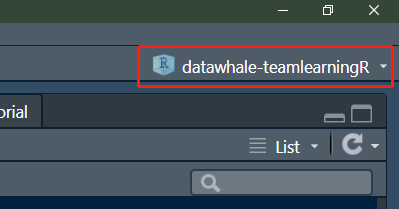
\includegraphics{./image/task00_project.png}
\caption[RStudio 界面右上角的项目设置]{RStudio 界面右上角的项目设置\footnotemark{}}
\end{figure}
\footnotetext{小提示:如果想要改变 RStudio 的主题颜色,可以通过 \textbf{Tools} \textgreater\textgreater{} \textbf{Global Options..} \textgreater\textgreater{} \textbf{Appearance}}

\hypertarget{ux7528ux6237ux754cux9762}{%
\subsubsection{用户界面}\label{ux7528ux6237ux754cux9762}}

接下来让我们关注一下 RStudio 用户界面里的各种面板和标签。在这一部分有四个基础面板值得注意。

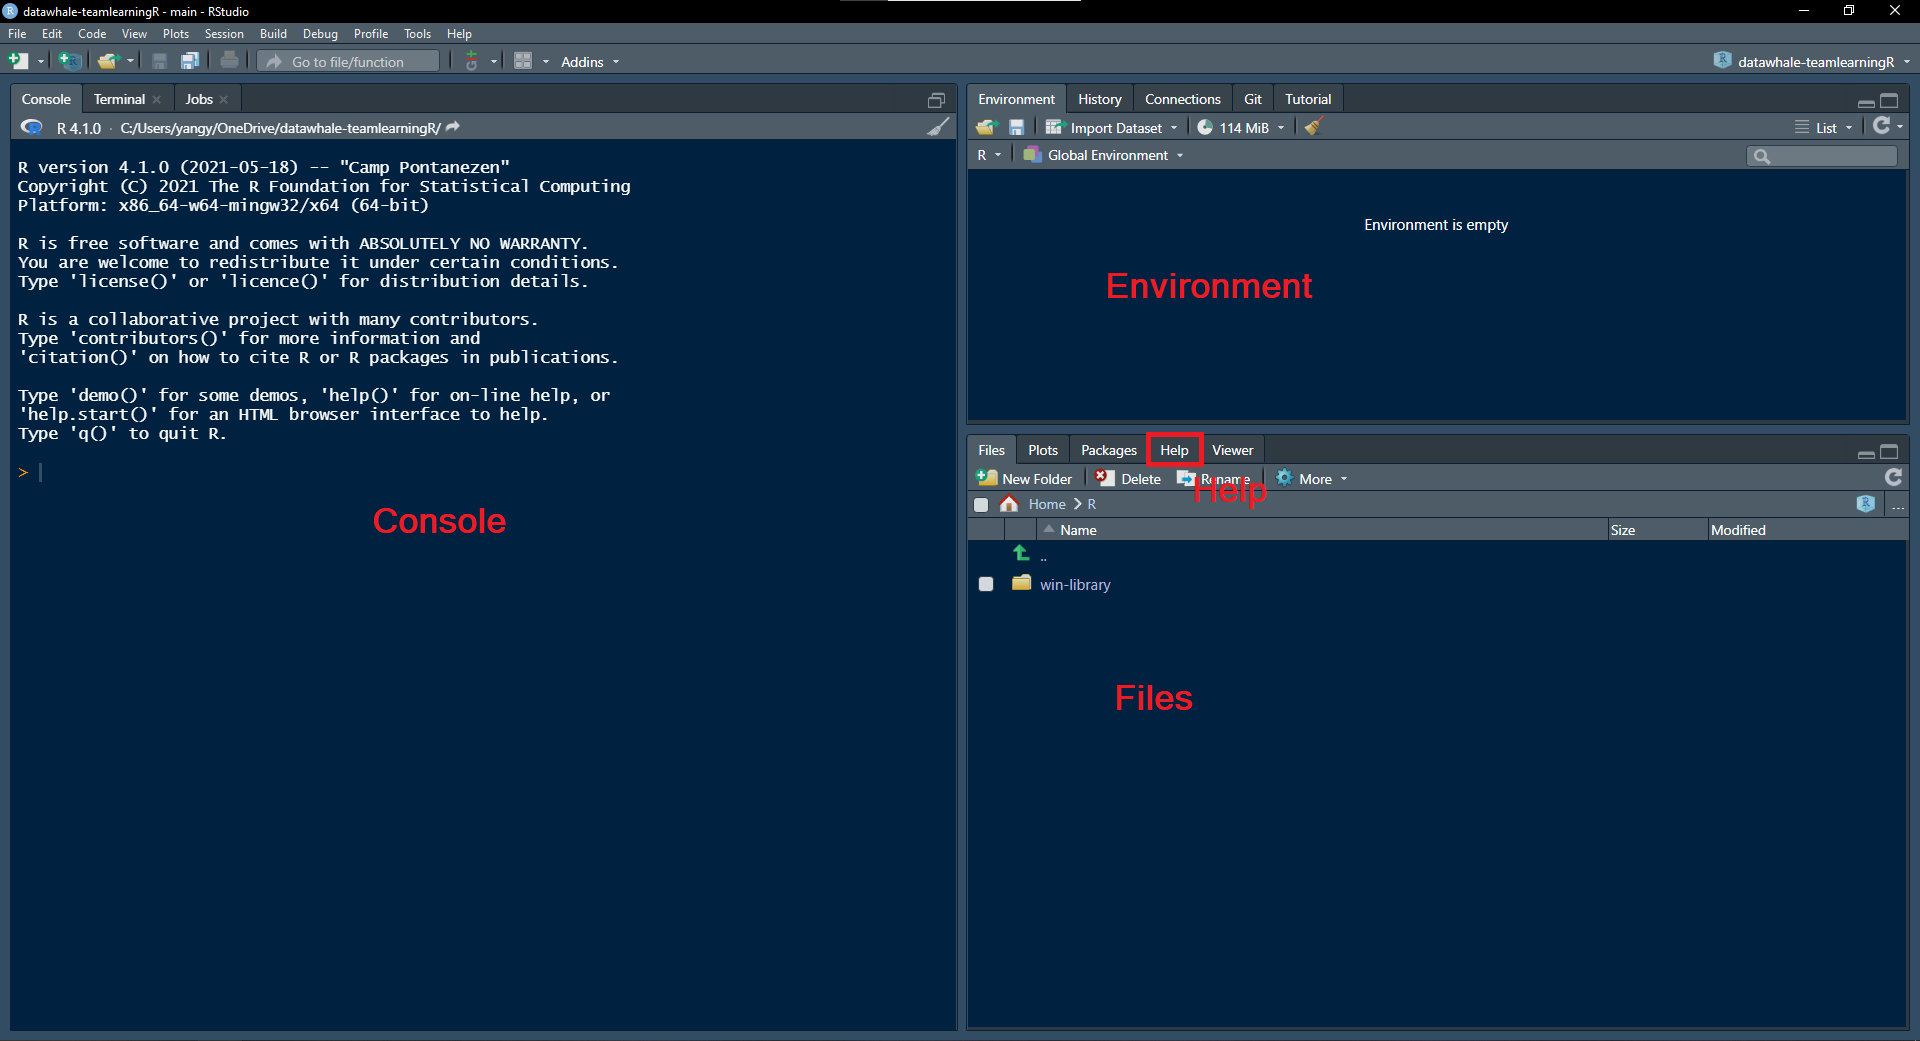
\includegraphics{./image/Rstudio.png}

\begin{itemize}
\tightlist
\item
  \textbf{Console} 控制台位于界面左侧。你可以在这里运行命令、浏览输出结果。
\item
  \textbf{Environment} 位于界面右上方。环境面板会总结出当前加载的数据、定义的函数等。现在在你看来可能是空的,因为我们还没有做任何事情。
\item
  \textbf{Files} 位于界面右下方。文件面板展示当前文件夹的信息。
\item
  \textbf{Help} 帮助面板也位于界面右下方。在这里你可以找到相应数据或者函数的帮助信息。
\end{itemize}

\hypertarget{r-markdown}{%
\subsubsection{R Markdown}\label{r-markdown}}

你可以控制台(Concole)直接运行命令,但是这样跑出来的指令不会被保存下来。一般来说,我们更建议将命令写在叫做 R script 的脚本中,或者写在一个叫做 R Markdown 的文件中。

\hypertarget{ux7ec3ux4e60-1}{%
\paragraph*{练习}\label{ux7ec3ux4e60-1}}
\addcontentsline{toc}{paragraph}{练习}

创建一个脚本 R script.

\begin{itemize}
\tightlist
\item
  \textbf{File} \textgreater\textgreater{} \textbf{New File} \textgreater\textgreater{} \textbf{R Script}
\end{itemize}

\hypertarget{ux7ec3ux4e60-2}{%
\paragraph*{练习}\label{ux7ec3ux4e60-2}}
\addcontentsline{toc}{paragraph}{练习}

创建一个 R Markdown 文件。

\begin{itemize}
\tightlist
\item
  \textbf{File} \textgreater\textgreater{} \textbf{New File} \textgreater\textgreater{} \textbf{R Markdown..}
\end{itemize}

在脚本或者 R Markdown 的界面中,界面上方可以找到一个运行所有代码的按键。

一个 R Markdown 文件是一个可以将代码与 \emph{markdown} 标准文本(一种纯文本的格式语法)结合在一起的文本文档。使用 R Markdown 文件可以很容易地生成 pdf 文件或者 html 文件,其中不止包含了你的文本,还有代码以及运行代码所生成的结果。点击界面上方的 \textbf{Knit} 按键\footnote{如果你想要生成 pdf 文件,你需要安装 \href{https://www.latex-project.org/}{LaTeX}。可以看看很好地兼容了 R 的\href{https://yihui.org/tinytex/}{TinyTex}。}即可。再也不需要复制粘贴、屏幕截图输出结果到 Word 了。R Markdown 文档的一个主要优势是可复现。只要有了同样的代码和数据,你可以获得与其他人一模一样的结果,只要生成文档就可以了。

在 R Markdown 文件里写代码,需要使用特定的代码块(code chunks)来告诉 R Markdown 这部分是需要运行的代码而不只是文本。\footnote{R Markdown 的更多语法可以看看 \href{https://rstudio.com/wp-content/uploads/2016/03/rmarkdown-cheatsheet-2.0.pdf}{R Markdown cheatsheet}。}

\begin{lstlisting}
```{r}

# 在这里写你的代码
# 使用三个反引号和 {r} 起始,三个反引号结束来构建代码块
# 在代码块里使用井号 # 写评论(纯文本) 

```
\end{lstlisting}

\hypertarget{ux5e2eux52a9}{%
\subsubsection{帮助}\label{ux5e2eux52a9}}

R 能够发展到其今天的地位,很大的一个因素是他提供了相对详细的帮助文档,对初学者相对友好。一个相对完整的 R 包最低标准便是有函数的帮助文档。需要查看一个具体函数或者数据的帮助时可以用 \passthrough{\lstinline!?fun!}(等同于 \passthrough{\lstinline!help(fun)!}),该函数 \passthrough{\lstinline!fun!} 的帮助文档便会出现在之前提到过的帮助面板里。这个是已经知道需要什么函数了之后查找具体函数的用法的方式,如果你不记得具体的函数名字,可以使用两个问号加关键字来搜索:\passthrough{\lstinline!??keyword!}。

其次R包会有一个或多个 vignette。vignette 文档的目的主要是当使用者不知道用什么函数,对这个包不了解的时候提供一份入门简介一样的东西,一般会对常用的函数做出说明和演示,以及一些理论的阐述。这个包如果是哪一篇论文的副产品,vignette 甚至有可能是这篇论文。根据包的大小不同,vignette 的数量也不一样。如果是针对于一个问题写出的精炼的小包的话会只有一个 vignette 。如果包的用途比较广泛或者作者想说的话比较多,会针对每个问题有一个单独的 vignette。浏览所有已安装的 vignette 用 \passthrough{\lstinline!browseVignettes()!} ,查看具体包的用\passthrough{\lstinline!browseVignettes("packagename")!}。以上两个是通过 CRAN 发行的包的标配。

如果这个包没有在 CRAN 上发行,只在 GitHub 上,或者 GitHub 上有开发版本的话,一般会有一个 \passthrough{\lstinline!README.md!} 的文档。这个文档相对于 vignette 来说更加简短,一般都只写明如何安装,以及最主要的命令的演示,没有太多的说明。文档最后有可能会说明这个包用的是什么许可证。如果有这么一个文件的话,就可以很快速的知道这个包最主要的命令是什么。这个文档就需要到相对应的R包的资源库搜索了。

\begin{lstlisting}[language=R]
## 总结
# 查看具体函数的帮助文档
?fun
help(fun)
# 在帮助文档中搜索关键词
??keyword
# 浏览所有已安装的vignette
browseVignettes()
# 查看具体包的vignette
browseVignettes("packagename")
\end{lstlisting}

\hypertarget{happy-coding}{%
\subsection{Happy Coding!}\label{happy-coding}}

这次的R语言数据分析组队学习的入门篇便到这里了。接下里请移步组队学习的正篇第一部分:数据结构与数据集。

玩得开心!

\hypertarget{ux672cux7ae0ux4f5cux8005}{%
\subsection*{本章作者}\label{ux672cux7ae0ux4f5cux8005}}


\textbf{Fin}

\begin{quote}
\url{https://yangzhuoranyang.com}
\end{quote}

\hypertarget{ux5173ux4e8edatawhale}{%
\subsection*{关于Datawhale}\label{ux5173ux4e8edatawhale}}


Datawhale 是一个专注于数据科学与AI领域的开源组织,汇集了众多领域院校和知名企业的优秀学习者,聚合了一群有开源精神和探索精神的团队成员。Datawhale 以``for the learner,和学习者一起成长''为愿景,鼓励真实地展现自我、开放包容、互信互助、敢于试错和勇于担当。同时 Datawhale 用开源的理念去探索开源内容、开源学习和开源方案,赋能人才培养,助力人才成长,建立起人与人,人与知识,人与企业和人与未来的联结。 本次数据挖掘路径学习,专题知识将在天池分享,详情可关注 Datawhale:


\includegraphics[width=3.58in]{image/logo}

\hypertarget{part-ux5f00ux59cbux5e72ux6d3b}{%
\part{开始干活}\label{part-ux5f00ux59cbux5e72ux6d3b}}

\hypertarget{task-01}{%
\section{数据结构与数据集}\label{task-01}}

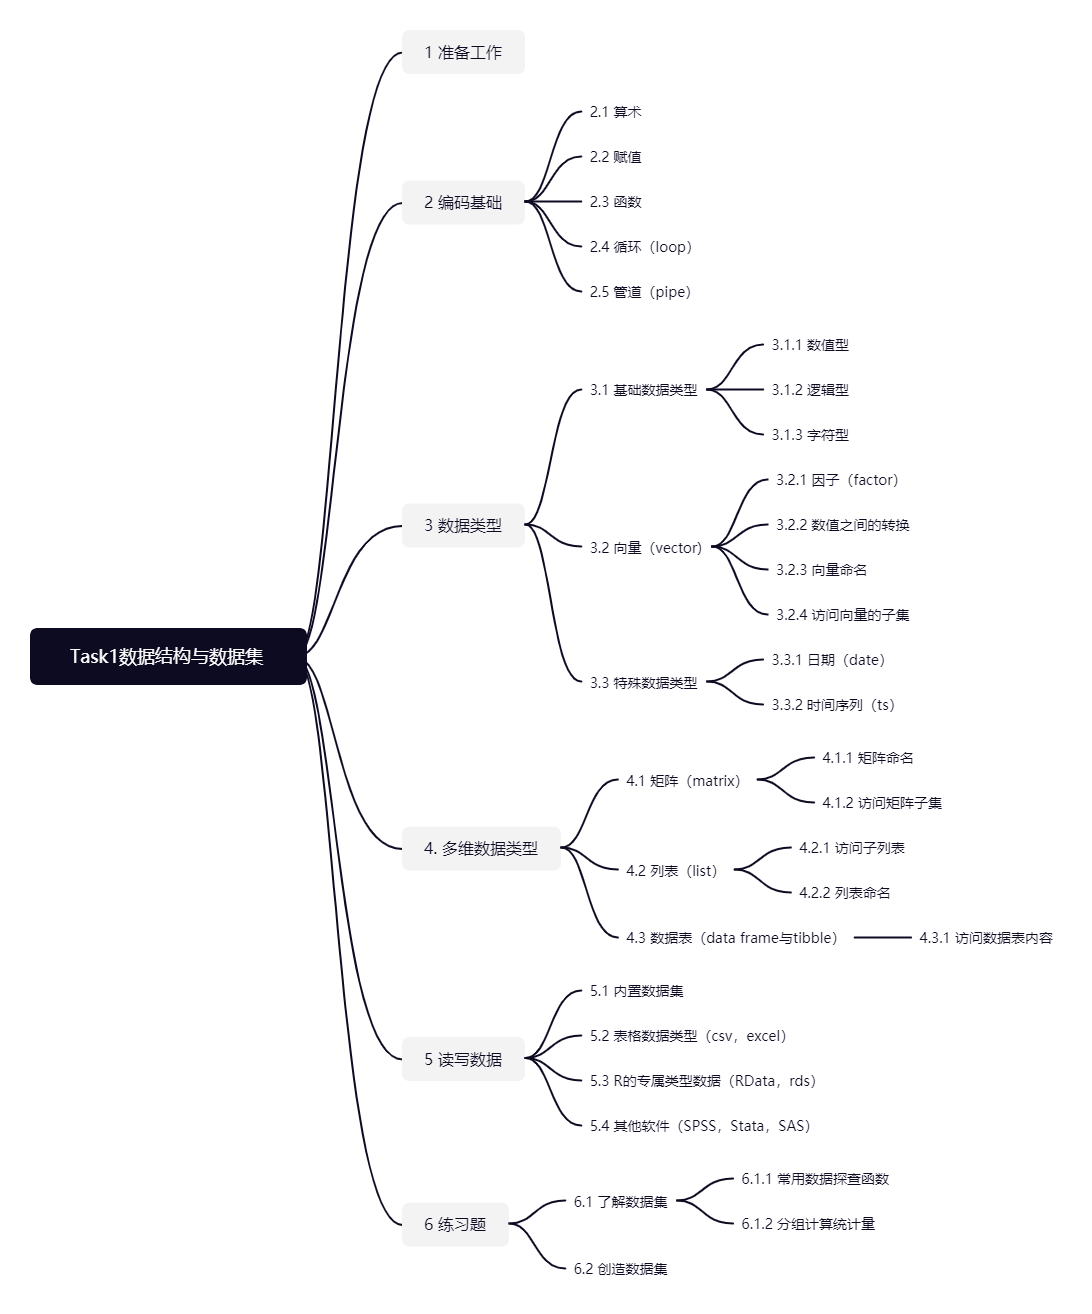
\includegraphics[width=1\textwidth,height=\textheight]{./image/task01_data_structure.jpg}

\hypertarget{ux51c6ux5907ux5de5ux4f5c}{%
\subsection{准备工作}\label{ux51c6ux5907ux5de5ux4f5c}}

这节组队学习的目的主要是帮助你上手R的基本编程逻辑,了解一些R编程的基本概念,包括各个数据类型和数据集的读取与保存。

在开始我们的学习之前,不要忘记在 R Studio 中切换到组队学习专属的项目,打开一个 R script 文件或者 R Markdown 文件(详见入门篇)。

\hypertarget{ux7f16ux7801ux57faux7840}{%
\subsection{编码基础}\label{ux7f16ux7801ux57faux7840}}

首先我们来了解一些基本的编码操作。在 R Studio 中想要运行代码可以在控制台 Console 中键入代码后点击回车。这样运行的代码会被保存在当前项目的 \passthrough{\lstinline!.Rhistory!} 文件中,也可以在 R Studio 界面右上角的 History 面板中找到,但是不会被明确地保存下来作为一个脚本文件。一般只有在我们想要运行一些简单的指令或者计算的时候才会采取这种方式。更常见的是将代码写在脚本文件中,选中相应的代码后点击界面上方的Run或者快捷键(\passthrough{\lstinline!Ctrl!} + \passthrough{\lstinline!Enter!})来运行。

\hypertarget{ux7b97ux672f}{%
\subsubsection{算术}\label{ux7b97ux672f}}

你可以直接运行计算命令。计算符号包括加\passthrough{\lstinline!+!}、减\passthrough{\lstinline!-!}、乘\passthrough{\lstinline!*!}、除\passthrough{\lstinline!/!}、求幂\passthrough{\lstinline!\^!}以及求余数\passthrough{\lstinline!\%\%!}等。值得一提的是开平方根有他自己单独的函数\passthrough{\lstinline!sqrt!}。

\begin{lstlisting}[language=R]
1 + 1
\end{lstlisting}

\begin{lstlisting}
## [1] 2
\end{lstlisting}

\begin{lstlisting}[language=R]
1 - 1
\end{lstlisting}

\begin{lstlisting}
## [1] 0
\end{lstlisting}

\begin{lstlisting}[language=R]
1 * 2
\end{lstlisting}

\begin{lstlisting}
## [1] 2
\end{lstlisting}

\begin{lstlisting}[language=R]
1 / 2
\end{lstlisting}

\begin{lstlisting}
## [1] 0.5
\end{lstlisting}

\begin{lstlisting}[language=R]
3 %% 2
\end{lstlisting}

\begin{lstlisting}
## [1] 1
\end{lstlisting}

\begin{lstlisting}[language=R]
2^(1 / 2)
\end{lstlisting}

\begin{lstlisting}
## [1] 1.414214
\end{lstlisting}

\begin{lstlisting}[language=R]
sqrt(2)
\end{lstlisting}

\begin{lstlisting}
## [1] 1.414214
\end{lstlisting}

\hypertarget{ux8d4bux503c}{%
\subsubsection{赋值}\label{ux8d4bux503c}}

在 R 里,我们可以为一个``东西''取一个名字,这个``东西''可以是一个值、一个向量、或者一个函数等,这样我们就可以之后再获取存储在这个名字下面的信息。

\begin{lstlisting}[language=R]
# 将数字42赋予名叫x的变量
x <- 42
# 在R中运行一个物体的名字
# R将会打印出(print)该物体的值
x
\end{lstlisting}

\begin{lstlisting}
## [1] 42
\end{lstlisting}

在 R 中基础赋值的符号有三种:

\begin{enumerate}
\def\labelenumi{\arabic{enumi}.}
\tightlist
\item
  一个向左的箭头\passthrough{\lstinline!<-!}表示将箭头右方的值取名叫做箭头左侧的名字,或者将箭头右侧的值存储在箭头左侧的名字里;
\item
  一个向右的箭头\passthrough{\lstinline!->!}表示将箭头左侧的值储存在箭头右侧的名字里;
\item
  一个等号\passthrough{\lstinline!=!}表示将箭头右侧的值存储在箭头左侧的名字里(同1)。
\end{enumerate}

在早期的键盘中有一个单独的按键就是向左的箭头,虽然后来的键盘不再设立这个按键,但是使用箭头的编程习惯流传了下来。赋值符号的选择取决于个人习惯,但是我们大多数情况下都推荐使用箭头(尤其是向左的箭头)作为赋值的符号。这是R语言于其他语言不同的地方,有以下原因:

\begin{enumerate}
\def\labelenumi{\arabic{enumi}.}
\tightlist
\item
  箭头明确了赋值方向,这是等号做不到的;
\item
  等号用在顶层环境中的时候是赋值,用在函数中则是设参(或者叫做在函数层面赋值)。这种二义性不小心区分则可能会引发错误。而等号即使用在函数中也是赋值;
\item
  箭头可以做到多次赋值(\passthrough{\lstinline!a <- b <- 42!})甚至是不同方向上多次赋值(\passthrough{\lstinline!a <- 42 -> b!})(尽量避免!);
\item
  虽然这次组队学习中不会学到,但是更高级的赋值工具包括 \passthrough{\lstinline!<<-!} 和 \passthrough{\lstinline!->>!} 对应向左或向右的箭头;
\item
  同时使用\passthrough{\lstinline!=!}与\passthrough{\lstinline!==!}(判断是否相等)会降低可读性(\passthrough{\lstinline!a <- 1 == 2!} vs \passthrough{\lstinline!a = 1 == 2!})。
\end{enumerate}

总结,\textbf{凡是赋值都用\passthrough{\lstinline!<-!}},凡是设参(之后会说到)都用\passthrough{\lstinline!=!}。

在 R Studio 中可以使用快捷键\passthrough{\lstinline!Alt!} + \passthrough{\lstinline!-!}来输入\passthrough{\lstinline!<-!},这样就不用每次都点两次键啦。这样还有一个好处,就是 R Studio 会自动识别当前的输入语言,从而选择最佳的赋值符号。大多数情况下这也就是说他会输入R的\passthrough{\lstinline!<-!},如果你在 R Studio 里用 Python 的话就会自动变成\passthrough{\lstinline!=!}啦。

原来作用于单纯数字上的算术运算现在即可用变量名称代替具体的数值。

\begin{lstlisting}[language=R]
y <- 21
x + y
\end{lstlisting}

\begin{lstlisting}
## [1] 63
\end{lstlisting}

\begin{lstlisting}[language=R]
x <- x + y
\end{lstlisting}

\hypertarget{ux51fdux6570}{%
\subsubsection{函数}\label{ux51fdux6570}}

R是一个非纯函数式编程(Functional Programming)的语言,与你平时可能所熟悉的面向对象程序设计(Object-Oriented Programming)的编程语言(比如 Python)不一样。这意味着在R中,相对于以类(Class)与对象(Object)的思路思考问题,我们要更多地定义函数(Function)以及考虑函数的输入与输出来进行运算。(如果你不知道我在这里说什么,请忽略这段话。)

在R中,所有的运算都是通过函数来达成的。我们可以用和之前一样的赋值方法(\passthrough{\lstinline!<-!})来将一个函数存储在一个名字下。请看以下示例:

\begin{lstlisting}[language=R]
addone <- function(x = 0) {
  x + 1
}
\end{lstlisting}

这里我创建了一个名为\passthrough{\lstinline!addone!}的函数,这个函数的作用就是将输入值在函数内部存储在名为\passthrough{\lstinline!x!}的参数里,在名为\passthrough{\lstinline!x!}的值上加一,再返回结果。如果没有输入值的话,\passthrough{\lstinline!x!}的默认值是\passthrough{\lstinline!x = 0!}。

\begin{lstlisting}[language=R]
# 作用在数字上
addone(42)
\end{lstlisting}

\begin{lstlisting}
## [1] 43
\end{lstlisting}

\begin{lstlisting}[language=R]
# 作用在变量上
y <- 42
addone(y)
\end{lstlisting}

\begin{lstlisting}
## [1] 43
\end{lstlisting}

如你可见,调用函数的方法就是在函数的名字后边加小括号,再在小括号中输入参数(arguments)。当函数有多个可选参数的时候,建议输入参数的时候使用等号\passthrough{\lstinline!=!}明确函数名称。这便是之前提到过的等号的设参用法。

\begin{lstlisting}[language=R]
addone(x = 42)
\end{lstlisting}

\begin{lstlisting}
## [1] 43
\end{lstlisting}

如果你没有使用小括号而是直接在控制台中运行函数的名字的话,像以前一样,R会直接打印出这个函数的内容,即源代码:

\begin{lstlisting}[language=R]
addone
\end{lstlisting}

\begin{lstlisting}
## function(x = 0) {
##   x + 1
## }
## <environment: 0x0000000015e84508>
\end{lstlisting}

当你完成了一个复杂的计算,不要忘记把结果储存在一个名字下,否则结果不会保存下来,只会在控制台中一闪而过。

\begin{lstlisting}[language=R]
y <- 42
y_plusone <- addone(y)
\end{lstlisting}

\hypertarget{ux5faaux73afloop}{%
\subsubsection{循环(loop)}\label{ux5faaux73afloop}}

使用代码很重要的一个原因是可以重复进行多次相同或有规律的操作,也就是循环了。

R 中的循环函数包括\passthrough{\lstinline!for!},\passthrough{\lstinline!while!},和\passthrough{\lstinline!repeat!}。在这里我们简单用一个例子来介绍一下最灵活的\passthrough{\lstinline!for!}循环:

\begin{lstlisting}[language=R]
x <- 0
for(i in 1:3){
  x <- x + i
  print(x)
}
\end{lstlisting}

\begin{lstlisting}
## [1] 1
## [1] 3
## [1] 6
\end{lstlisting}

在最开始的时候,我们让\passthrough{\lstinline!x!}等于0。在接下来进行的循环操作中,紧跟在\passthrough{\lstinline!for!}之后的小括号里给出了每个回合当中会变化的参数,叫做\passthrough{\lstinline!i!}。\passthrough{\lstinline!i!}后边的\passthrough{\lstinline!in!}之后给出的是参数\passthrough{\lstinline!i!}在回合中的可能取值,也就是从1到3的正整数。最后大括号中给出每个回合的操作,在\passthrough{\lstinline!x!}上加上\passthrough{\lstinline!i!}的值,重新取名为\passthrough{\lstinline!x!},再打印出来。

整个流程下来:

第一个回合\passthrough{\lstinline!x!}一开始是0,在第一个回合中\passthrough{\lstinline!i!}是1,经过计算赋值\passthrough{\lstinline!x!}变成了1,打印后进入第二个回合;\\
第二个回合\passthrough{\lstinline!x!}一开始是1,在第二个回合中\passthrough{\lstinline!i!}是2,经过计算赋值\passthrough{\lstinline!x!}变成了3,打印后进入第二个回合;\\
第三个回合\passthrough{\lstinline!x!}一开始是3,在第三个回合中\passthrough{\lstinline!i!}是3,经过计算赋值\passthrough{\lstinline!x!}变成了6,打印后结束循环。

\hypertarget{ux7ba1ux9053pipe}{%
\subsubsection{管道(pipe)}\label{ux7ba1ux9053pipe}}

如果我们想要对一个对象进行多个函数的操作,比如说想要使用我们刚刚定义的\passthrough{\lstinline!addone!}函数,还有新定义的\passthrough{\lstinline!addtwo!},\passthrough{\lstinline!addthree!},我们可以按照普通调用函数的方法一个套一个:

\begin{lstlisting}[language=R]
addone <- function(x) x+1
addtwo <- function(x) x+2
addthree <- function(x) x+3

x <- 0
addthree(addtwo(addone(x)))
\end{lstlisting}

\begin{lstlisting}
## [1] 6
\end{lstlisting}

在这种常规的方法下,函数运行的顺序,和我们读函数的顺序,都是从内到外的。比如在上边的操作中,我们先用了\passthrough{\lstinline!addone!}给0加1,又用了\passthrough{\lstinline!addtwo!},最后用了\passthrough{\lstinline!addthree!}。这样的坏处也是显而易见的,即可读性很差。想象一下你要对一个数据列表连续使用十几个函数,每个函数里都有其自己不同的参数,这么一系列操作如果用这个常规方法的话必然会使代码变成一个很难读的庞然大物。

\passthrough{\lstinline!magrittr!}包提供了另一种使用函数的办法,即使用\passthrough{\lstinline!\%>\%!}这个符号函数进行方法链(method chain)的操作。你可以把这个符号叫做管道。如果我们用管道来重写之前的一连串操作,代码会变成:

\begin{lstlisting}[language=R]
# tidyverse也包含了管道符号
library(tidyverse)

x %>% 
  addone() %>% 
  addtwo() %>% 
  addthree()
\end{lstlisting}

\begin{lstlisting}
## [1] 6
\end{lstlisting}

这个符号的具体含义简单来说是``将上一步运行的结果放在下一步运行的函数的第一个参数的位置上''。在这个例子中,\passthrough{\lstinline!x!}被当作\passthrough{\lstinline!addone!}的第一个参数被加一。\passthrough{\lstinline!addone!}的运行结果被当成下一步\passthrough{\lstinline!addtwo!}的第一个参数被加二,其运行结果最后被当成\passthrough{\lstinline!addthree!}的第一个参数被加三,最终得到结果。

经过了管道的改写之后,函数的可读性得到了大幅上升。从常规的``从内到外''读法,变成了``从上到下,从左到右''。虽然需要运行额外R包,但是由于符合阅读习惯和数据清洗流程的特点,管道在数据分析的领域被普遍使用。

关于管道符号的具体使用规则详见\passthrough{\lstinline!?`\%>\%`!}。

\hypertarget{ux6570ux636eux7c7bux578b}{%
\subsection{数据类型}\label{ux6570ux636eux7c7bux578b}}

\hypertarget{ux57faux7840ux6570ux636eux7c7bux578b}{%
\subsubsection{基础数据类型}\label{ux57faux7840ux6570ux636eux7c7bux578b}}

在R中有五种基础数据类型,包括三个数值型、一个逻辑型和一个字符型。

\hypertarget{ux6570ux503cux578b}{%
\paragraph{数值型}\label{ux6570ux503cux578b}}

数值型数据包括三种,分别是默认的实数数值型数据(double)、整数类型(integer)和复数类型(complex):

\begin{lstlisting}[language=R]
# numeric
a <- 132.2345
# Inf
# integer
b <- 132L
# complex
c <- 2 + 3i
\end{lstlisting}

实数数值型数据每个值占用8个字节(bytes),是最常见的数值型数据。如果没有做特别处理,我们平时见到的数字都是这个类型的------单纯的数字罢了。

整数类型,正如它的名字一样,只包含整数而没有小数部分。我们可以在整数末尾加上一个大写的L来表示这个数字是一个整数类型的数据。如果没有加大写的L的话,虽然只输入了一个整数,但是这个整数是实数数值类型的整数,而不是整数类型。他们的区别在于实数数值类型的整数和和非整数一样都占用8个字节,而整数类型只占用4个字节。平时用起来区别不大,但是如果数据量比较大且都是整数的话推荐使用整数类型来节约空间。

复数类型便是包含复数部分的数值类型了。只要在实数部分后边加上虚数部分并且用小写字母i来代表虚数单位,这个数值便是复数类型。鉴于数据分析领域基本不会涉及复数,我们在这次组队学习不去讨论复数类型。

判断一个数值是什么类型,可以用\passthrough{\lstinline!typeof()!}:

\begin{lstlisting}[language=R]
typeof(a)
\end{lstlisting}

\begin{lstlisting}
## [1] "double"
\end{lstlisting}

\begin{lstlisting}[language=R]
typeof(b)
\end{lstlisting}

\begin{lstlisting}
## [1] "integer"
\end{lstlisting}

\begin{lstlisting}[language=R]
typeof(c)
\end{lstlisting}

\begin{lstlisting}
## [1] "complex"
\end{lstlisting}

\hypertarget{ux903bux8f91ux578b}{%
\paragraph{逻辑型}\label{ux903bux8f91ux578b}}

逻辑型(logical)数据只包括两个值,\passthrough{\lstinline!TRUE!}(\passthrough{\lstinline!T!}) 和 \passthrough{\lstinline!FALSE!}(\passthrough{\lstinline!F!}):

\begin{lstlisting}[language=R]
TRUE
\end{lstlisting}

\begin{lstlisting}
## [1] TRUE
\end{lstlisting}

\begin{lstlisting}[language=R]
T
\end{lstlisting}

\begin{lstlisting}
## [1] TRUE
\end{lstlisting}

\begin{lstlisting}[language=R]
FALSE
\end{lstlisting}

\begin{lstlisting}
## [1] FALSE
\end{lstlisting}

\begin{lstlisting}[language=R]
F
\end{lstlisting}

\begin{lstlisting}
## [1] FALSE
\end{lstlisting}

尽管一个字母的缩写和全拼效果是一样的,但是一个好的编程习惯是始终使用大写全拼的\passthrough{\lstinline!TRUE!}和\passthrough{\lstinline!FALSE!}。这样可以增加可读性,也会减小因为命名产生的使用错误。比如,有些时候涉及到时间序列时,一些用户喜欢将最大时序上限命名为\passthrough{\lstinline!T!},这个时候就不能用\passthrough{\lstinline!T!}来代表\passthrough{\lstinline!TRUE!}了。

说到逻辑型数据,就不得不说到逻辑算符。这里我们只考虑三个,分别是``和''(and)\passthrough{\lstinline!\&!}、``或''(or)\passthrough{\lstinline!|!}、``否''(not)\passthrough{\lstinline"!"}。

\begin{lstlisting}[language=R]
TRUE & FALSE
\end{lstlisting}

\begin{lstlisting}
## [1] FALSE
\end{lstlisting}

\begin{lstlisting}[language=R]
TRUE | FALSE
\end{lstlisting}

\begin{lstlisting}
## [1] TRUE
\end{lstlisting}

\begin{lstlisting}[language=R]
!TRUE
\end{lstlisting}

\begin{lstlisting}
## [1] FALSE
\end{lstlisting}

\hypertarget{ux5b57ux7b26ux578b}{%
\paragraph{字符型}\label{ux5b57ux7b26ux578b}}

字符型数据(character)可以总结为``任何带引号的值''。它可以是一个字母、一个单词、一句话、或者任何用引号框起来的数值或逻辑。

\begin{lstlisting}[language=R]
string_a <- "A"
string_b <- "letter"
string_c <- "This is a sentence."
string_d <- "42"
string_e <- "TRUE"
\end{lstlisting}

在输入的时候,即使是数字或者逻辑型的\passthrough{\lstinline!TRUE!}和\passthrough{\lstinline!FALSE!},只要加上了引号,他们就变成了字符型的数据,而不再带有数值型或逻辑型的特性。要注意区分。

\begin{lstlisting}[language=R]
typeof(42)
\end{lstlisting}

\begin{lstlisting}
## [1] "double"
\end{lstlisting}

\begin{lstlisting}[language=R]
typeof("42")
\end{lstlisting}

\begin{lstlisting}
## [1] "character"
\end{lstlisting}

\begin{lstlisting}[language=R]
typeof(TRUE)
\end{lstlisting}

\begin{lstlisting}
## [1] "logical"
\end{lstlisting}

\begin{lstlisting}[language=R]
typeof("TRUE")
\end{lstlisting}

\begin{lstlisting}
## [1] "character"
\end{lstlisting}

字符型是最``自由''的数据类型,因为它的内容可以是任何字符,任何其他的数据类型也可以转化为字符型数据。比如你可以把一个数值型数据加上引号来当作字符型数据来解读。但是反过来却不可以:你没有办法把一个字符当作数字来解读。数据之间的转化我们会在第3.2.2节讲到。

在R中,单引号(\passthrough{\lstinline!'!})和双引号(\passthrough{\lstinline!"!})是等效的,但是我们推荐大多数情况下使用双引号,只有在引号内有双引号的时候使用单引号去引双引号(比如\passthrough{\lstinline!' This is an "example". '!})。这主要是为了帮助其他语言(C, C++, Java等)的用户区分单双引号的细微区别。在C语言里,单双引号不是等效的。R语言中的(单)双引号大致是与C语言中的双引号等效的。

\hypertarget{ux5411ux91cfvector}{%
\subsubsection{向量(vector)}\label{ux5411ux91cfvector}}

这里说到的向量主要指基础向量类型(atomic vector)。
向量是由一组相同类型的值组成的一维序列。根据值的类型不同,我们会有不同类型的向量。
相对应之前的数值、逻辑和字符型的基础数据类型,这里我们也有数值、逻辑和字符型的向量类型。

\begin{lstlisting}[language=R]
vec_num <- c(1, 2, 3)
vec_log <- c(TRUE, FALSE, TRUE)
vec_cha <- c("A", "B", "middle school")
\end{lstlisting}

使用函数\passthrough{\lstinline!c()!}来构建向量。可以进行向量上的运算,而不用一个一个值地单独去计算。

\begin{lstlisting}[language=R]
vec_A <- c(1, 2, 3)
vec_B <- c(3, 5, 6)
vec_A + vec_B # 等同于 c(1 + 3, 2 + 5, 3 + 6)
\end{lstlisting}

\begin{lstlisting}
## [1] 4 7 9
\end{lstlisting}

\begin{lstlisting}[language=R]
!vec_log
\end{lstlisting}

\begin{lstlisting}
## [1] FALSE  TRUE FALSE
\end{lstlisting}

也有相应的作用于向量上的函数,可以计算相应的统计量。比如求和的\passthrough{\lstinline!sum!}、求方差的\passthrough{\lstinline!var!}、平均值的\passthrough{\lstinline!mean!}等:

\begin{lstlisting}[language=R]
sum(vec_A)
\end{lstlisting}

\begin{lstlisting}
## [1] 6
\end{lstlisting}

\begin{lstlisting}[language=R]
var(vec_A)
\end{lstlisting}

\begin{lstlisting}
## [1] 1
\end{lstlisting}

\begin{lstlisting}[language=R]
mean(vec_A)
\end{lstlisting}

\begin{lstlisting}
## [1] 2
\end{lstlisting}

\hypertarget{ux56e0ux5b50factor}{%
\paragraph{因子(factor)}\label{ux56e0ux5b50factor}}

除了之前提到的基础数据类型组成的向量外,还有一类重要的的向量类型便是因子,可以使用函数\passthrough{\lstinline!factor!}和\passthrough{\lstinline!c!}组合来创建。

\begin{lstlisting}[language=R]
vec_fac <- factor(c("male", "female", "male", "female", "female"))
vec_fac
\end{lstlisting}

\begin{lstlisting}
## [1] male   female male   female female
## Levels: female male
\end{lstlisting}

从表面上看,一个因子向量和字符向量很相似,都是一系列带引号的字符组成的。它与字符向量的主要区别在于因子向量的独特值(levels)是有限个数的。因子向量的所有元素都是由这些有限个数的独特值组成的。比如在以上的例子中,虽然\passthrough{\lstinline!vec\_fac!}由五个元素组成,但是只包括了两个独特值``male''和``female''。

\begin{lstlisting}[language=R]
# 查看因子向量的独特值
levels(vec_fac)
\end{lstlisting}

\begin{lstlisting}
## [1] "female" "male"
\end{lstlisting}

你也可以用函数\passthrough{\lstinline!ordered!}或者\passthrough{\lstinline!factor!}里的\passthrough{\lstinline!ordered = TRUE!}参数(argument)创造一个有内在顺序的因子向量,内在顺序可以用\passthrough{\lstinline!levels!}参数来手动设定:

\begin{lstlisting}[language=R]
educ <- ordered(
  c("kindergarten", "primary school", "middle school", 
    "primary school", "middle school", "kindergarten"),
  levels = c("kindergarten", "primary school", "middle school")
)
# 等同于
educ <- factor(
  c("kindergarten", "primary school", "middle school", 
    "primary school", "middle school", "kindergarten"),
  ordered = TRUE, 
  levels = c("kindergarten", "primary school", "middle school")
)

educ
\end{lstlisting}

\begin{lstlisting}
## [1] kindergarten   primary school middle school  primary school middle school 
## [6] kindergarten  
## Levels: kindergarten < primary school < middle school
\end{lstlisting}

实质上,R 把因子向量当作整数型数值向量来对待。这也就意味着用因子向量替代字符向量可以剩下很多字节。

\hypertarget{transform}{%
\paragraph{数值之间的转换}\label{transform}}

不同的向量/数据类型之间是可以互相转换的。相互转换的可行性取决于数据类型的复杂程度(或者说自由程度)。按照自由程度将已经提到的几种向量以从高到低的排序可得

\begin{quote}
字符\textgreater 数值\textgreater 逻辑
\end{quote}

在数值型内的排序从自由度高到低为

\begin{quote}
复数\textgreater 实数\textgreater 整数
\end{quote}

越靠近字符的类型越``自由'',自由度低的类型可以(随意)转化为同层或自由度更高的类型。字符型向量是最自由的:它可以包含任何原始值,其他任何类型都可以转化为它。我们以一个最受限制的逻辑向量为例,在这里展示如何根据这个排序使用几个常见的类型转换函数:

\begin{lstlisting}[language=R]
vec_loc <- c(TRUE, FALSE, TRUE)
# 从逻辑型到数值型
vec_num <- as.numeric(vec_loc)
vec_num
\end{lstlisting}

\begin{lstlisting}
## [1] 1 0 1
\end{lstlisting}

\begin{lstlisting}[language=R]
# 从数值型到字符型
vec_cha <- as.character(vec_num)
vec_cha
\end{lstlisting}

\begin{lstlisting}
## [1] "1" "0" "1"
\end{lstlisting}

\begin{lstlisting}[language=R]
# 从逻辑型到字符型
vec_cha2 <- as.character(vec_loc)
vec_cha2
\end{lstlisting}

\begin{lstlisting}
## [1] "TRUE"  "FALSE" "TRUE"
\end{lstlisting}

\begin{lstlisting}[language=R]
## 倒序
# 从字符型到数值型
as.numeric(vec_cha)
\end{lstlisting}

\begin{lstlisting}
## [1] 1 0 1
\end{lstlisting}

\begin{lstlisting}[language=R]
# 从字符型到逻辑型
as.logical(vec_cha2)
\end{lstlisting}

\begin{lstlisting}
## [1]  TRUE FALSE  TRUE
\end{lstlisting}

\begin{lstlisting}[language=R]
# 从数值型到逻辑型
as.logical(vec_num)
\end{lstlisting}

\begin{lstlisting}
## [1]  TRUE FALSE  TRUE
\end{lstlisting}

这里我们可以看到逻辑型的\passthrough{\lstinline!TRUE!}和\passthrough{\lstinline!FALSE!}实际上对应数值型的1和0。

从一个低自由的类型可以随便转化到高自由的类型,但是反过来,从一个高自由的类型要转化到一个低自由的类型必须要符合一些特定值。比如:

\begin{enumerate}
\def\labelenumi{\arabic{enumi}.}
\tightlist
\item
  从字符型转化到数值型的时候,字符的值一定要符合数字的格式;
\item
  从数值型转化到逻辑型,0会转化为\passthrough{\lstinline!FALSE!},其他数值会转化为\passthrough{\lstinline!TRUE!};
\item
  从字符型转化到逻辑型,字符的值只能是\passthrough{\lstinline!TRUE!}和\passthrough{\lstinline!FALSE!}。
\end{enumerate}

如果不符合这个规则的话,会得到\passthrough{\lstinline!NA!}。\passthrough{\lstinline!NA!}是``Not Available''的缩写,即所谓的缺失值。缺失值的处理在下一篇《数据清洗与准备》会讲到。

\begin{lstlisting}[language=R]
# 产生缺失值
as.logical(c("some", "random", "strings"))
\end{lstlisting}

\begin{lstlisting}
## [1] NA NA NA
\end{lstlisting}

因子型是一个相对特殊的类型,它可以和数值型与字符型相互转换。

\begin{lstlisting}[language=R]
vec_fac <- factor(c("male", "female", "male", "female", "female"))
# 从因子型到数值型
vec_num <- as.numeric(vec_fac)
vec_num
\end{lstlisting}

\begin{lstlisting}
## [1] 2 1 2 1 1
\end{lstlisting}

\begin{lstlisting}[language=R]
# 从因子型到字符型
vec_cha <- as.character(vec_fac)
vec_cha
\end{lstlisting}

\begin{lstlisting}
## [1] "male"   "female" "male"   "female" "female"
\end{lstlisting}

\begin{lstlisting}[language=R]
# 从字符型到因子型
as.factor(vec_cha)
\end{lstlisting}

\begin{lstlisting}
## [1] male   female male   female female
## Levels: female male
\end{lstlisting}

\begin{lstlisting}[language=R]
# 从整数型到字符型
as.factor(vec_num)
\end{lstlisting}

\begin{lstlisting}
## [1] 2 1 2 1 1
## Levels: 1 2
\end{lstlisting}

正如之前所说,R内部将因子变量当作整数变量来处理,这也就是为什么一个看上去像是字符的东西可以被变成数值。
需要注意的是,把因子型转化为其他类型的时候会丢失一定的信息:

\begin{enumerate}
\def\labelenumi{\arabic{enumi}.}
\tightlist
\item
  因子向量变成字符向量会丢失独特值的信息;
\item
  因子向量变成数值型的时候会丢失字面信息,只会保留独特值的编码,即根据独特值排序的正整数。
\end{enumerate}

\hypertarget{ux5411ux91cfux547dux540d}{%
\paragraph{向量命名}\label{ux5411ux91cfux547dux540d}}

除了向量自己的名字,我们也可以给向量里的每个元素一个名字。

\begin{lstlisting}[language=R]
# 先命名向量
# 再命名向量的元素
vec <- c(1, 2, 3)
names(vec) <- c("A", "B", "C")
vec
\end{lstlisting}

\begin{lstlisting}
## A B C 
## 1 2 3
\end{lstlisting}

\begin{lstlisting}[language=R]
# 或者
# 创造向量的时候命名向量的元素
vec <- c(A = 1, B = 2, C = 3)
vec
\end{lstlisting}

\begin{lstlisting}
## A B C 
## 1 2 3
\end{lstlisting}

\hypertarget{ux8bbfux95eeux5411ux91cfux7684ux5b50ux96c6}{%
\paragraph{访问向量的子集}\label{ux8bbfux95eeux5411ux91cfux7684ux5b50ux96c6}}

三种截取子集的符号:\passthrough{\lstinline![!}、\passthrough{\lstinline![[!} 和 \passthrough{\lstinline!$!}(其中\passthrough{\lstinline!$!}不能用在基础向量上)。

六种截取向量子集的方法:

\begin{enumerate}
\def\labelenumi{\arabic{enumi}.}
\tightlist
\item
  正整数:根据元素的序号提取元素;
\item
  负整数:根据元素的序号去除元素;
\item
  和向量长度一样的逻辑向量:将逻辑向量的元素与向量元素一一对应,\passthrough{\lstinline!TRUE!} 选择该元素,\passthrough{\lstinline!FALSE!}去除该元素;
\item
  Nothing:选择原向量;
\item
  零(0):什么都不选择;
\item
  字符向量:选择根据元素名字选择元素。
\end{enumerate}

使用\passthrough{\lstinline![!} 作为选取符号的示例:

\begin{lstlisting}[language=R]
vec <- c(a = 1.2, b = 5.6, c = 8.4, d = 9.5)
# 1. 正整数
vec[c(1,3)]
\end{lstlisting}

\begin{lstlisting}
##   a   c 
## 1.2 8.4
\end{lstlisting}

\begin{lstlisting}[language=R]
# 2. 负整数
vec[c(-1,-3)]
\end{lstlisting}

\begin{lstlisting}
##   b   d 
## 5.6 9.5
\end{lstlisting}

\begin{lstlisting}[language=R]
# 3. 逻辑向量
vec[c(TRUE, FALSE, FALSE, TRUE)]
\end{lstlisting}

\begin{lstlisting}
##   a   d 
## 1.2 9.5
\end{lstlisting}

\begin{lstlisting}[language=R]
# 4. Nothing
vec[]
\end{lstlisting}

\begin{lstlisting}
##   a   b   c   d 
## 1.2 5.6 8.4 9.5
\end{lstlisting}

\begin{lstlisting}[language=R]
# 5. 零
vec[0]
\end{lstlisting}

\begin{lstlisting}
## named numeric(0)
\end{lstlisting}

\begin{lstlisting}[language=R]
# 6. 字符向量
vec[c("a", "c")]
\end{lstlisting}

\begin{lstlisting}
##   a   c 
## 1.2 8.4
\end{lstlisting}

\passthrough{\lstinline![[!} 在向量的场景里只能选择一个元素,而不是像\passthrough{\lstinline![!} 一样选择一个子集:

\begin{lstlisting}[language=R]
# 可以
vec[[1]]
\end{lstlisting}

\begin{lstlisting}
## [1] 1.2
\end{lstlisting}

\begin{lstlisting}[language=R]
vec[1]
\end{lstlisting}

\begin{lstlisting}
##   a 
## 1.2
\end{lstlisting}

\begin{lstlisting}[language=R]
vec[c(1, 3)]
\end{lstlisting}

\begin{lstlisting}
##   a   c 
## 1.2 8.4
\end{lstlisting}

\begin{lstlisting}[language=R]
# 不可以
vec[[c(1, 3)]]
\end{lstlisting}

\begin{lstlisting}
## Error in vec[[c(1, 3)]]: attempt to select more than one element in vectorIndex
\end{lstlisting}

正是因为这个原因,我们提倡在只选择一个元素的时候多使用\passthrough{\lstinline![[!}而不是\passthrough{\lstinline![!}。这样在函数产生预期外的行为,选择多余一个元素的时候可以及时被错误信息提醒。

\hypertarget{ux7279ux6b8aux6570ux636eux7c7bux578b}{%
\subsubsection{特殊数据类型}\label{ux7279ux6b8aux6570ux636eux7c7bux578b}}

\hypertarget{ux65e5ux671fdate}{%
\paragraph{日期(date)}\label{ux65e5ux671fdate}}

R中有蕴含日期的特殊类型\passthrough{\lstinline!Date!},有日期-时间类型的\passthrough{\lstinline!POSIXct!}和\passthrough{\lstinline!POSIXlt!}。但在这一节我主要想介绍一下专注于日期处理的包\passthrough{\lstinline!lubridate!}。

\begin{lstlisting}[language=R]
library(lubridate)
\end{lstlisting}

日期的本质实质上只是数字罢了,但是日期也有特殊的计算方式,特殊的进制。比如一个月有可能有30天或31一天,多少天进一个月也需要相应变化。\passthrough{\lstinline!lubridate!}包中的年月日\passthrough{\lstinline!ymd!}函数就是用来帮助解决这个问题的:

\begin{lstlisting}[language=R]
sevenseven <- ymd("2021-07-07") 

sevenseven
\end{lstlisting}

\begin{lstlisting}
## [1] "2021-07-07"
\end{lstlisting}

\begin{lstlisting}[language=R]
typeof(sevenseven)
\end{lstlisting}

\begin{lstlisting}
## [1] "double"
\end{lstlisting}

\begin{lstlisting}[language=R]
class(sevenseven)
\end{lstlisting}

\begin{lstlisting}
## [1] "Date"
\end{lstlisting}

注意这里打印出来的日期是符合阅读习惯的年月日,但是属于\passthrough{\lstinline!Date!}的class,又是\passthrough{\lstinline!double!}的类别,也就意味着可以把这个日期当作一个单纯的数来计算。比如七月七日加上一天就是七月八日:

\begin{lstlisting}[language=R]
sevenseven + 1
\end{lstlisting}

\begin{lstlisting}
## [1] "2021-07-08"
\end{lstlisting}

七月七日加上一个月就是八月七日:

\begin{lstlisting}[language=R]
sevenseven + months(1)
\end{lstlisting}

\begin{lstlisting}
## [1] "2021-08-07"
\end{lstlisting}

年月日\passthrough{\lstinline!ymd!}函数所做的只是把输入的字符串自动识别并输出日期格式的数值,只要输入的字符串符合``年月日''的类似格式顺序。如果字符串不是年月日的格式,也没关系,\passthrough{\lstinline!lubridate!}也提供相应的 月年日\passthrough{\lstinline!myd!},日月年\passthrough{\lstinline!dmy!},月日年\passthrough{\lstinline!mdy!},日年月\passthrough{\lstinline!dym!},甚至是 年季\passthrough{\lstinline!yq!} 的函数。

\passthrough{\lstinline!lubridate!}的更多用法详见\href{https://lubridate.tidyverse.org/}{\passthrough{\lstinline!lubridate!}主页}。

\hypertarget{ux65f6ux95f4ux5e8fux5217ts}{%
\paragraph{时间序列(ts)}\label{ux65f6ux95f4ux5e8fux5217ts}}

时间序列作为一种有自相关性质的特殊数据类型,在R中也是可以分开处理的。制造时间序列的函数叫做\passthrough{\lstinline!ts!},也就是 time series 的缩写:

\begin{lstlisting}[language=R]
xts <- ts(rnorm(12), start = c(2021, 1), frequency = 4)
xts
\end{lstlisting}

\begin{lstlisting}
##             Qtr1        Qtr2        Qtr3        Qtr4
## 2021  1.39373167 -1.63884871 -0.30564944 -0.69364278
## 2022  0.50782468 -0.05971921 -0.98942648 -1.90179608
## 2023  1.21372863 -0.09665474  0.76143324 -0.07260762
\end{lstlisting}

在这里创造的序列便拥有了时间序列的性质。\passthrough{\lstinline!ts!}函数的\passthrough{\lstinline!start!}参数设定了时间序列开始的时间,\passthrough{\lstinline!frequency!}参数设定了时间序列的周期性。在上面的例子中,我们创造了一个从2021年第一季度开始的,具有季节性的时间序列,跨度三年。我们也有相应的函数可以提取这些时间序列的信息:

\begin{lstlisting}[language=R]
# 起始日期
start(xts)
\end{lstlisting}

\begin{lstlisting}
## [1] 2021    1
\end{lstlisting}

\begin{lstlisting}[language=R]
# 结束日期
end(xts)
\end{lstlisting}

\begin{lstlisting}
## [1] 2023    4
\end{lstlisting}

\begin{lstlisting}[language=R]
# 周期性
frequency(xts)
\end{lstlisting}

\begin{lstlisting}
## [1] 4
\end{lstlisting}

使用时间序列的好处在于我们可以用一些很简单的命令来使用时间序列的模型,比如使用\passthrough{\lstinline!forecast!}包来用一个 ARIMA 模型对澳大利亚燃气月生产量进行预测:

\begin{lstlisting}[language=R]
library(forecast)
gas %>% 
  auto.arima() %>% 
  forecast(36) %>% 
  autoplot()
\end{lstlisting}

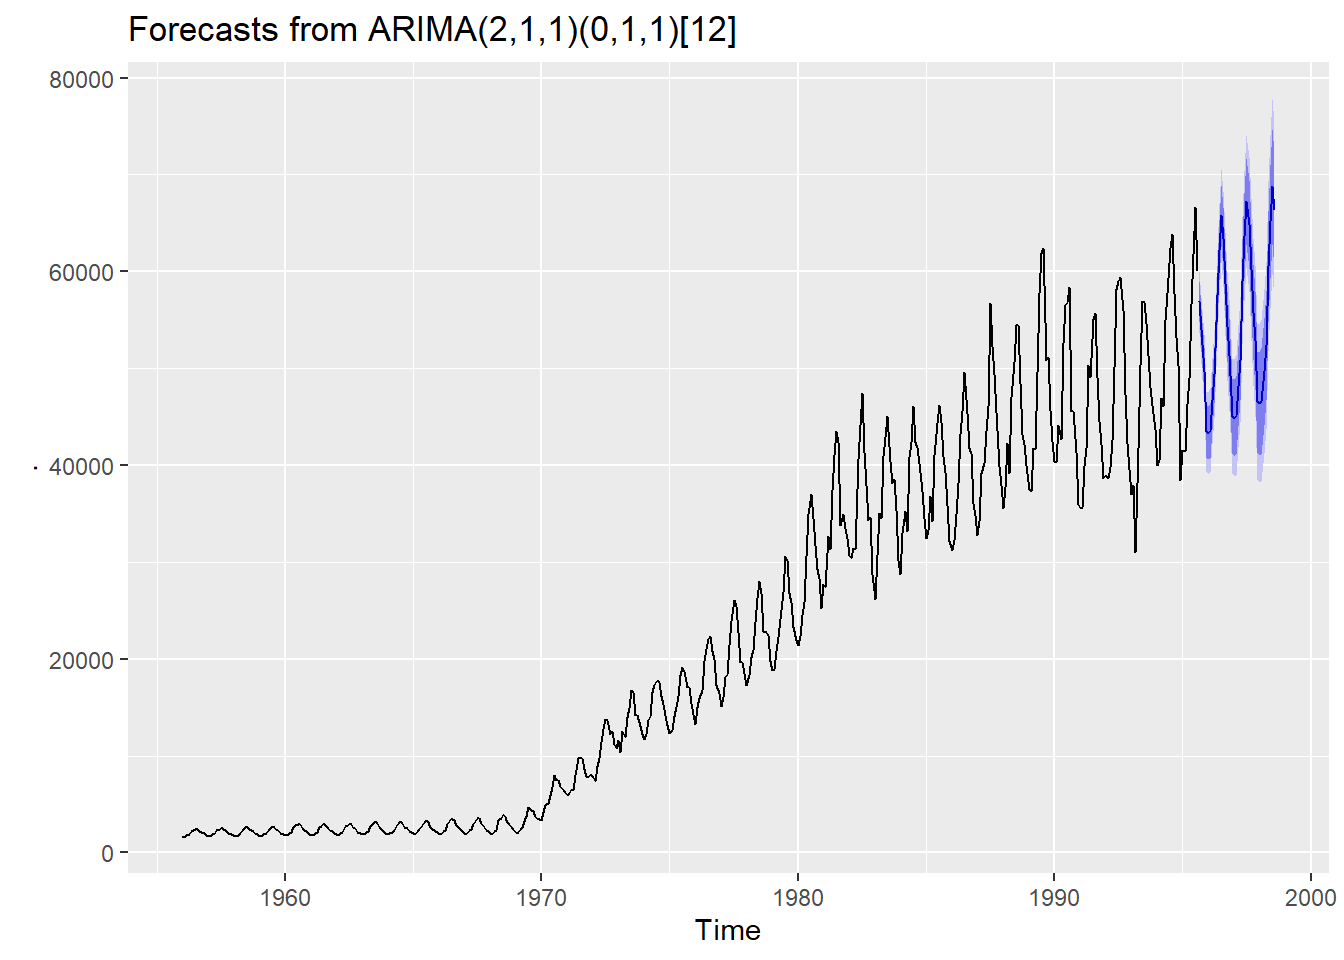
\includegraphics{RLearning_files/figure-latex/unnamed-chunk-44-1.pdf}

关于时间序列的分析与预测的更多信息可见\href{https://tidyverts.org/}{\passthrough{\lstinline!tidyverts!}系列包}, \href{https://pkg.robjhyndman.com/forecast/}{\passthrough{\lstinline!forecast!}包}等。

\hypertarget{ux591aux7ef4ux6570ux636eux7c7bux578b}{%
\subsection{多维数据类型}\label{ux591aux7ef4ux6570ux636eux7c7bux578b}}

之前我们讨论的数据类型都是一个序列(向量),都是一维的数据。在这章里我们会学习二维甚至多于二维的数据类型。

\hypertarget{ux77e9ux9635matrix}{%
\subsubsection{矩阵(matrix)}\label{ux77e9ux9635matrix}}

在R中的矩阵和数学概念上的矩阵很相似。在数学概念里,矩阵是一个按照长方阵列排列的数字集合,它有着固定的行数和列数。在R里,矩阵是一个按照长方阵列排列的、有着固定行数和列数的、包含同一类型数据的集合。你可以使用函数\passthrough{\lstinline!matrix!}来创建一个矩阵:

\begin{lstlisting}[language=R]
matrix(1:9, nrow = 3)
\end{lstlisting}

\begin{lstlisting}
##      [,1] [,2] [,3]
## [1,]    1    4    7
## [2,]    2    5    8
## [3,]    3    6    9
\end{lstlisting}

在这里,第一个参数是矩阵中数据的具体内容。\passthrough{\lstinline!1:9!} 是 \passthrough{\lstinline!c(1, 2, 3, 4, 5, 6, 7, 8, 9)!} 的一个缩写,用于创建间隔为1的整数序列。

第二个参数告诉R这个矩阵应该有多少行。你也可以使用\passthrough{\lstinline!ncol!}来告诉R这个矩阵有多少列。默认状态下,R会把数值按照从上到下、从左到右的顺序填充在这个固定行数列数的矩阵里。如果你想让R先从左到右填充(横向按照行填充),则需要将\passthrough{\lstinline!byrow!}参数设置为\passthrough{\lstinline!TRUE!}:

\begin{lstlisting}[language=R]
matrix(1:9, ncol = 3, byrow = TRUE)
\end{lstlisting}

\begin{lstlisting}
##      [,1] [,2] [,3]
## [1,]    1    2    3
## [2,]    4    5    6
## [3,]    7    8    9
\end{lstlisting}

R中的矩阵不局限于数值型矩阵,它只要求包含的数据从属于同一类型:如果是数值型,那每一个格子里都是数值型;如果是字符型,所有值都是字符型数据。

\begin{lstlisting}[language=R]
mat_month <- matrix(month.name, nrow = 4, byrow = TRUE)
mat_month
\end{lstlisting}

\begin{lstlisting}
##      [,1]      [,2]       [,3]       
## [1,] "January" "February" "March"    
## [2,] "April"   "May"      "June"     
## [3,] "July"    "August"   "September"
## [4,] "October" "November" "December"
\end{lstlisting}

\hypertarget{ux77e9ux9635ux547dux540d}{%
\paragraph{矩阵命名}\label{ux77e9ux9635ux547dux540d}}

对于一个矩阵来说,主要的命名集中于行名\passthrough{\lstinline!rownames!}和列名\passthrough{\lstinline!colnames!}:

\begin{lstlisting}[language=R]
# 你可以用这两个函数去更改行名和列名
rownames(mat_month) <- c("Quarter1", "Quarter2", "Quarter3", "Quarter4")
colnames(mat_month) <- c("Month1", "Month2", "Month3")

mat_month
\end{lstlisting}

\begin{lstlisting}
##          Month1    Month2     Month3     
## Quarter1 "January" "February" "March"    
## Quarter2 "April"   "May"      "June"     
## Quarter3 "July"    "August"   "September"
## Quarter4 "October" "November" "December"
\end{lstlisting}

\begin{lstlisting}[language=R]
# 也可以用这两个函数去获取行名和列名
rownames(mat_month)  
\end{lstlisting}

\begin{lstlisting}
## [1] "Quarter1" "Quarter2" "Quarter3" "Quarter4"
\end{lstlisting}

\begin{lstlisting}[language=R]
colnames(mat_month) 
\end{lstlisting}

\begin{lstlisting}
## [1] "Month1" "Month2" "Month3"
\end{lstlisting}

\begin{lstlisting}[language=R]
# 或者用一个函数获取所有维度的名称
dimnames(mat_month)
\end{lstlisting}

\begin{lstlisting}
## [[1]]
## [1] "Quarter1" "Quarter2" "Quarter3" "Quarter4"
## 
## [[2]]
## [1] "Month1" "Month2" "Month3"
\end{lstlisting}

\hypertarget{ux8bbfux95eeux77e9ux9635ux5b50ux96c6}{%
\paragraph{访问矩阵子集}\label{ux8bbfux95eeux77e9ux9635ux5b50ux96c6}}

和在向量里一样,访问矩阵的子集也可以用\passthrough{\lstinline![!}或者\passthrough{\lstinline![[!}。区别在于矩阵中我们有两个维度,所以需要同时给定两个维度的坐标:

\begin{lstlisting}[language=R]
# 访问矩阵中第1行第2列格子的元素
mat_month[[1, 2]]
\end{lstlisting}

\begin{lstlisting}
## [1] "February"
\end{lstlisting}

\begin{lstlisting}[language=R]
# 在逗号前不输入数字的时候
# 根据列号截取整列
mat_month[, 2]
\end{lstlisting}

\begin{lstlisting}
##   Quarter1   Quarter2   Quarter3   Quarter4 
## "February"      "May"   "August" "November"
\end{lstlisting}

\begin{lstlisting}[language=R]
# 在逗号后不输入数字的时候
# 根据行号截取整行
mat_month[1, ]
\end{lstlisting}

\begin{lstlisting}
##     Month1     Month2     Month3 
##  "January" "February"    "March"
\end{lstlisting}

\begin{lstlisting}[language=R]
# 如果有行名和列名的话
# 也可以用字符串来截取特定范围
mat_month[["Quarter1", "Month3"]]
\end{lstlisting}

\begin{lstlisting}
## [1] "March"
\end{lstlisting}

\hypertarget{ux5217ux8868list}{%
\subsubsection{列表(list)}\label{ux5217ux8868list}}

列表是R中比较基础的数据类型中最灵活的类型。它和向量或者矩阵不一样,在一个列表中可以储存各种不同的基本数据类型。你既可以存三个数字,也可以把数值型、字符型、逻辑型混合:

\begin{lstlisting}[language=R]
list(1, 2, 3)
\end{lstlisting}

\begin{lstlisting}
## [[1]]
## [1] 1
## 
## [[2]]
## [1] 2
## 
## [[3]]
## [1] 3
\end{lstlisting}

\begin{lstlisting}[language=R]
list(1, "lol", TRUE)
\end{lstlisting}

\begin{lstlisting}
## [[1]]
## [1] 1
## 
## [[2]]
## [1] "lol"
## 
## [[3]]
## [1] TRUE
\end{lstlisting}

列表甚至可以储存列表本身,也就意味着你可以一层套一层地设置列表。夹杂其他各种类型,就可以创造一个庞然大物:

\begin{lstlisting}[language=R]
stuff <- list(
  list(
    1:12, 
    "To be or not to be", 
    c(TRUE, FALSE)), 
  42, 
  list(
    list(
      ymd("2021-07-07"), 
      "remembrance"),
    2L+3i) 
)
stuff
\end{lstlisting}

\begin{lstlisting}
## [[1]]
## [[1]][[1]]
##  [1]  1  2  3  4  5  6  7  8  9 10 11 12
## 
## [[1]][[2]]
## [1] "To be or not to be"
## 
## [[1]][[3]]
## [1]  TRUE FALSE
## 
## 
## [[2]]
## [1] 42
## 
## [[3]]
## [[3]][[1]]
## [[3]][[1]][[1]]
## [1] "2021-07-07"
## 
## [[3]][[1]][[2]]
## [1] "remembrance"
## 
## 
## [[3]][[2]]
## [1] 2+3i
\end{lstlisting}

\hypertarget{ux8bbfux95eeux5b50ux5217ux8868}{%
\paragraph{访问子列表}\label{ux8bbfux95eeux5b50ux5217ux8868}}

列表同样可以用中括号来访问子列表。单个中括号\passthrough{\lstinline![!}和两个中括号\passthrough{\lstinline![[!}的区分在列表中特别重要。简单来说,单个中括号返回的列表元素类型还是列表,双中括号返回的列表元素是它本身的类型。想要返回多个子列表,就只能用单括号了,因为元素本身的类型不允许多个类型在一个序列中保存。

\begin{lstlisting}[language=R]
# 返回前两个子列表
stuff[1:2]
\end{lstlisting}

\begin{lstlisting}
## [[1]]
## [[1]][[1]]
##  [1]  1  2  3  4  5  6  7  8  9 10 11 12
## 
## [[1]][[2]]
## [1] "To be or not to be"
## 
## [[1]][[3]]
## [1]  TRUE FALSE
## 
## 
## [[2]]
## [1] 42
\end{lstlisting}

\begin{lstlisting}[language=R]
# 返回第一个子列表中的第二个子列表
stuff[[1]][[2]]
\end{lstlisting}

\begin{lstlisting}
## [1] "To be or not to be"
\end{lstlisting}

\hypertarget{ux5217ux8868ux547dux540d}{%
\paragraph{列表命名}\label{ux5217ux8868ux547dux540d}}

列表的维度,或者说层数可是比矩阵多多了,这也就意味着,列表中可以命名的地方多多了。

\begin{lstlisting}[language=R]
# 给列表的顶层三个列表命名
names(stuff) <- c("I", "II", "III")

# 给列表的第一个列表里的三个子列表命名
names(stuff[[1]]) <- c("I", "II", "III")
\end{lstlisting}

如果列表有名字,自然可以用包含名字的字符串获取子列表。

\begin{lstlisting}[language=R]
# 访问名为“I”的列表中名为“II”的子列表
stuff[["I"]][["II"]]
\end{lstlisting}

\begin{lstlisting}
## [1] "To be or not to be"
\end{lstlisting}

之前我们一直没有使用过美元符号\passthrough{\lstinline!$!}来获取子集,列表提供了一个最佳的展示场景,以下这行代码可以起到于上一行代码一样的效果,而不用加各种括号和引号:

\begin{lstlisting}[language=R]
stuff$I$II
\end{lstlisting}

\begin{lstlisting}
## [1] "To be or not to be"
\end{lstlisting}

\hypertarget{ux6570ux636eux8868data-frame-ux4e0e-tibble}{%
\subsubsection{数据表(data frame 与 tibble)}\label{ux6570ux636eux8868data-frame-ux4e0e-tibble}}

数据表将是进行数据分析的时候接触的最多的数据类型了。一个数据表(data frame)的本质是一个列表(list),但是采取了矩阵(matrix)的展示形式:

\begin{lstlisting}[language=R]
df <- data.frame(x = 1:12, y = month.abb, z = month.name)
df
\end{lstlisting}

\begin{lstlisting}
##     x   y         z
## 1   1 Jan   January
## 2   2 Feb  February
## 3   3 Mar     March
## 4   4 Apr     April
## 5   5 May       May
## 6   6 Jun      June
## 7   7 Jul      July
## 8   8 Aug    August
## 9   9 Sep September
## 10 10 Oct   October
## 11 11 Nov  November
## 12 12 Dec  December
\end{lstlisting}

数据表的每一列是一个子列表。将几个长度相同的子列表并排放在一起,就组成了一个长方形的矩阵形式。这种特殊的处理使得数据表包含了两种数据形式的优势。列与列之间可以使用不同的基础数据类型,也就是说一列的数据是数值型的数据,下一列数据可以是字符型的数据。长方形的形状保证了列与列之间的数值是一一对应的,每一行都是一个观察量。这很符合日常会遇到的数据的形式。

\passthrough{\lstinline!tibble!}是\passthrough{\lstinline!tidyverse!}系列包中的\passthrough{\lstinline!tibble!}包提供的一种数据形式。使用\passthrough{\lstinline!tibble!}比较明显的好处是,当你把\passthrough{\lstinline!tibble!}打印在控制台里的时候,它有一个更干净直观的打印方式。与 data frame 试图打印所有的行、一股脑把所有信息扔给你不同,\passthrough{\lstinline!tibble!} 默认只会打印前几行给你一个数据长什么样的感觉,还会告诉你每一列的数据是什么类型的:

\begin{lstlisting}[language=R]
tb <- tibble(a = 1:100, b = 101:200)
tb
\end{lstlisting}

\begin{lstlisting}
## # A tibble: 100 x 2
##        a     b
##    <int> <int>
##  1     1   101
##  2     2   102
##  3     3   103
##  4     4   104
##  5     5   105
##  6     6   106
##  7     7   107
##  8     8   108
##  9     9   109
## 10    10   110
## # ... with 90 more rows
\end{lstlisting}

除了看起来好看以外,\passthrough{\lstinline!tibble!}在原始数据表的基础上保留了有用的功能,去除了多余的功能。它干得更少,比如它不会自发修改变量类型或变量名字,也不会做部分匹配;同时它抱怨得更多,比如当一个变量不存在的时候就会触发错误信息。这样用户就能及早发现错误,不会等到代码堆成小💩山。

\hypertarget{ux8bbfux95eeux6570ux636eux8868ux5185ux5bb9}{%
\paragraph{访问数据表内容}\label{ux8bbfux95eeux6570ux636eux8868ux5185ux5bb9}}

既然看上去像矩阵,听起来像列表,那就应该可以用适用于矩阵和列表的方法访问数据表元素。事实上也的确是这样:

\begin{lstlisting}[language=R]
# 访问数据表名为x的列
df[["x"]]
\end{lstlisting}

\begin{lstlisting}
##  [1]  1  2  3  4  5  6  7  8  9 10 11 12
\end{lstlisting}

\begin{lstlisting}[language=R]
df$x
\end{lstlisting}

\begin{lstlisting}
##  [1]  1  2  3  4  5  6  7  8  9 10 11 12
\end{lstlisting}

\begin{lstlisting}[language=R]
# 访问第一行第二个数值
df[1, 2]
\end{lstlisting}

\begin{lstlisting}
## [1] "Jan"
\end{lstlisting}

\begin{lstlisting}[language=R]
# 访问tibble第2列
tb[, 2]
\end{lstlisting}

\begin{lstlisting}
## # A tibble: 100 x 1
##        b
##    <int>
##  1   101
##  2   102
##  3   103
##  4   104
##  5   105
##  6   106
##  7   107
##  8   108
##  9   109
## 10   110
## # ... with 90 more rows
\end{lstlisting}

\begin{lstlisting}[language=R]
# 访问tibble第1行第2列的数值
tb[1, 2]
\end{lstlisting}

\begin{lstlisting}
## # A tibble: 1 x 1
##       b
##   <int>
## 1   101
\end{lstlisting}

\begin{lstlisting}[language=R]
tb$a
#太长了还是不显示了吧
\end{lstlisting}

tibble 的另一个特性是其访问的子列表也是\passthrough{\lstinline!tibble!}类型的数据表,即使是用单引号返回一个格子的元素。

关于\passthrough{\lstinline!tibble!}更多信息,详见\href{https://tibble.tidyverse.org/}{\passthrough{\lstinline!tibble!}主页}。

\hypertarget{ux8bfbux5199ux6570ux636e}{%
\subsection{读写数据}\label{ux8bfbux5199ux6570ux636e}}

这一章我们主要讨论根据不同数据保存方式区分的读写数据的方法。

\hypertarget{ux5185ux7f6eux6570ux636eux96c6}{%
\subsubsection{内置数据集}\label{ux5185ux7f6eux6570ux636eux96c6}}

R本身和一些R包都会有内置的数据集。使用\passthrough{\lstinline!data!}命令来查看、使用可用数据集。

\begin{lstlisting}[language=R]
# 查看R本身自带的数据集
data()

# 查看某一R包自带的数据集
data(package = "dplyr")
\end{lstlisting}

\begin{lstlisting}[language=R]
# 载入AirPassengers数据集
data("AirPassengers")

glimpse(AirPassengers)
\end{lstlisting}

\begin{lstlisting}
##  Time-Series [1:144] from 1949 to 1961: 112 118 132 129 121 135 148 148 136 119 ...
\end{lstlisting}

\hypertarget{ux8868ux683cux7c7bux578bux6570ux636ecsv-excel}{%
\subsubsection{表格类型数据(csv, excel)}\label{ux8868ux683cux7c7bux578bux6570ux636ecsv-excel}}

h1n1 流感问卷数据储存在名为 ``h1n1\_flu.csv'' 的文件中,我们会在下一篇《数据清洗与准备》中用到。假设 ``h1n1\_flu'' 有不同的储存类型,我们列举一些读写数据表类型数据的方法。

\begin{lstlisting}[language=R]
# 读取csv文件
library(readr)
h1n1_flu <- read_csv("h1n1_flu.csv")
# 保存csv文件
write_csv(h1n1_flu, "h1n1_flu.csv")


# 读取excel文件
library(readxl)
# 自动识别文件后缀
h1n1_flu <- read_excel("h1n1_flu.xls")
# 读取xls文件
h1n1_flu <- read_xls("h1n1_flu.xls")
# 读取xlsx文件
h1n1_flu <- read_xlsx("h1n1_flu.xlsx")
\end{lstlisting}

不建议在R中直接编辑 excel 文件,csv 文件应该满足日常所需了。如果有编辑 excel 文件的需求,可以看看\passthrough{\lstinline!openxlsx!}包。

\hypertarget{rux7684ux4e13ux5c5eux7c7bux578bux6570ux636erdata-rds}{%
\subsubsection{R的专属类型数据(RData, rds)}\label{rux7684ux4e13ux5c5eux7c7bux578bux6570ux636erdata-rds}}

有一些数据存储方式是R中独有的。我们在这里讨论两类。一类是 rds 文件,一类是 RData 文件。

\begin{enumerate}
\def\labelenumi{\arabic{enumi}.}
\tightlist
\item
  rds 文件储存一个R中的对象。这个对象不一定是四四方方的数据表,而可以是任何形式,包括复杂的列表等。因为他储存的是一个对象,所以读取的时候也是读取出来一个对象,需要被保存在一个名字下。
\item
  RData 储存的是一个或多个、任意结构的、带有自己名字的对象。读取的时候会将储存的对象直接载入当前的环境中,使用的是对象自己的名字,所以不需要再额外起名字。
\end{enumerate}

\begin{lstlisting}[language=R]
# 读取
h1n1_flu <- read_rds("h1n1_flu.rds")
# 存储
write_rds(h1n1_flu, "h1n1_flu.rds")

# 读取
load("h1n1_flu.RData")
# 存储
save(h1n1_flu, file = "h1n1_flu.RData")
\end{lstlisting}

\hypertarget{ux5176ux4ed6ux8f6fux4ef6spss-stata-sas}{%
\subsubsection{其他软件(SPSS, Stata, SAS)}\label{ux5176ux4ed6ux8f6fux4ef6spss-stata-sas}}

R也可以直接读取其他软件的数据类型。这里列举使用\passthrough{\lstinline!haven!}包读写 SPSS 的 sav 和 zsav、 Stata 的 dta、SAS 的 sas7bdat 和 sas7bcat。

\begin{lstlisting}[language=R]
library(haven)

# SPSS
read_spss()
write_spss()

# Stata
read_dta() 
write_dta() 

# SAS
read_sas()
write_sas()
\end{lstlisting}

\hypertarget{ux7ec3ux4e60ux9898}{%
\subsection{练习题}\label{ux7ec3ux4e60ux9898}}

\hypertarget{ux4e86ux89e3ux6570ux636eux96c6}{%
\subsubsection{了解数据集}\label{ux4e86ux89e3ux6570ux636eux96c6}}

请使用之前读取的\passthrough{\lstinline!h1n1\_flu!}完成以下任务。

\hypertarget{ux5e38ux7528ux6570ux636eux63a2ux67e5ux51fdux6570}{%
\paragraph{常用数据探查函数}\label{ux5e38ux7528ux6570ux636eux63a2ux67e5ux51fdux6570}}

请尝试使用以下常用的数据探查函数,挑出两个你最喜欢的描述他们的功能。别忘了可以用\passthrough{\lstinline!?fun!}查看帮助文档。

\begin{lstlisting}[language=R]
glimpse(h1n1_flu)
str(h1n1_flu)
head(h1n1_flu)
tail(h1n1_flu)
View(h1n1_flu)
summary(h1n1_flu)
nrow(h1n1_flu)
length(h1n1_flu$sex)
class(h1n1_flu$sex)
summary(h1n1_flu)
table(h1n1_flu$sex)
\end{lstlisting}

\hypertarget{ux5206ux7ec4ux8ba1ux7b97ux7edfux8ba1ux91cf}{%
\paragraph{分组计算统计量}\label{ux5206ux7ec4ux8ba1ux7b97ux7edfux8ba1ux91cf}}

\begin{lstlisting}[language=R]
h1n1_flu %>% 
  group_by(sex, employment_status) %>% 
  summarise(n())
\end{lstlisting}

\begin{lstlisting}
## # A tibble: 8 x 3
## # Groups:   sex [2]
##   sex    employment_status  `n()`
##   <chr>  <chr>              <int>
## 1 Female Employed            7416
## 2 Female Not in Labor Force  6918
## 3 Female Unemployed           735
## 4 Female <NA>                 789
## 5 Male   Employed            6144
## 6 Male   Not in Labor Force  3313
## 7 Male   Unemployed           718
## 8 Male   <NA>                 674
\end{lstlisting}

请问上边这几行代码在计算什么?你可不可以使用同样的方法计算一些其他的统计量?别忘了看看帮助文档\passthrough{\lstinline!?summarise!}。

\hypertarget{ux521bux9020ux6570ux636eux96c6}{%
\subsubsection{创造数据集}\label{ux521bux9020ux6570ux636eux96c6}}

我们说过数据表的本质是将列表排列在一起,所以数据表就会有列表的性质。而我们又知道列表可以包含任何类型的数据,无论是单个的数值或者是向量、矩阵等。

\begin{enumerate}
\def\labelenumi{\arabic{enumi}.}
\tightlist
\item
  请你创造一个数据表,其中的某一列变量的每一个格子包含的不再是常规的单个数值或者字符串,而是一个向量或者矩阵等多维的数据类型;
\item
  请你描述一个可以在数据分析时运用此类特性的使用场景。
\end{enumerate}

\hypertarget{ux672cux7ae0ux4f5cux8005-1}{%
\subsection*{本章作者}\label{ux672cux7ae0ux4f5cux8005-1}}


\textbf{Fin}

\begin{quote}
\url{https://yangzhuoranyang.com}
\end{quote}

\hypertarget{ux5173ux4e8edatawhale-1}{%
\subsection*{关于Datawhale}\label{ux5173ux4e8edatawhale-1}}


Datawhale 是一个专注于数据科学与AI领域的开源组织,汇集了众多领域院校和知名企业的优秀学习者,聚合了一群有开源精神和探索精神的团队成员。Datawhale 以``for the learner,和学习者一起成长''为愿景,鼓励真实地展现自我、开放包容、互信互助、敢于试错和勇于担当。同时 Datawhale 用开源的理念去探索开源内容、开源学习和开源方案,赋能人才培养,助力人才成长,建立起人与人,人与知识,人与企业和人与未来的联结。 本次数据挖掘路径学习,专题知识将在天池分享,详情可关注 Datawhale:


\includegraphics[width=3.58in]{image/logo}

\hypertarget{task-02}{%
\section{数据清洗与准备}\label{task-02}}

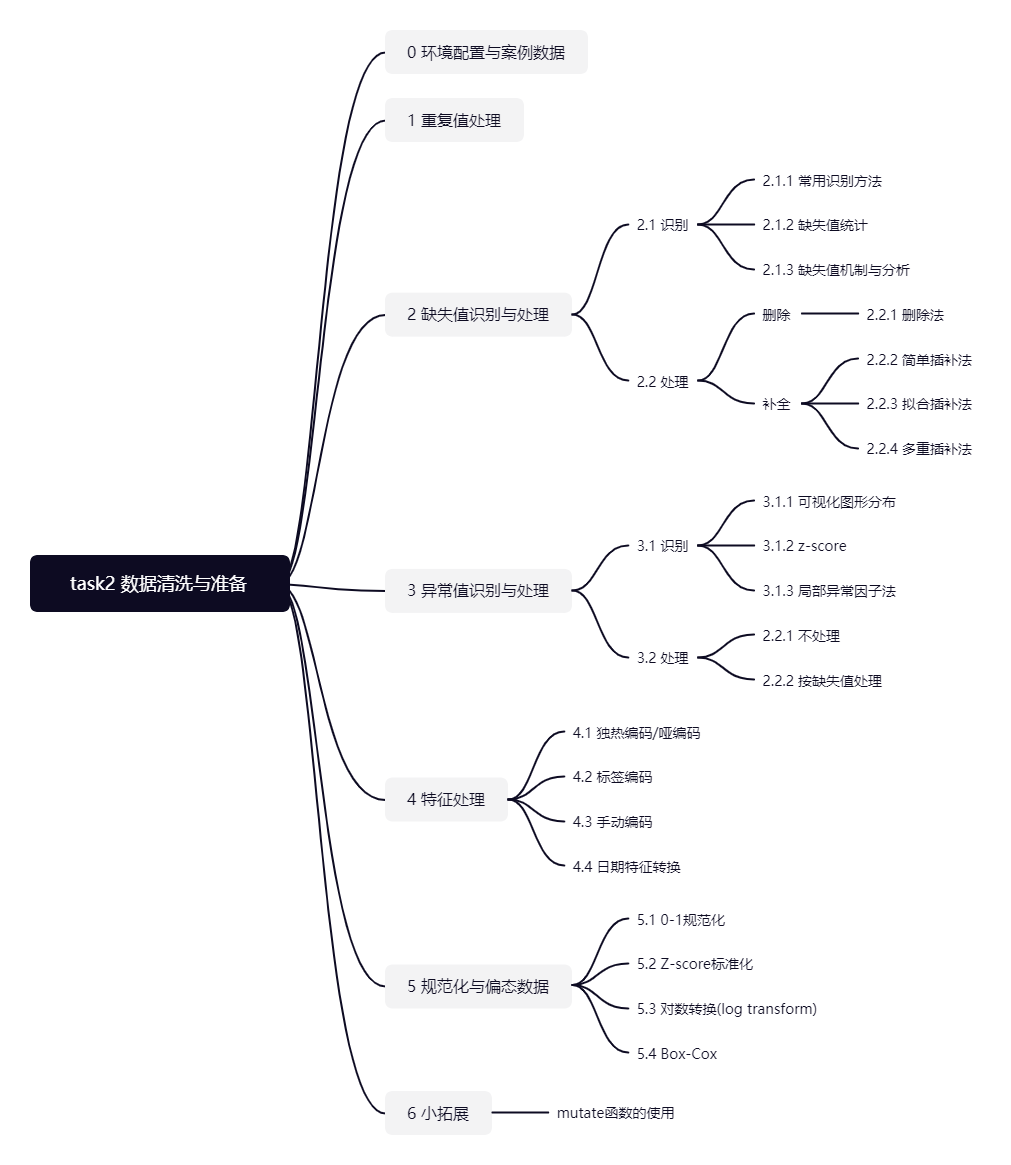
\includegraphics[width=1\textwidth,height=\textheight]{./image/task02_structure.jpg}

Task 02共计6个知识点,预计需学习5\textasciitilde8小时,请安排好学习任务。

\hypertarget{ux73afux5883ux914dux7f6e-1}{%
\subsection*{环境配置}\label{ux73afux5883ux914dux7f6e-1}}


\begin{lstlisting}[language=R]
library(mlbench) # 将会使用到包中的BostonHousing数据集
library(funModeling) # 探索性数据分析工具包,本节内容中将会使用到它的status()函数,打印整体数据质量
library(tidyverse) # 数据转化工具包,本节内容中将会使用它包含的dplyr中的管道函数 %>%
library(VIM) # 缺失值可视化工具包,本节内容中将会使用到它的aggr()函数
library(mice) # 缺失值处理工具包,本节内容会使用它来进行多重插补
library(Rlof) # 用于LOF异常值检测方法,本节内容将会使用到它的lof()函数
library(fastDummies) # 用于生成dummy的包,本节内容将会使用到它的dummy_cols()函数
library(sjmisc) # 用于生成dummy的包,本节内容将会使用到它的to_dummy()函数
library(MASS) # 基于此包进行box-cox转换
library(dlookr) # 本节内容将会使用到它的transform()函数
\end{lstlisting}

\hypertarget{ux6848ux4f8bux6570ux636e}{%
\subsection*{案例数据}\label{ux6848ux4f8bux6570ux636e}}


本节内容将会使用到两个数据集。

\hypertarget{ux6570ux636eux96c61-h1n1ux6d41ux611fux95eeux5377ux6570ux636eux96c6}{%
\subsubsection*{数据集1 h1n1流感问卷数据集}\label{ux6570ux636eux96c61-h1n1ux6d41ux611fux95eeux5377ux6570ux636eux96c6}}


\hypertarget{ux6570ux636eux8bf4ux660e}{%
\paragraph*{数据说明}\label{ux6570ux636eux8bf4ux660e}}
\addcontentsline{toc}{paragraph}{数据说明}

目前提供的数据集来自关于h1n1流感调查问卷的部分内容,可以从这个网站上看到具体字段的详细说明:\url{https://www.drivendata.org/competitions/66/flu-shot-learning/page/211/}

数据集包含26,707个受访者数据,共有32个特征+1个标签(是否接种h1n1疫苗)。

\hypertarget{ux52a0ux8f7dux5e76ux67e5ux770bux90e8ux5206ux6570ux636e}{%
\paragraph*{加载并查看部分数据}\label{ux52a0ux8f7dux5e76ux67e5ux770bux90e8ux5206ux6570ux636e}}
\addcontentsline{toc}{paragraph}{加载并查看部分数据}

首先加载数据,了解数据集大小。

\begin{lstlisting}[language=R]
h1n1_data <- read.csv("./datasets/h1n1_flu.csv", header = TRUE)
dim(h1n1_data)
\end{lstlisting}

\begin{lstlisting}
## [1] 26707    33
\end{lstlisting}

注:为了简化本章的示例,我们在这32个特征中,筛选出了10个特征,作为一个子集,来学习如何使用R做数据清洗与准备。如有兴趣,可以把下面这块筛选去掉,自己用完整数据集做一次探索。

\begin{lstlisting}[language=R]
h1n1_data <- h1n1_data[, c(1, 3, 11, 12, 15, 16, 19, 20, 22, 23, 33)]
head(h1n1_data)
\end{lstlisting}

\begin{lstlisting}
##   respondent_id h1n1_knowledge doctor_recc_h1n1 chronic_med_condition
## 1             0              0                0                     0
## 2             1              2                0                     0
## 3             2              1               NA                     1
## 4             3              1                0                     1
## 5             4              1                0                     0
## 6             5              1                0                     0
##   health_insurance opinion_h1n1_vacc_effective     age_group        education
## 1                1                           3 55 - 64 Years       < 12 Years
## 2                1                           5 35 - 44 Years         12 Years
## 3               NA                           3 18 - 34 Years College Graduate
## 4               NA                           3     65+ Years         12 Years
## 5               NA                           3 45 - 54 Years     Some College
## 6               NA                           5     65+ Years         12 Years
##      sex            income_poverty h1n1_vaccine
## 1 Female             Below Poverty            0
## 2   Male             Below Poverty            0
## 3   Male <= $75,000, Above Poverty            0
## 4 Female             Below Poverty            0
## 5 Female <= $75,000, Above Poverty            0
## 6   Male <= $75,000, Above Poverty            0
\end{lstlisting}

\hypertarget{ux6570ux636eux96c62-ux6ce2ux58ebux987fux623fux4ef7ux6570ux636eux96c6}{%
\subsubsection*{数据集2 波士顿房价数据集}\label{ux6570ux636eux96c62-ux6ce2ux58ebux987fux623fux4ef7ux6570ux636eux96c6}}


\hypertarget{ux6570ux636eux8bf4ux660e-1}{%
\paragraph*{数据说明}\label{ux6570ux636eux8bf4ux660e-1}}
\addcontentsline{toc}{paragraph}{数据说明}

数据集来自\passthrough{\lstinline!mlbench!}包,请提前装好。数据字段说明可从网址查看:\url{https://blog.csdn.net/weixin_46027193/article/details/112238597}

数据集包含506条房价信息,共有13个特征+1个预测字段(房屋价格)。

\hypertarget{ux52a0ux8f7dux5e76ux67e5ux770bux90e8ux5206ux6570ux636e-1}{%
\paragraph*{加载并查看部分数据}\label{ux52a0ux8f7dux5e76ux67e5ux770bux90e8ux5206ux6570ux636e-1}}
\addcontentsline{toc}{paragraph}{加载并查看部分数据}

\begin{lstlisting}[language=R]
data(BostonHousing)
dim(BostonHousing)
\end{lstlisting}

\begin{lstlisting}
## [1] 506  14
\end{lstlisting}

\begin{lstlisting}[language=R]
head(BostonHousing)
\end{lstlisting}

\begin{lstlisting}
##      crim zn indus chas   nox    rm  age    dis rad tax ptratio      b lstat
## 1 0.00632 18  2.31    0 0.538 6.575 65.2 4.0900   1 296    15.3 396.90  4.98
## 2 0.02731  0  7.07    0 0.469 6.421 78.9 4.9671   2 242    17.8 396.90  9.14
## 3 0.02729  0  7.07    0 0.469 7.185 61.1 4.9671   2 242    17.8 392.83  4.03
## 4 0.03237  0  2.18    0 0.458 6.998 45.8 6.0622   3 222    18.7 394.63  2.94
## 5 0.06905  0  2.18    0 0.458 7.147 54.2 6.0622   3 222    18.7 396.90  5.33
## 6 0.02985  0  2.18    0 0.458 6.430 58.7 6.0622   3 222    18.7 394.12  5.21
##   medv
## 1 24.0
## 2 21.6
## 3 34.7
## 4 33.4
## 5 36.2
## 6 28.7
\end{lstlisting}

\hypertarget{ux91cdux590dux503cux5904ux7406}{%
\subsection{重复值处理}\label{ux91cdux590dux503cux5904ux7406}}

在某些情况下,我们需要对数据进行去重处理。\passthrough{\lstinline!unique()!}函数可以对数据进行整体去重,\passthrough{\lstinline!distinct()!}函数可以针对某些列去重。

\begin{lstlisting}[language=R]
# 整体去重
h1n1_data_de_dup1 <- unique(h1n1_data)

# 指定根据列respondent_id,h1n1_knowledge去重,并保留所有列
h1n1_data_de_dup2 <- distinct(h1n1_data, respondent_id, h1n1_knowledge, .keep_all = T)
\end{lstlisting}

\hypertarget{ux7f3aux5931ux503cux8bc6ux522bux4e0eux5904ux7406}{%
\subsection{缺失值识别与处理}\label{ux7f3aux5931ux503cux8bc6ux522bux4e0eux5904ux7406}}

现实环境中,由于数据来源及搜集过程,可能有各种不规范,导致数据往往会存在缺失。缺失值识别与处理,无论是在统计还是数据管理中,往往是数据清洗的第一步。

\hypertarget{ux7f3aux5931ux503cux8bc6ux522b}{%
\subsubsection{缺失值识别}\label{ux7f3aux5931ux503cux8bc6ux522b}}

\hypertarget{ux5e38ux7528ux8bc6ux522bux65b9ux6cd5}{%
\paragraph{常用识别方法}\label{ux5e38ux7528ux8bc6ux522bux65b9ux6cd5}}

在R语言中,惯用会把缺失值表示为NA,一般可使用\passthrough{\lstinline!is.na(a)!},\passthrough{\lstinline"!complete.cases(a)"}来识别\passthrough{\lstinline!a!}是否为缺失值。

\begin{lstlisting}[language=R]
# 假设定义的一个变量中存在缺失值
y <- c(1, 2, 3, NA)

# 用is.na在识别是否为缺失值
is.na(y)
\end{lstlisting}

\begin{lstlisting}
## [1] FALSE FALSE FALSE  TRUE
\end{lstlisting}

\begin{lstlisting}[language=R]
# 用!complete.cases()在识别是否为缺失值
!complete.cases(y)
\end{lstlisting}

\begin{lstlisting}
## [1] FALSE FALSE FALSE  TRUE
\end{lstlisting}

\hypertarget{ux7f3aux5931ux503cux7edfux8ba1}{%
\paragraph{缺失值统计}\label{ux7f3aux5931ux503cux7edfux8ba1}}

统计缺失值总数。

\begin{lstlisting}[language=R]
# 数据集中总缺失数据量
sum(is.na(h1n1_data))
\end{lstlisting}

\begin{lstlisting}
## [1] 15912
\end{lstlisting}

\begin{lstlisting}[language=R]
# 数据集中某一列缺失数据量
sum(is.na(h1n1_data["h1n1_knowledge"]))
\end{lstlisting}

\begin{lstlisting}
## [1] 116
\end{lstlisting}

如果想按行或按列统计,可以写函数。

\begin{lstlisting}[language=R]
pMiss <- function(x) {
  sum(is.na(x)) / length(x) * 100
}
apply(h1n1_data, 2, pMiss) # 按列统计缺失比率%
\end{lstlisting}

\begin{lstlisting}
##               respondent_id              h1n1_knowledge 
##                   0.0000000                   0.4343431 
##            doctor_recc_h1n1       chronic_med_condition 
##                   8.0877673                   3.6357509 
##            health_insurance opinion_h1n1_vacc_effective 
##                  45.9579885                   1.4640356 
##                   age_group                   education 
##                   0.0000000                   0.0000000 
##                         sex              income_poverty 
##                   0.0000000                   0.0000000 
##                h1n1_vaccine 
##                   0.0000000
\end{lstlisting}

\begin{lstlisting}[language=R]
# apply(h1n1_data,1,pMiss) #按行统计缺失比率%
\end{lstlisting}

或调用一些现成的包。比如,我们可以使用\passthrough{\lstinline!funModeling!}包中的\passthrough{\lstinline!status()!}函数,直接观测案例数据中包含的0值,缺失值(NA),在每个特征中的分布情况。以h1n1 flu数据集为例:

\begin{lstlisting}[language=R]
data_quality <- status(h1n1_data)
data_quality %>% mutate(across(where(is.numeric), ~ round(., 3))) # 保留4位小数
\end{lstlisting}

\begin{lstlisting}
##                                                variable q_zeros p_zeros  q_na
## respondent_id                             respondent_id       1   0.000     0
## h1n1_knowledge                           h1n1_knowledge    2506   0.094   116
## doctor_recc_h1n1                       doctor_recc_h1n1   19139   0.717  2160
## chronic_med_condition             chronic_med_condition   18446   0.691   971
## health_insurance                       health_insurance    1736   0.065 12274
## opinion_h1n1_vacc_effective opinion_h1n1_vacc_effective       0   0.000   391
## age_group                                     age_group       0   0.000     0
## education                                     education       0   0.000     0
## sex                                                 sex       0   0.000     0
## income_poverty                           income_poverty       0   0.000     0
## h1n1_vaccine                               h1n1_vaccine   21033   0.788     0
##                              p_na q_inf p_inf      type unique
## respondent_id               0.000     0     0   integer  26707
## h1n1_knowledge              0.004     0     0   numeric      3
## doctor_recc_h1n1            0.081     0     0   numeric      2
## chronic_med_condition       0.036     0     0   numeric      2
## health_insurance            0.460     0     0   numeric      2
## opinion_h1n1_vacc_effective 0.015     0     0   numeric      5
## age_group                   0.000     0     0 character      5
## education                   0.000     0     0 character      5
## sex                         0.000     0     0 character      2
## income_poverty              0.000     0     0 character      4
## h1n1_vaccine                0.000     0     0   integer      2
\end{lstlisting}

结合案例数据h1n1 flu来看,存在缺失值的有5个特征字段。

\begin{lstlisting}[language=R]
missing_Value <- data_quality[which(data_quality$p_na > 0), ]
missing_Value$variable
\end{lstlisting}

\begin{lstlisting}
## [1] "h1n1_knowledge"              "doctor_recc_h1n1"           
## [3] "chronic_med_condition"       "health_insurance"           
## [5] "opinion_h1n1_vacc_effective"
\end{lstlisting}

\hypertarget{ux7f3aux5931ux503cux673aux5236ux4e0eux5206ux6790}{%
\paragraph{缺失值机制与分析}\label{ux7f3aux5931ux503cux673aux5236ux4e0eux5206ux6790}}

统计学家通常将缺失数据分为3类,为了更好的处理缺失值,我们可以基于缺失值机制来识别以下3种缺失模式:

\begin{itemize}
\tightlist
\item
  MCAR(完全随机缺失):如果数据的缺失与任何值(观察或缺失)之间没有关系,则为MCAR。
\item
  MAR(随机缺失):考虑MAR与MCAR有何不同,如果缺失和观测值之间存在系统关系,则为MAR。例如-男性比女性更容易告诉自己的体重,因此体重就是MAR。`` Weight''变量的缺失取决于变量``Sex''的观测值。
\item
  MNAR(非随机缺失):若缺失数据不属于MCAR和MAR,数据的缺失依赖于不完全变量本身,则数据为非随机缺失。例如,抑郁程度高的人更不容易填写抑郁调查问卷。
\end{itemize}

MNAR是最复杂的情况,处理 MNAR的策略是找到更多有关缺失原因的数据,或者执行假设分析,查看结果在各种情况下的敏感程度。大部分处理缺失数据的方法都假定数据是MCAR或MAR,此时,可以忽略缺失数据的生成机制,在替换或删除缺失数据后,直接对感兴趣的关系进行建模。

以下介绍几种可视化分析缺失数据关联的方法:

我们用\passthrough{\lstinline!VIM!}包里的\passthrough{\lstinline!aggr()!}函数,直观看一下具体的缺失情况。

\begin{lstlisting}[language=R]
aggr(h1n1_data, cex.axis = .6, oma = c(9, 5, 5, 1)) # cex.axis调整轴字体大小,oma调整外边框大小
\end{lstlisting}

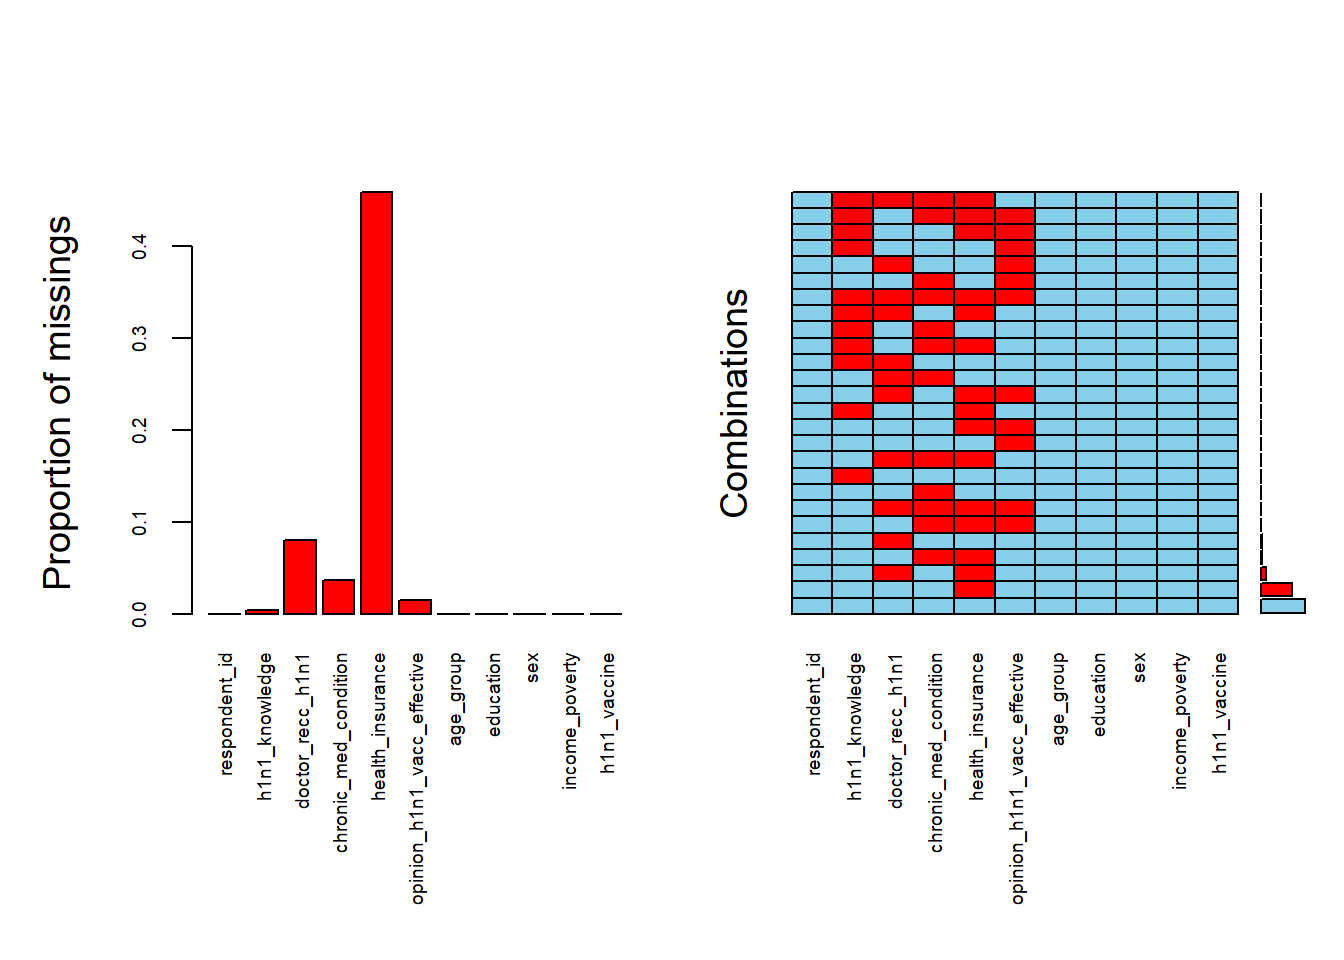
\includegraphics{RLearning_files/figure-latex/unnamed-chunk-80-1.pdf}

通过用\passthrough{\lstinline!VIM!}包里的矩阵图\passthrough{\lstinline!matrixplot()!}函数,可以检查某些变量的缺失值模式是否与其他变量的真实值有关联。矩阵图中,观测数据以黑白色阶显示(颜色越深,数值越高),缺失值会被标记为红色。我们对某一个存在缺失值的变量进行排序,来找寻含缺失值变量与其他变量的关系。

在此案例中,我们按照\passthrough{\lstinline!health\_insurance!}进行分组排序。可以看到是否有慢性病\passthrough{\lstinline!chronic\_med\_condition!}的缺失,与\passthrough{\lstinline!opinion\_h1n1\_vacc\_effective!}的缺失相对较集中。除此之外,也可以看到有慢性病的人年龄普遍较大。

\begin{lstlisting}[language=R]
# 先简单处理一下一些类别变量的顺序
h1n1_data_matplt <- h1n1_data
h1n1_data_matplt$age_group <- factor(h1n1_data_matplt$age_group)
h1n1_data_matplt$education <- factor(h1n1_data_matplt$education, levels = c("", "< 12 Years", "12 Years", "Some College", "College Graduate"))
h1n1_data_matplt$sex <- factor(h1n1_data_matplt$sex)
h1n1_data_matplt$income_poverty <- factor(h1n1_data_matplt$income_poverty, levels = c("18 - 34 Years", "<= $75,000, Above Poverty", "> $75,000"))
# levels(h1n1_data_matplt$age_group) # 查看顺序

# 矩阵图可视化
par(mar = c(9, 4.1, 2.1, 2.1)) # x轴标签太长,调用par()函数调整外边框的大小
matrixplot(h1n1_data_matplt, sortby = "chronic_med_condition", cex.axis = 0.7) # cex.axis为调整坐标轴字体大小
\end{lstlisting}

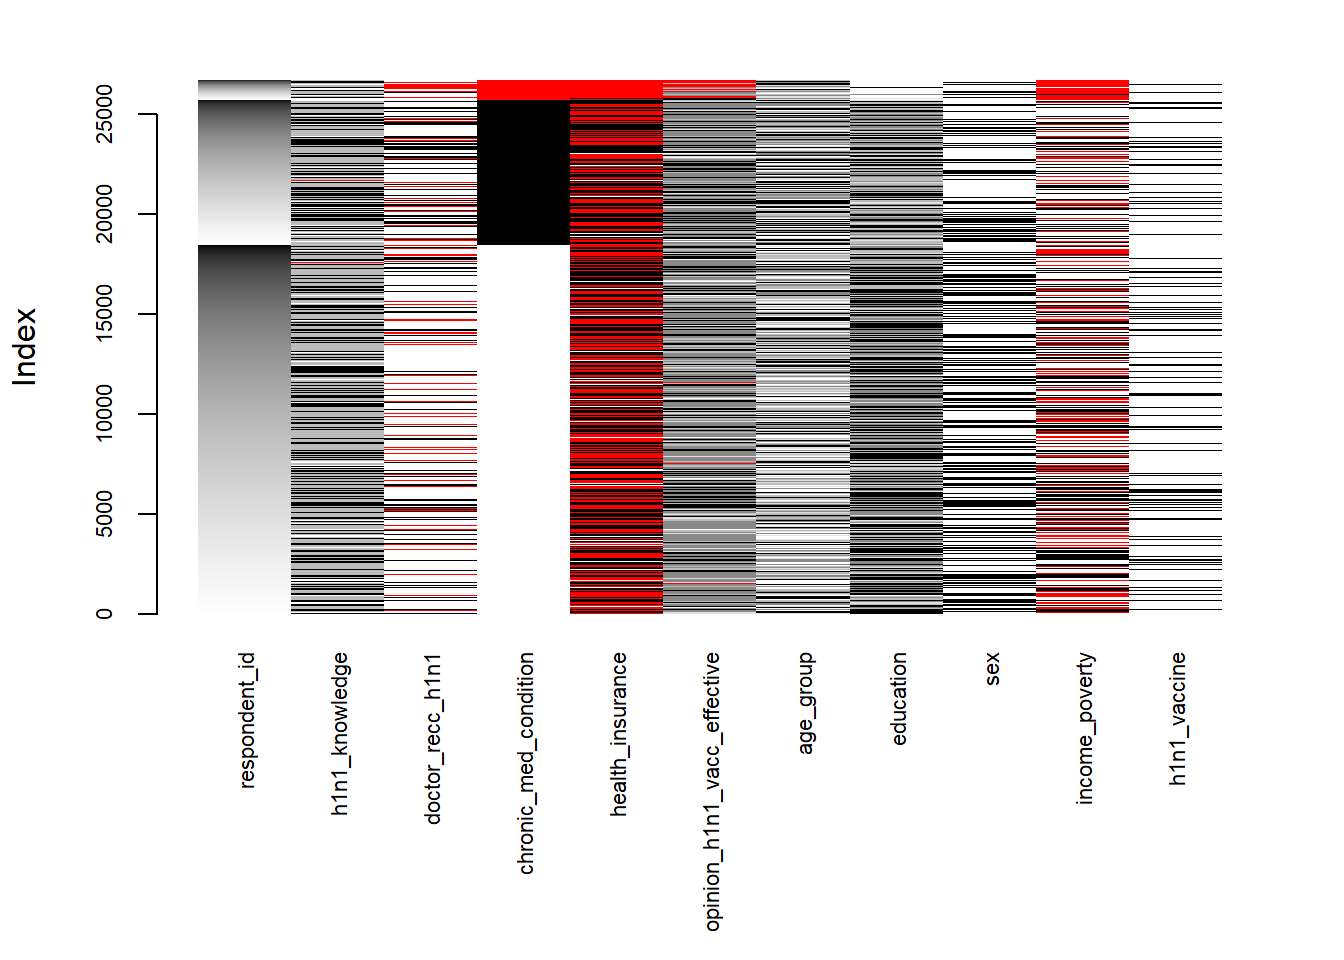
\includegraphics{RLearning_files/figure-latex/unnamed-chunk-81-1.pdf}

用相关性探索缺失值。首先生成一个影子矩阵,用指示变量替代数据集中的数据(1表示缺失,0表示存在)。

\begin{lstlisting}[language=R]
shadow_mat <- as.data.frame(abs(is.na(h1n1_data[, -1])))
head(shadow_mat)
\end{lstlisting}

\begin{lstlisting}
##   h1n1_knowledge doctor_recc_h1n1 chronic_med_condition health_insurance
## 1              0                0                     0                0
## 2              0                0                     0                0
## 3              0                1                     0                1
## 4              0                0                     0                1
## 5              0                0                     0                1
## 6              0                0                     0                1
##   opinion_h1n1_vacc_effective age_group education sex income_poverty
## 1                           0         0         0   0              0
## 2                           0         0         0   0              0
## 3                           0         0         0   0              0
## 4                           0         0         0   0              0
## 5                           0         0         0   0              0
## 6                           0         0         0   0              0
##   h1n1_vaccine
## 1            0
## 2            0
## 3            0
## 4            0
## 5            0
## 6            0
\end{lstlisting}

\begin{lstlisting}[language=R]
# 可提取含缺失值的变量
shadow_mat <- shadow_mat[which(apply(shadow_mat, 2, sum) > 0)]

# 计算相关系数
cor(shadow_mat)
\end{lstlisting}

\begin{lstlisting}
##                             h1n1_knowledge doctor_recc_h1n1
## h1n1_knowledge                  1.00000000       0.00546769
## doctor_recc_h1n1                0.00546769       1.00000000
## chronic_med_condition           0.02367388       0.09572429
## health_insurance               -0.01292316       0.22136525
## opinion_h1n1_vacc_effective     0.01565202       0.14793032
##                             chronic_med_condition health_insurance
## h1n1_knowledge                         0.02367388      -0.01292316
## doctor_recc_h1n1                       0.09572429       0.22136525
## chronic_med_condition                  1.00000000       0.15724626
## health_insurance                       0.15724626       1.00000000
## opinion_h1n1_vacc_effective            0.47431031       0.10403005
##                             opinion_h1n1_vacc_effective
## h1n1_knowledge                               0.01565202
## doctor_recc_h1n1                             0.14793032
## chronic_med_condition                        0.47431031
## health_insurance                             0.10403005
## opinion_h1n1_vacc_effective                  1.00000000
\end{lstlisting}

\begin{lstlisting}[language=R]
# 相关系数热力图
heatmap(cor(shadow_mat))
\end{lstlisting}

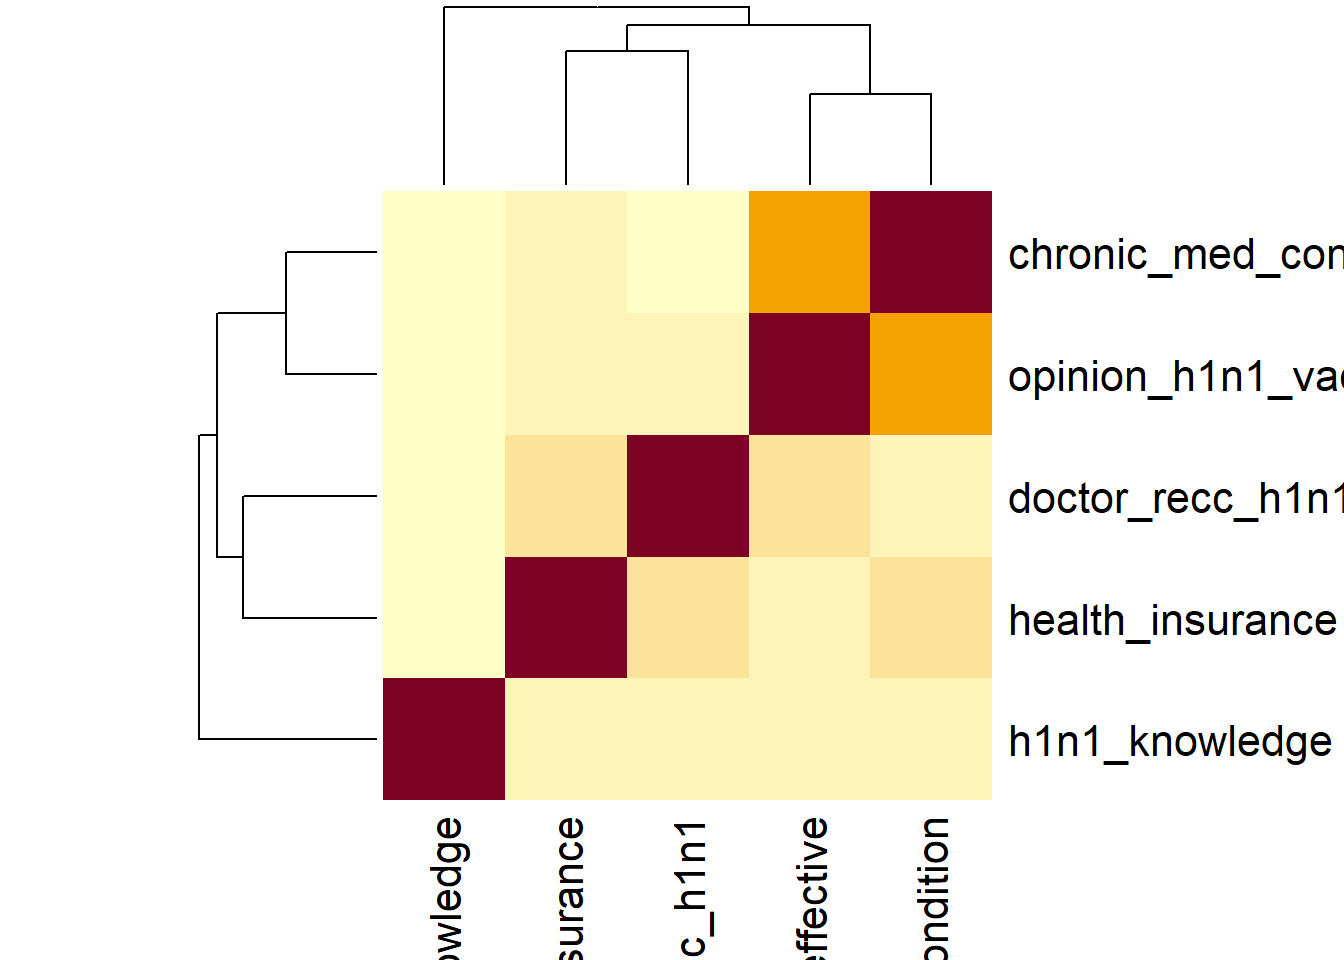
\includegraphics{RLearning_files/figure-latex/unnamed-chunk-83-1.pdf}

根据缺失相关性矩阵,\passthrough{\lstinline!opinion\_h1n1\_vacc\_effective!} 与 \passthrough{\lstinline!chronic\_med\_condition!} 缺失相关性较大。

综上,在案例中,变量之间的存在部分相关性,考虑为MAR。

其他数据缺失关系分析,可参考附录\passthrough{\lstinline!数据的预处理基础!}。

\hypertarget{ux7f3aux5931ux503cux5904ux7406}{%
\subsubsection{缺失值处理}\label{ux7f3aux5931ux503cux5904ux7406}}

缺失值一般有三种方式:

\begin{itemize}
\tightlist
\item
  将缺失值作为变量值使用。比如在民意调查中,当选民不投票时,可以将缺失值处理为``无法确定''。
\item
  删除数据。主要有删除样本值和删除特征值。但可能会损失掉一些有用信息。
\item
  插补法。如均值/中位数/同类均值插补(数值变量),众数插补(类别变量),手动插补(根据主观理解),多重插补等。
\end{itemize}

以下我们主要介绍删除法和插补法:

\hypertarget{ux5220ux9664ux6cd5}{%
\paragraph{删除法}\label{ux5220ux9664ux6cd5}}

行删除,可以直接用\passthrough{\lstinline!complete.cases()!}或\passthrough{\lstinline!na.omit()!}来过滤掉数据集中所有缺失行。

\begin{lstlisting}[language=R]
h1n1_data_row_del1 <- h1n1_data[!complete.cases(h1n1_data), ]
h1n1_data_row_del2 <- na.omit(h1n1_data)
\end{lstlisting}

列删除,一般对于缺失率极高又没有太大作用的特征值,我们直接删除,如可以用\passthrough{\lstinline!dataset[,-5]!}去掉第五列,或\passthrough{\lstinline!subset(dataset, select = -c(col1, col2))!}去掉列col1和列col2。

比如,我们把\passthrough{\lstinline!health\_insurance!}变量删除。

\begin{lstlisting}[language=R]
h1n1_data_col_del1 <- subset(h1n1_data, select = -c(health_insurance))
\end{lstlisting}

\hypertarget{ux7b80ux5355ux63d2ux8865ux6cd5}{%
\paragraph{简单插补法}\label{ux7b80ux5355ux63d2ux8865ux6cd5}}

注意在空值插补的时候,要区分类别变量与数值变量,均值插补不适用于类别变量。我们这里随机选择了一个变量演示\passthrough{\lstinline!impute()!}函数用法,在实际插补的时候,请大家根据情况进行选择。

\begin{lstlisting}[language=R]
h1n1_data_sim_imp <- h1n1_data
h1n1_data_sim_imp$h1n1_knowledge <- impute(h1n1_data_sim_imp$h1n1_knowledge, 1) # 填充特定值
h1n1_data_sim_imp$h1n1_knowledge <- impute(h1n1_data_sim_imp$h1n1_knowledge, median) # 插补中位数
h1n1_data_sim_imp$h1n1_knowledge <- impute(h1n1_data_sim_imp$h1n1_knowledge, mean) # 插补均值
\end{lstlisting}

\hypertarget{ux62dfux5408ux63d2ux8865ux6cd5}{%
\paragraph{拟合插补法}\label{ux62dfux5408ux63d2ux8865ux6cd5}}

利用有监督的机器学习方法,比如回归、最邻近、随机森林、支持向量机等模型,对缺失值作预测。

\hypertarget{ux591aux91cdux63d2ux8865ux6cd5}{%
\paragraph{多重插补法}\label{ux591aux91cdux63d2ux8865ux6cd5}}

多重插补(MI)是一种基于重复模拟的处理缺失值的方法。其思想来源于贝叶斯估计,认为待插补的值是随机的,它的值来自于已观测到的值。具体实践上通常是估计出待插补的值,然后再加上不同的噪声,形成多组可选插补值(通常是3到10个)。根据某种选择依据,选取最合适的插补值。与单个插补(例如均值)相比,创建多个插补可解决缺失值的不确定性。 R中可利用\passthrough{\lstinline!Amelia!}、\passthrough{\lstinline!mice!}和\passthrough{\lstinline!mi!}包来执行这些操作。

本节中,我们将用案例介绍mice包(通过链式方程进行的多元插补)提供的方法。使用mice生成m个完整的插补数据集。然后利用\passthrough{\lstinline!with-pool!}的方法来评估选择哪一个数据集。首先使用\passthrough{\lstinline!with()!}函数依次对每个完整数据集应用统计模型如lm,glm等,用\passthrough{\lstinline!summary()!}输出数据集检验,看某数据集是否合格。接下来\passthrough{\lstinline!pool()!}函数把5个回归模型汇总,用\passthrough{\lstinline!summary()!}输出汇总数据集检验,查看整体插补方法是否合格。检验结果分析可参考附录\passthrough{\lstinline!mice检验结果解释!}

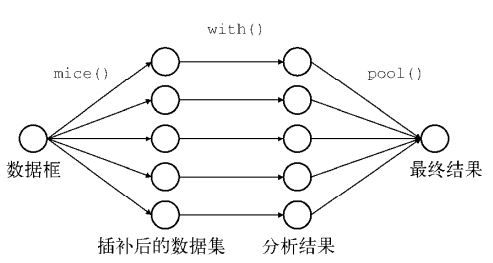
\includegraphics[width=0.6\textwidth,height=\textheight]{./image/task02_mice.jpg}

\begin{lstlisting}[language=R]
# 先处理下数据,把数据集中一些类别变量转换回来

# imp是一个包含m个插补数据集的列表对象,同时还含有完成插补过程的信息。
# 参数m的默认值为5,这里我们将m设为4,生成4个无缺失数据集
# 参数method, 对于每个变量的拟合,可以指定所用的拟合方法,method传入的参数可以是一个具体方法,也可以为不同列指定具体方法,具体方法选择可参考附录mice使用文档。这里我们使用默认值。
imp <- mice(h1n1_data, m = 4, seed = 122, printFlag = FALSE)

# 查看变量h1n1_knowledge在几个插补数据集中的插补结果
# imp$imp$h1n1_knowledge

# 查看每个变量所用的插补方法
# imp$method

# 设定应用于m个插补数据集的统计分析方法。方法包括做线性回归模型的lm()函数、做广义线性模型的glm()函数、做广义可加模型的gam(),做负二项模型的nbrm()函数
fit <- with(imp, lm(h1n1_vaccine ~ h1n1_knowledge + doctor_recc_h1n1 + chronic_med_condition + health_insurance + opinion_h1n1_vacc_effective))

# 输出每个数据集检验
print.data.frame(summary(fit), digits = 4)
\end{lstlisting}

\begin{lstlisting}
##                           term estimate std.error statistic    p.value  nobs
## 1                  (Intercept) -0.30492  0.010809   -28.209 1.557e-172 26707
## 2               h1n1_knowledge  0.03645  0.003661     9.956  2.596e-23 26707
## 3             doctor_recc_h1n1  0.34604  0.005568    62.147  0.000e+00 26707
## 4        chronic_med_condition  0.03033  0.005015     6.048  1.485e-09 26707
## 5             health_insurance  0.07826  0.006754    11.587  5.706e-31 26707
## 6  opinion_h1n1_vacc_effective  0.08317  0.002245    37.054 4.116e-293 26707
## 7                  (Intercept) -0.30718  0.010901   -28.179 3.509e-172 26707
## 8               h1n1_knowledge  0.03689  0.003683    10.016  1.429e-23 26707
## 9             doctor_recc_h1n1  0.33876  0.005563    60.893  0.000e+00 26707
## 10       chronic_med_condition  0.02972  0.005031     5.907  3.521e-09 26707
## 11            health_insurance  0.07776  0.006957    11.178  6.028e-29 26707
## 12 opinion_h1n1_vacc_effective  0.08385  0.002258    37.128 2.986e-294 26707
## 13                 (Intercept) -0.30981  0.010830   -28.607 2.603e-177 26707
## 14              h1n1_knowledge  0.03666  0.003679     9.965  2.386e-23 26707
## 15            doctor_recc_h1n1  0.33489  0.005557    60.262  0.000e+00 26707
## 16       chronic_med_condition  0.02948  0.005035     5.855  4.814e-09 26707
## 17            health_insurance  0.08090  0.006742    12.000  4.334e-33 26707
## 18 opinion_h1n1_vacc_effective  0.08415  0.002258    37.272 1.851e-296 26707
## 19                 (Intercept) -0.30608  0.010910   -28.055 1.047e-170 26707
## 20              h1n1_knowledge  0.03702  0.003685    10.046  1.056e-23 26707
## 21            doctor_recc_h1n1  0.33370  0.005564    59.970  0.000e+00 26707
## 22       chronic_med_condition  0.02969  0.005040     5.891  3.877e-09 26707
## 23            health_insurance  0.07557  0.006896    10.959  6.877e-28 26707
## 24 opinion_h1n1_vacc_effective  0.08423  0.002259    37.278 1.490e-296 26707
\end{lstlisting}

\begin{lstlisting}[language=R]
# 包含m个统计分析平均结果的列表对象
pooled <- pool(fit)

# 这是一个总体评估结果
pooled
\end{lstlisting}

\begin{lstlisting}
## Class: mipo    m = 4 
##                          term m    estimate         ubar            b
## 1                 (Intercept) 4 -0.30699871 1.179991e-04 4.368721e-06
## 2              h1n1_knowledge 4  0.03675472 1.352049e-05 6.410610e-08
## 3            doctor_recc_h1n1 4  0.33834805 3.094965e-05 3.095473e-05
## 4       chronic_med_condition 4  0.02980518 2.530162e-05 1.342220e-07
## 5            health_insurance 4  0.07812323 4.675346e-05 4.779575e-06
## 6 opinion_h1n1_vacc_effective 4  0.08385005 5.085296e-06 2.294296e-07
##              t dfcom           df         riv      lambda         fmi
## 1 1.234600e-04 26701  1446.448456 0.046279160 0.044232134 0.045550936
## 2 1.360062e-05 26701 20305.470346 0.005926755 0.005891836 0.005989737
## 3 6.964306e-05 26701     9.710629 1.250205046 0.555596055 0.625522404
## 4 2.546940e-05 26701 19168.975299 0.006631097 0.006587415 0.006691047
## 5 5.272792e-05 26701   231.386715 0.127786668 0.113307482 0.120873547
## 6 5.372083e-06 26701  1010.568516 0.056395341 0.053384693 0.055252579
\end{lstlisting}

\begin{lstlisting}[language=R]
# 这里修改action的参数(范围1-m),选择一个数据集作为我们已填充完成的数据集
h1n1_data_complete <- complete(imp, action = 2)
\end{lstlisting}

\hypertarget{ux5f02ux5e38ux503cux8bc6ux522bux4e0eux5904ux7406}{%
\subsection{异常值识别与处理}\label{ux5f02ux5e38ux503cux8bc6ux522bux4e0eux5904ux7406}}

\hypertarget{ux5f02ux5e38ux503cux8bc6ux522b}{%
\subsubsection{异常值识别}\label{ux5f02ux5e38ux503cux8bc6ux522b}}

本节的异常值指离群点。为了让数据统计或数据建模更加准确,我们通常会识别并对处理一些离群点。有些模型会对异常值较敏感,参考附录\passthrough{\lstinline!什么样的模型对缺失值更敏感?!}。
总的来说,有几种常用方法,包括可视化图形分布识别(箱线图)、z-score识别、局部异常因子法(LOF法)、聚类法等。

我们这里用波士顿房价数据集来演示一下异常值识别的处理过程。

\hypertarget{ux53efux89c6ux5316ux56feux5f62ux5206ux5e03}{%
\subsubsection{可视化图形分布}\label{ux53efux89c6ux5316ux56feux5f62ux5206ux5e03}}

首先是可视化图形分布识别,将数值型变量筛选出来,用boxlpot看看分布。

\begin{lstlisting}[language=R]
# 提取数值字段
nums <- unlist(lapply(BostonHousing, is.numeric))
nums_data <- BostonHousing[, nums]

# 数据变形
nums_data.new <- nums_data %>%
  as.data.frame() %>%
  mutate(Cell = rownames(.)) %>%
  gather(., key = colname, value = "value", -Cell)

# 用ggplot画出箱线图
ggplot(data = nums_data.new, aes(x = colname, y = value)) +
  geom_boxplot(aes(1)) +
  facet_wrap(~colname, scales = "free") +
  theme_grey() +
  labs(title = "Outlier Detection On Numeric Data By Boxplot", x = "Numeric Columns", y = "") +
  theme(legend.position = "top") +
  theme_bw()
\end{lstlisting}

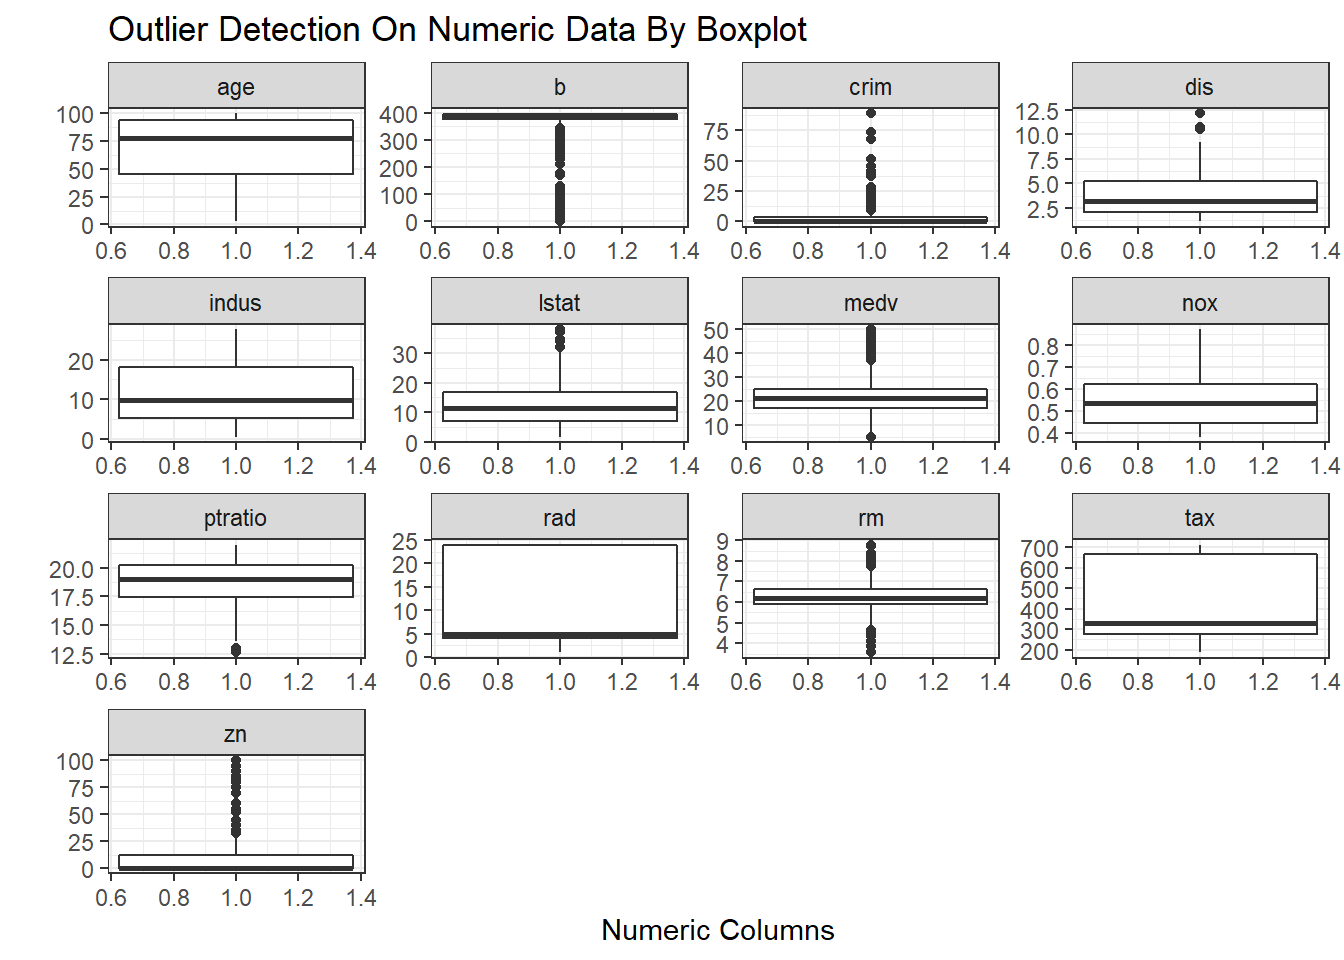
\includegraphics{RLearning_files/figure-latex/unnamed-chunk-88-1.pdf}

通过可视化分布,可以选择剔除一些不合理的离群值,比如在数据集中将dis\textgreater10.0的数据剔除。

\hypertarget{z-score}{%
\subsubsection{z-score}\label{z-score}}

z-score是一种一维或低维特征空间中参数异常检测方法。它假定数据是高斯分布,异常值是分布尾部的数据点,因此远离数据的平均值。一般将z-score低于-3或高于3的数据看成是异常值。

\begin{lstlisting}[language=R]
# 定义一个识别异常点的函数,x是输入数据(matrix或df),zs是异常临界值,z-score超过zs的被识别为异常点
outliers <- function(x, zs) {
  temp <- abs(apply(x, 1, scale))
  return(x[temp > zs])
}
# 打印出z-score<3的值
outliers(nums_data, 3)
\end{lstlisting}

\begin{lstlisting}
##  [1]   7.380   0.700   0.573   5.889  17.400  20.200 392.400 396.900 396.900
## [10] 393.680 396.900 368.570 396.900 377.730 375.330 396.900 391.980 100.630
## [19] 388.520 255.230 374.680 392.680 395.770  12.430  11.280  27.710  10.210
## [28]   6.860   9.880   9.620   4.210  13.000  25.410  16.900  29.550   6.360
## [37]   4.850   4.700   4.610  13.270   2.960  24.560  19.370  14.100  14.330
## [46]  22.800  33.400
\end{lstlisting}

\hypertarget{ux5c40ux90e8ux5f02ux5e38ux56e0ux5b50ux6cd5}{%
\subsubsection{局部异常因子法}\label{ux5c40ux90e8ux5f02ux5e38ux56e0ux5b50ux6cd5}}

局部异常因子法(LOF),是一种无监督的离群检测方法,是基于密度的离群点检测方法中一个比较有代表性的算法。适用于在中等高维数据集上执行异常值检测。

\begin{lstlisting}[language=R]
# k是计算局部异常因子所需要判断异常点周围的点的个数
outlier_score <- lof(data = nums_data, k = 5)

# 绘制异常值得分的直方分布图
hist(outlier_score, col = "#8ac6d1")
\end{lstlisting}

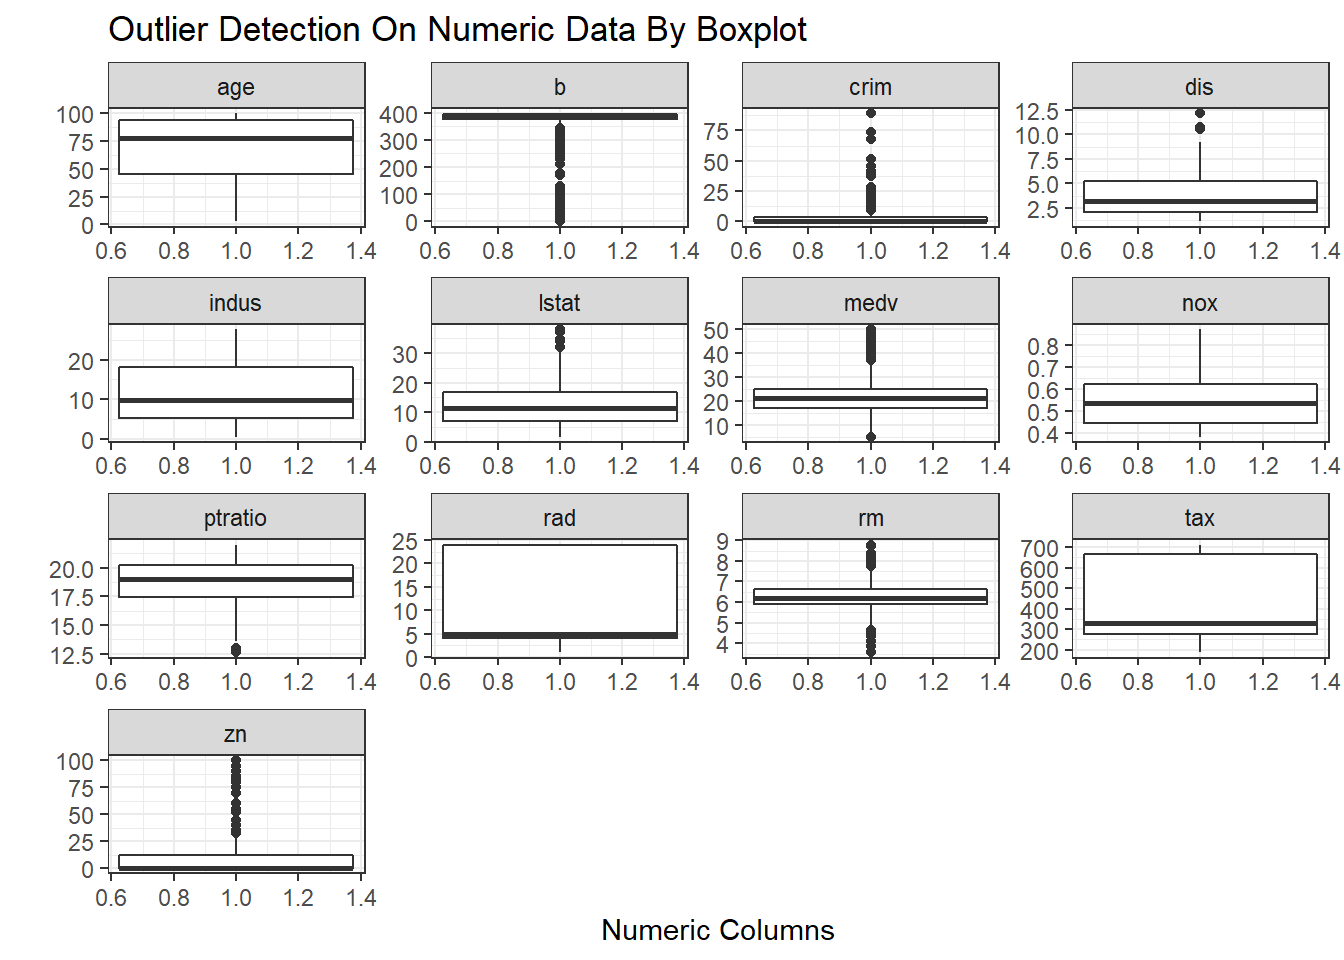
\includegraphics{RLearning_files/figure-latex/unnamed-chunk-90-1.pdf}

\begin{lstlisting}[language=R]
# 排序,挑出得分排前五的数据(找到索引)作为异常值
names(outlier_score) <- 1:nrow(nums_data)
sort(outlier_score, decreasing = TRUE)[1:5]
\end{lstlisting}

\begin{lstlisting}
##      489      493      381      492      406 
## 5.133201 4.534088 4.529170 3.732775 3.559666
\end{lstlisting}

\hypertarget{ux5f02ux5e38ux503cux5904ux7406}{%
\subsubsection{异常值处理}\label{ux5f02ux5e38ux503cux5904ux7406}}

首先需要确定是否是真的异常值,有些值虽然离群,但其实并不是异常值,处理掉反而会影响后续任务的准确性。 如果确定需要处理,可以参考缺失值的处理方式进行处理。

\hypertarget{ux7279ux5f81ux7f16ux7801}{%
\subsection{特征编码}\label{ux7279ux5f81ux7f16ux7801}}

为什么要进行特征编码?我们拿到的原始数据中,一般会有一些类别变量,但是在统计或机器学习中,我们通常需要把类别变量转化为数值型变量,才能应用于一些方法中。

\hypertarget{ux72ecux70edux7f16ux7801ux54d1ux7f16ux7801}{%
\subsubsection{独热编码/哑编码}\label{ux72ecux70edux7f16ux7801ux54d1ux7f16ux7801}}

One-hot encoding 和 dummy,是将类别变量扩充为多个只显示1,0的变量,每个变量代表原类别变量中的一个类。 注意他们之间的区别:\url{https://www.cnblogs.com/lianyingteng/p/7792693.html}

\begin{itemize}
\tightlist
\item
  优点:解决了分类器不好处理分类数据的问题,在一定程度上也起到了扩充特征的作用。它的值只有0和1,不同的类型存储在垂直的空间。\\
\item
  缺点:当类别的数量很多时,特征空间会变得非常大,容易造成维度灾难。(为避免维度灾难,后续可以考虑降维处理)
\end{itemize}

R里面有很多现成的转化编码的包,我们这里使用了\passthrough{\lstinline!dummy\_cols()!}函数做演示,可以看到原来的类别类型字段,已经扩充为多个0,1编码的字段。

\begin{lstlisting}[language=R]
h1n1_data_dummy <- dummy_cols(subset(h1n1_data_complete, select = c(age_group)), select_columns = c("age_group"))
head(h1n1_data_dummy)
\end{lstlisting}

\begin{lstlisting}
##       age_group age_group_18 - 34 Years age_group_35 - 44 Years
## 1 55 - 64 Years                       0                       0
## 2 35 - 44 Years                       0                       1
## 3 18 - 34 Years                       1                       0
## 4     65+ Years                       0                       0
## 5 45 - 54 Years                       0                       0
## 6     65+ Years                       0                       0
##   age_group_45 - 54 Years age_group_55 - 64 Years age_group_65+ Years
## 1                       0                       1                   0
## 2                       0                       0                   0
## 3                       0                       0                   0
## 4                       0                       0                   1
## 5                       1                       0                   0
## 6                       0                       0                   1
\end{lstlisting}

\hypertarget{ux6807ux7b7eux7f16ux7801}{%
\subsubsection{标签编码}\label{ux6807ux7b7eux7f16ux7801}}

标签编码(Label Encoder)是将类别变量转换成连续的数值型变量,通常对有序的变量进行标签编码,既保留了顺序信息,也节约了空间(不会扩充变量)

R里有一个特殊的结构factor(factor是有序的分类变量),我们这里可以利用factor来做标签编码。首先根据实际情况设置factor的类别顺序,然后直接用\passthrough{\lstinline!as.numeric()!}转化为数字。

\begin{lstlisting}[language=R]
h1n1_data_complete_lab_encoder <- h1n1_data_complete
h1n1_data_complete_lab_encoder$income_poverty_lab_encoder <- as.numeric(factor(h1n1_data_complete_lab_encoder$income_poverty, levels = c("Below Poverty", "<= $75,000, Above Poverty", "> $75,000")))
head(subset(h1n1_data_complete_lab_encoder, select = c(income_poverty, income_poverty_lab_encoder)))
\end{lstlisting}

\begin{lstlisting}
##              income_poverty income_poverty_lab_encoder
## 1             Below Poverty                          1
## 2             Below Poverty                          1
## 3 <= $75,000, Above Poverty                          2
## 4             Below Poverty                          1
## 5 <= $75,000, Above Poverty                          2
## 6 <= $75,000, Above Poverty                          2
\end{lstlisting}

\hypertarget{ux624bux52a8ux7f16ux7801}{%
\subsubsection{手动编码}\label{ux624bux52a8ux7f16ux7801}}

比如,当某一个特征中有很多类别,我们认为某些类别可以合为一类,可以用\passthrough{\lstinline!case\_when()!}函数手动处理。

\begin{lstlisting}[language=R]
h1n1_data_manual <- subset(h1n1_data_complete, select = c(age_group))
h1n1_data_manual$age_group_manual <- case_when(
  h1n1_data_manual$age_group %in% c("18 - 34 Years") ~ 1,
  h1n1_data_manual$age_group %in% c("35 - 44 Years", "45 - 54 Years", "55 - 64 Years") ~ 2,
  h1n1_data_manual$age_group %in% c("65+ Years") ~ 3
)
head(h1n1_data_manual)
\end{lstlisting}

\begin{lstlisting}
##       age_group age_group_manual
## 1 55 - 64 Years                2
## 2 35 - 44 Years                2
## 3 18 - 34 Years                1
## 4     65+ Years                3
## 5 45 - 54 Years                2
## 6     65+ Years                3
\end{lstlisting}

\hypertarget{ux65e5ux671fux7279ux5f81ux8f6cux6362}{%
\subsubsection{日期特征转换}\label{ux65e5ux671fux7279ux5f81ux8f6cux6362}}

参考附录\passthrough{\lstinline!R语言日期时间处理!}

\hypertarget{ux89c4ux8303ux5316ux4e0eux504fux6001ux6570ux636e}{%
\subsection{规范化与偏态数据}\label{ux89c4ux8303ux5316ux4e0eux504fux6001ux6570ux636e}}

为什么要数据规范化?简单来说是为了去除数据量纲和数据大小的差异,确保数据是在同一量纲或者同一数量级下进行比较,一般用在机器学习算法之前。数据规范化又可以使用0-1规范化,Z-score等方法。
为什么要处理偏态数据?。很多模型会假设数据或参数服从正态分布。例如线性回归(linear regression),它假设误差服从正态分布。

提示:注意在测试数据与训练数据分布差别很大的情况下,对测试数据运用一些规范化方法时,可能因为数据分布不匹配而带来误差。

这里我们使用波士顿房价数据集来做演示。可以看到图中数据的偏态分布及量纲差别。

\begin{lstlisting}[language=R]
BostonHousing %>%
  keep(is.numeric) %>%
  gather() %>%
  ggplot(aes(value)) +
  facet_wrap(~key, scales = "free") +
  geom_density(color = "#348498", fill = "#8ac6d1") +
  theme_bw()
\end{lstlisting}

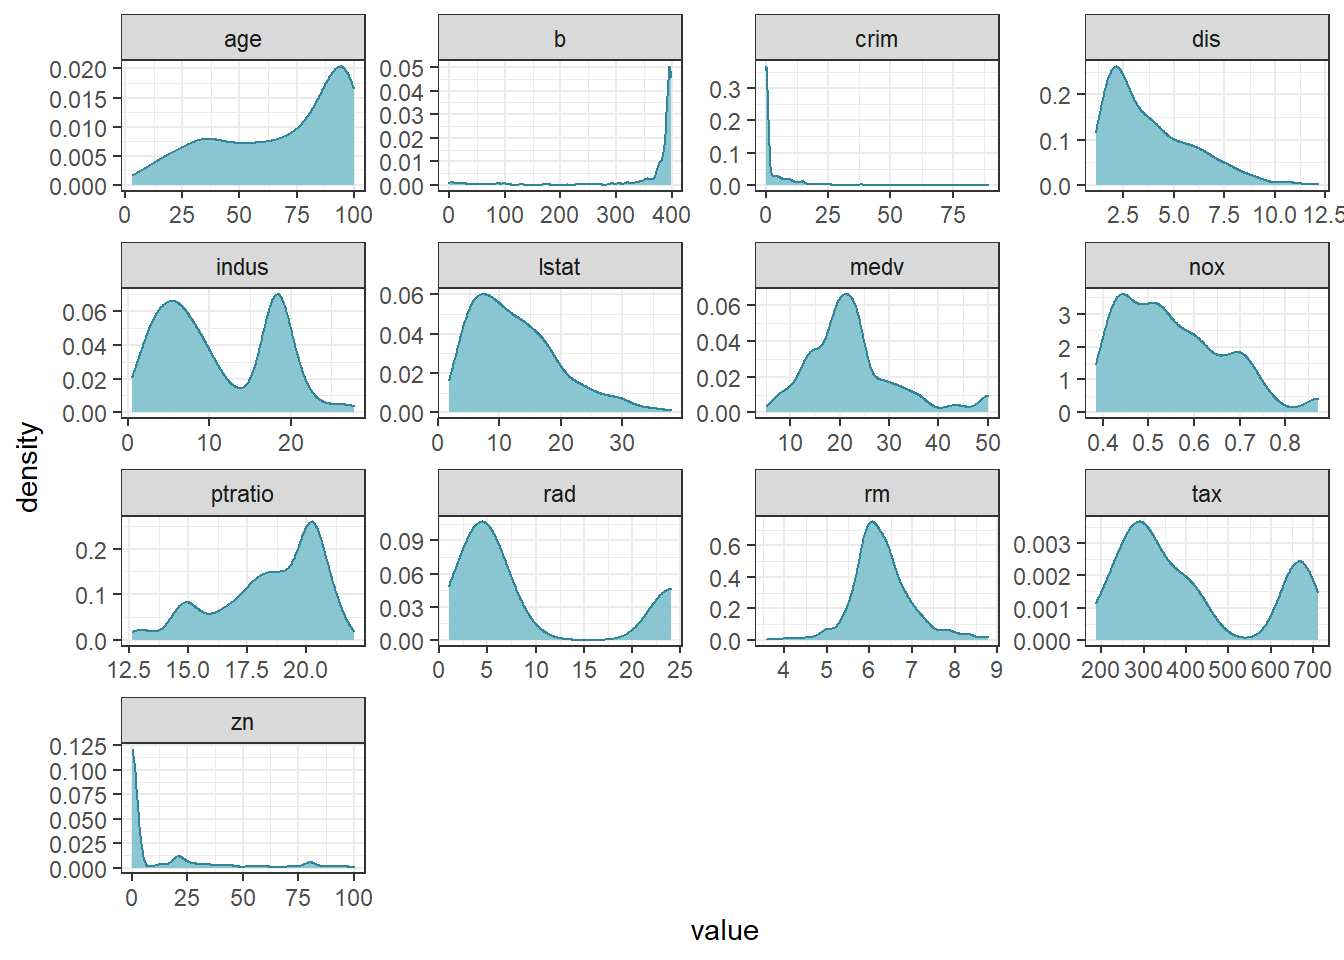
\includegraphics{RLearning_files/figure-latex/unnamed-chunk-94-1.pdf}

\hypertarget{ux89c4ux8303ux5316}{%
\subsubsection{0-1规范化}\label{ux89c4ux8303ux5316}}

0-1规范化是将原始数据缩放到{[}0,1{]}区间内,一般方法是最小最大规范的方法,公式如下:

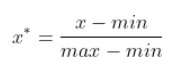
\includegraphics[width=0.2\textwidth,height=\textheight]{./image/task02_0-1norm.png}

这里用循环计算出每一列的最大最小值,再根据公式求出缩放后的数据。

\begin{lstlisting}[language=R]
nums_data_norm1 <- nums_data
for (col in names(nums_data_norm1))
{
  xmin <- min(nums_data_norm1[col])
  xmax <- max(nums_data_norm1[col])
  nums_data_norm1[col] <- (nums_data_norm1[col] - xmin) / (xmax - xmin)
}

head(nums_data_norm1)
\end{lstlisting}

\begin{lstlisting}
##           crim   zn      indus       nox        rm       age       dis
## 1 0.0000000000 0.18 0.06781525 0.3148148 0.5775053 0.6416066 0.2692031
## 2 0.0002359225 0.00 0.24230205 0.1728395 0.5479977 0.7826982 0.3489620
## 3 0.0002356977 0.00 0.24230205 0.1728395 0.6943859 0.5993821 0.3489620
## 4 0.0002927957 0.00 0.06304985 0.1502058 0.6585553 0.4418126 0.4485446
## 5 0.0007050701 0.00 0.06304985 0.1502058 0.6871048 0.5283213 0.4485446
## 6 0.0002644715 0.00 0.06304985 0.1502058 0.5497222 0.5746653 0.4485446
##          rad        tax   ptratio         b      lstat      medv
## 1 0.00000000 0.20801527 0.2872340 1.0000000 0.08967991 0.4222222
## 2 0.04347826 0.10496183 0.5531915 1.0000000 0.20447020 0.3688889
## 3 0.04347826 0.10496183 0.5531915 0.9897373 0.06346578 0.6600000
## 4 0.08695652 0.06679389 0.6489362 0.9942761 0.03338852 0.6311111
## 5 0.08695652 0.06679389 0.6489362 1.0000000 0.09933775 0.6933333
## 6 0.08695652 0.06679389 0.6489362 0.9929901 0.09602649 0.5266667
\end{lstlisting}

转换完再看一下分布,已经缩放到0-1之间了。

\begin{lstlisting}[language=R]
nums_data_norm1 %>%
  keep(is.numeric) %>%
  gather() %>%
  ggplot(aes(value)) +
  facet_wrap(~key, scales = "free") +
  geom_density(color = "#348498", fill = "#8ac6d1") +
  theme_bw()
\end{lstlisting}

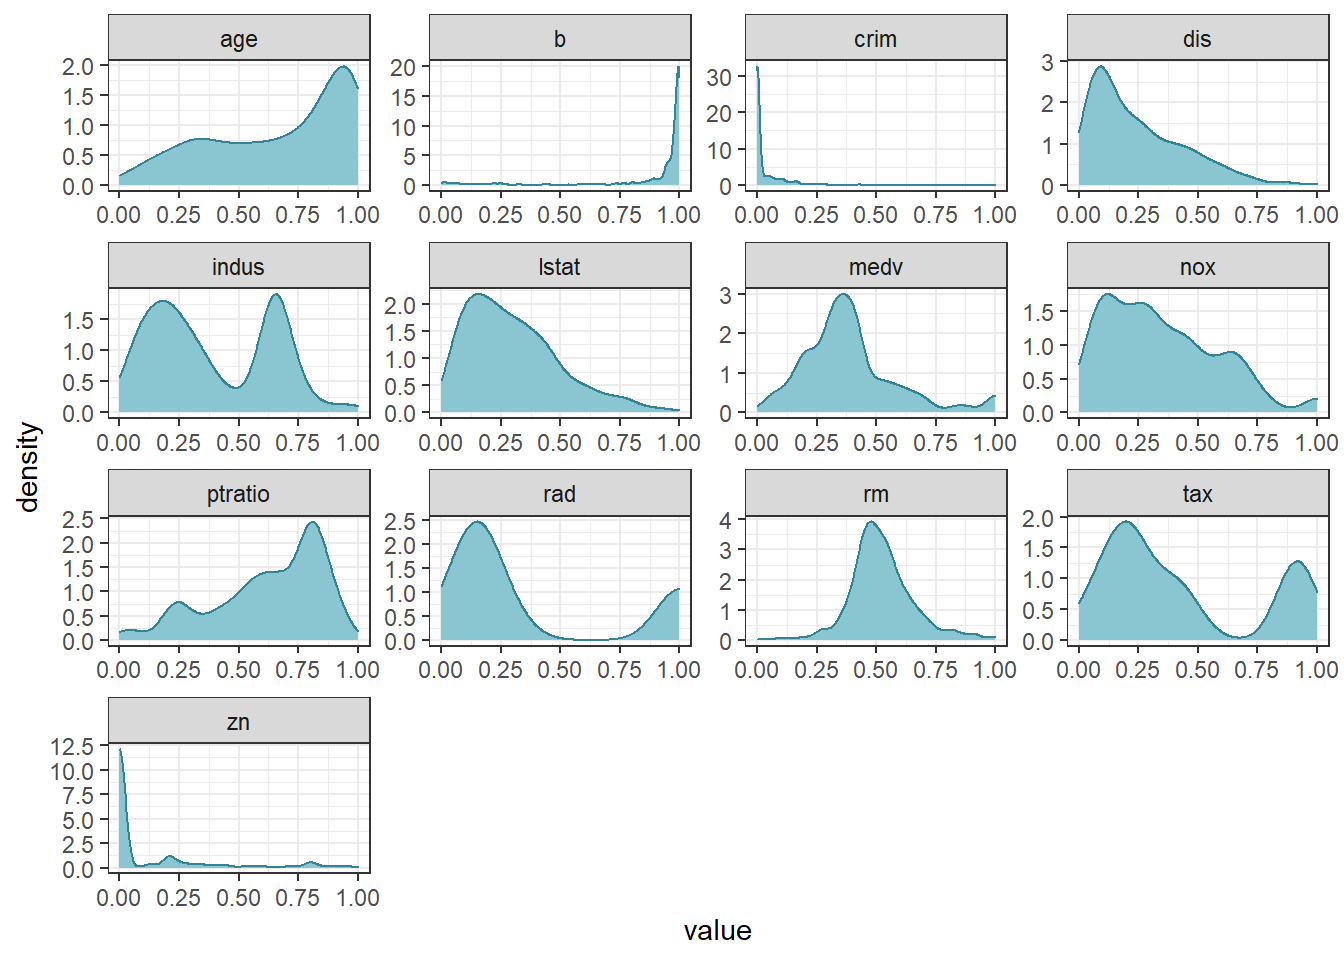
\includegraphics{RLearning_files/figure-latex/unnamed-chunk-96-1.pdf}

此外可以用dlookr包里的\passthrough{\lstinline!transform()!}函数。

\begin{lstlisting}[language=R]
nums_data_norm2 <- nums_data
nums_data_norm2$crim <- dlookr::transform(nums_data$crim, method = "minmax")
\end{lstlisting}

\hypertarget{z-scoreux6807ux51c6ux5316}{%
\subsubsection{Z-score标准化}\label{z-scoreux6807ux51c6ux5316}}

Z-score标准化是原数据减去期望再除以标准差,将数据按比例缩放,使其落入到一个小的区间内,标准化后的数据可正可负,但是一般绝对值不会太大。

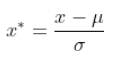
\includegraphics[width=0.15\textwidth,height=\textheight]{./image/task02_z-score.png}

R里面可以用\passthrough{\lstinline!scale()!}函数来计算z-score。也可以dlookr包里的中\passthrough{\lstinline!transform()!}函数。

\begin{lstlisting}[language=R]
nums_data_zscore <- nums_data
nums_data_zscore <- scale(nums_data_zscore)
head(nums_data_zscore)
\end{lstlisting}

\begin{lstlisting}
##         crim         zn      indus        nox        rm        age      dis
## 1 -0.4193669  0.2845483 -1.2866362 -0.1440749 0.4132629 -0.1198948 0.140075
## 2 -0.4169267 -0.4872402 -0.5927944 -0.7395304 0.1940824  0.3668034 0.556609
## 3 -0.4169290 -0.4872402 -0.5927944 -0.7395304 1.2814456 -0.2655490 0.556609
## 4 -0.4163384 -0.4872402 -1.3055857 -0.8344581 1.0152978 -0.8090878 1.076671
## 5 -0.4120741 -0.4872402 -1.3055857 -0.8344581 1.2273620 -0.5106743 1.076671
## 6 -0.4166314 -0.4872402 -1.3055857 -0.8344581 0.2068916 -0.3508100 1.076671
##          rad        tax    ptratio         b      lstat       medv
## 1 -0.9818712 -0.6659492 -1.4575580 0.4406159 -1.0744990  0.1595278
## 2 -0.8670245 -0.9863534 -0.3027945 0.4406159 -0.4919525 -0.1014239
## 3 -0.8670245 -0.9863534 -0.3027945 0.3960351 -1.2075324  1.3229375
## 4 -0.7521778 -1.1050216  0.1129203 0.4157514 -1.3601708  1.1815886
## 5 -0.7521778 -1.1050216  0.1129203 0.4406159 -1.0254866  1.4860323
## 6 -0.7521778 -1.1050216  0.1129203 0.4101651 -1.0422909  0.6705582
\end{lstlisting}

转换完再看一下分布,数据缩放后在0周围的一个小区间了。

\begin{lstlisting}[language=R]
data.frame(nums_data_zscore) %>%
  keep(is.numeric) %>%
  gather() %>%
  ggplot(aes(value)) +
  facet_wrap(~key, scales = "free") +
  geom_density(color = "#348498", fill = "#8ac6d1") +
  theme_bw()
\end{lstlisting}

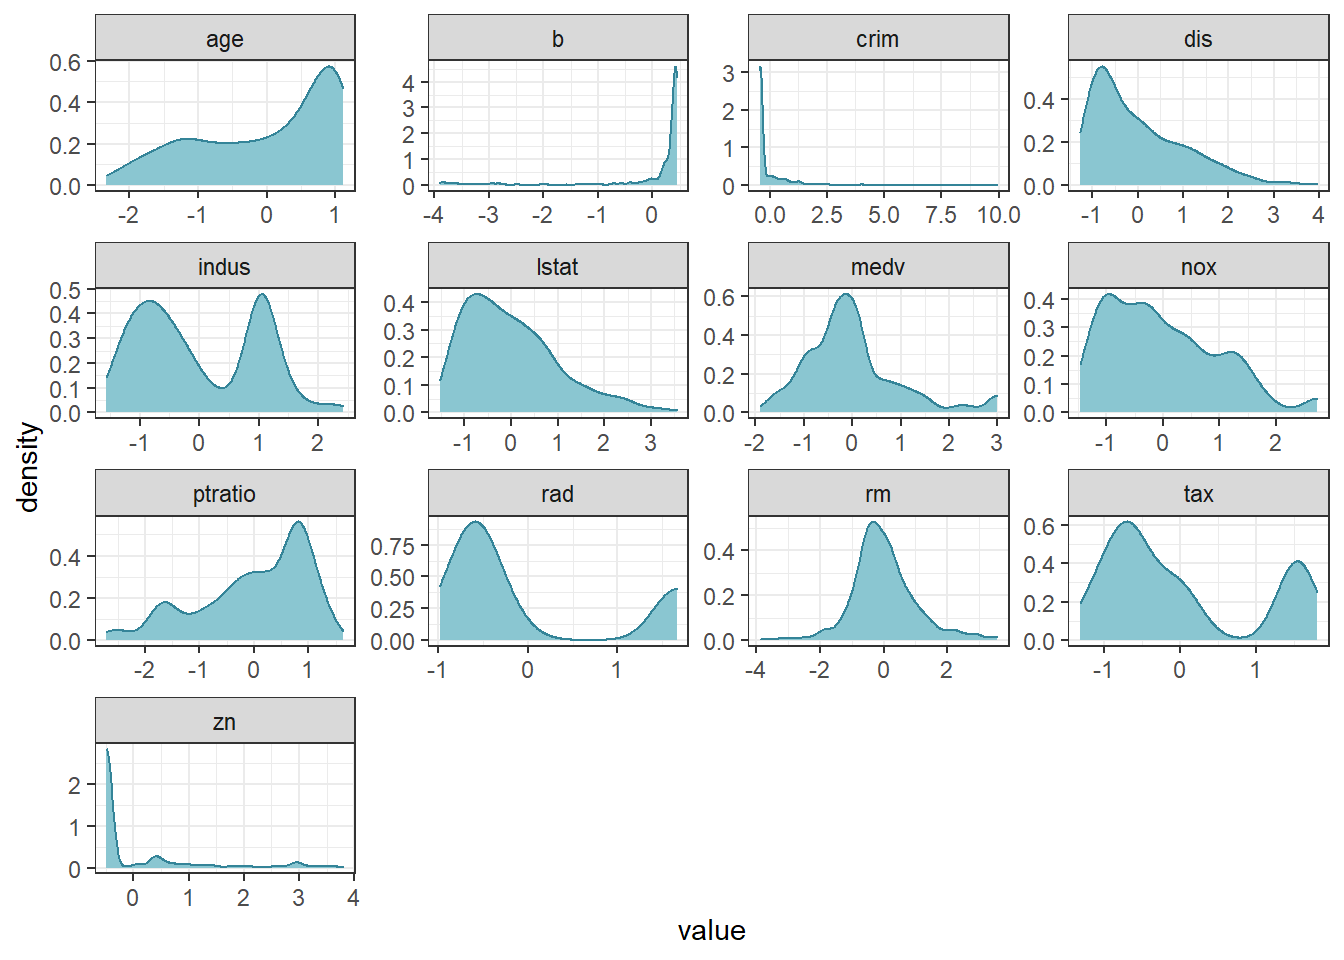
\includegraphics{RLearning_files/figure-latex/unnamed-chunk-99-1.pdf}

\hypertarget{ux5bf9ux6570ux8f6cux6362log-transform}{%
\subsubsection{对数转换(log transform)}\label{ux5bf9ux6570ux8f6cux6362log-transform}}

使用对数转换也是一种常见的处理偏斜特征的方法,但要注意原数据中不能含有负值。此外为了避免0值,我们通常使用log1p,公式为\passthrough{\lstinline!lg(x+1)!}。可以直接用dlookr包里的\passthrough{\lstinline!transform()!}函数,一般结合mutate函数一起使用。

\begin{lstlisting}[language=R]
# 直接公式转换
nums_data_log1p1 <- log(nums_data + 1)

# 用transform()函数
nums_data_log1p2 <- nums_data
nums_data_log1p2$b <- dlookr::transform(nums_data_log1p2$b, method = "log+1")
\end{lstlisting}

转换完再看一下分布,大多变量转换后接近正态分布了。但是这里要特别注意离散数据。

\begin{lstlisting}[language=R]
nums_data_log1p1 %>%
  keep(is.numeric) %>%
  gather() %>%
  ggplot(aes(value)) +
  facet_wrap(~key, scales = "free") +
  geom_density(color = "#348498", fill = "#8ac6d1") +
  theme_bw()
\end{lstlisting}

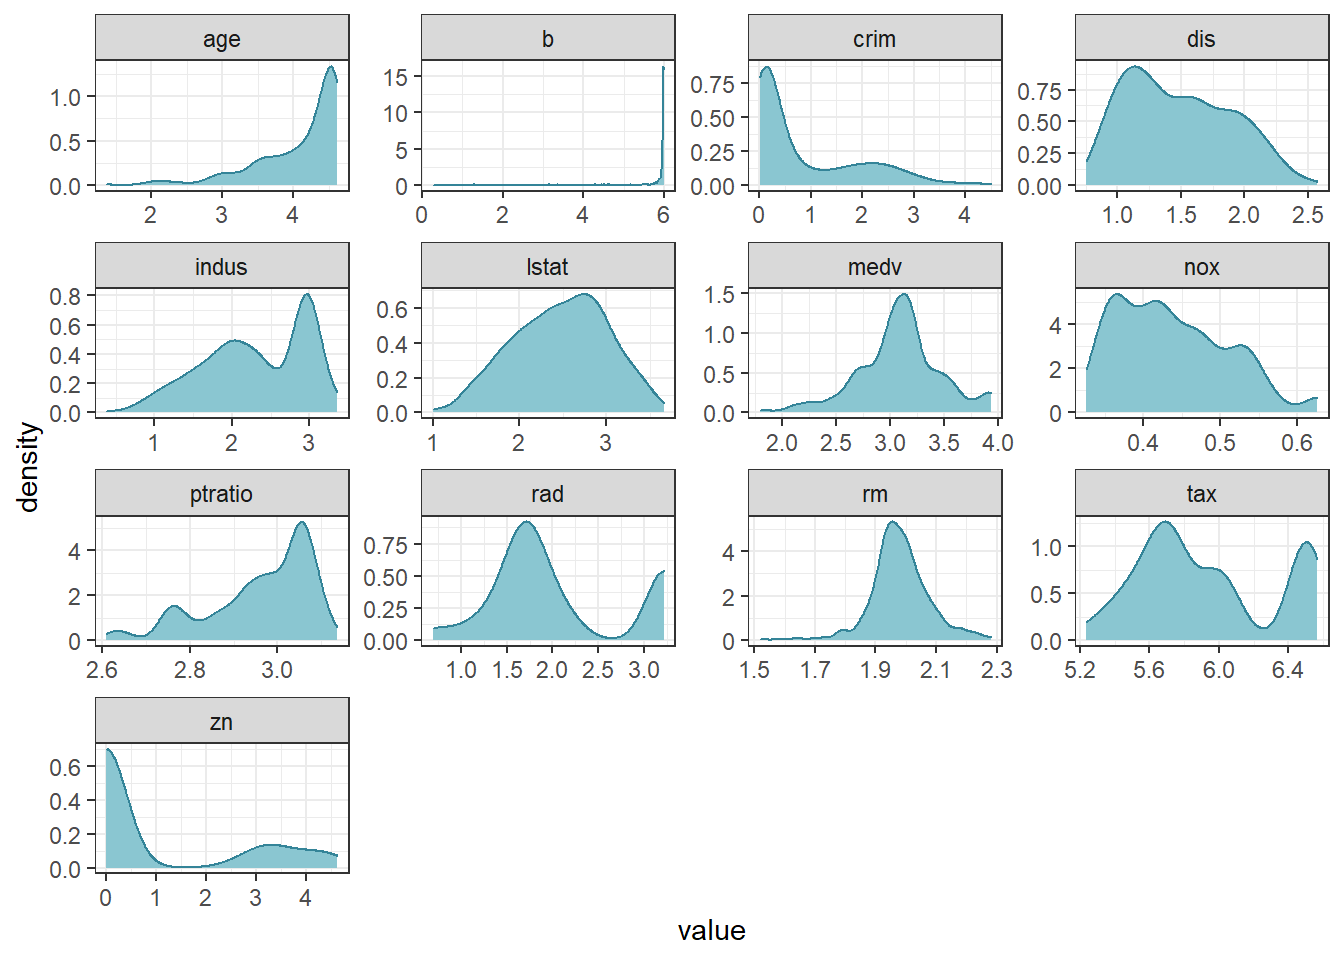
\includegraphics{RLearning_files/figure-latex/unnamed-chunk-101-1.pdf}

\hypertarget{box-cox}{%
\subsubsection{Box-Cox}\label{box-cox}}

Box-Cox变换是Box和Cox在1964年提出的一种广义幂变换方法,在变换后可以一定程度上减小不可观测的误差和预测变量的相关性,在机器学习中经常用来处理偏态分布。其一个显著优点是通过求变换参数来确定变换形式,而这个过程完全基于数据本身而无须任何先验信息,这无疑比凭经验或通过尝试而选用对数、平方根等变换方式要客观和精确。计算公式如下:

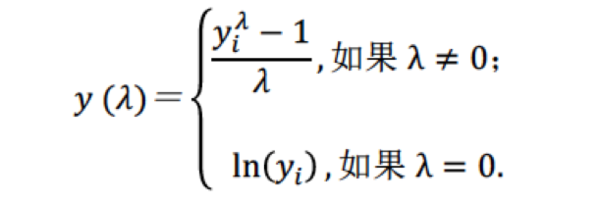
\includegraphics[width=0.4\textwidth,height=\textheight]{./image/task02_boxcox.png}

示例参考附录\passthrough{\lstinline!基于R语言进行Box-Cox变换!}

\hypertarget{ux5c0fux62d3ux5c55}{%
\subsection{小拓展}\label{ux5c0fux62d3ux5c55}}

R语言中,mutate 类似于SQL中,根据表的现有变量,生成新变量。使用mutate集中处理变量转换,代码显示较整洁。

\begin{lstlisting}[language=R]
h1n1_data_de <- h1n1_data_complete %>%
  to_dummy(education, suffix = "label") %>%
  bind_cols(h1n1_data_complete) %>%
  mutate(
    # 标签编码(label encoder)
    sex = as.factor(as.numeric(factor(sex))),
    income_poverty = (as.numeric(factor(
      income_poverty,
      levels = c(
        "Below Poverty",
        "<= $75,000, Above Poverty",
        "> $75,000"
      )
    ))),
    # 手动编码
    age_group = as.factor(
      case_when(
        age_group %in% c("18 - 34 Years") ~ 1,
        age_group %in% c("35 - 44 Years", "45 - 54 Years", "55 - 64 Years") ~ 2,
        age_group %in% c("65+ Years") ~ 3
      )
    ),
    # 标准化
    across(
      c(
        "h1n1_knowledge",
        "doctor_recc_h1n1",
        "chronic_med_condition",
        "opinion_h1n1_vacc_effective",
        "age_group",
        "income_poverty"
      ),
      ~ scale(as.numeric(.x))
    )
  ) %>%
  dplyr::select(-one_of("education", "education_"))

head(h1n1_data_de)
\end{lstlisting}

\begin{lstlisting}
##   education_< 12 Years education_12 Years education_College Graduate
## 1                    1                  0                          0
## 2                    0                  1                          0
## 3                    0                  0                          1
## 4                    0                  1                          0
## 5                    0                  0                          0
## 6                    0                  1                          0
##   education_Some College respondent_id h1n1_knowledge doctor_recc_h1n1
## 1                      0             0     -2.0416901       -0.5258839
## 2                      0             1      1.1935904       -0.5258839
## 3                      0             2     -0.4240499       -0.5258839
## 4                      0             3     -0.4240499       -0.5258839
## 5                      1             4     -0.4240499       -0.5258839
## 6                      0             5     -0.4240499       -0.5258839
##   chronic_med_condition health_insurance opinion_h1n1_vacc_effective
## 1            -0.6284091                1                  -0.8439071
## 2            -0.6284091                1                   1.1407906
## 3             1.5912605                1                  -0.8439071
## 4             1.5912605                1                  -0.8439071
## 5            -0.6284091                0                  -0.8439071
## 6            -0.6284091                1                   1.1407906
##     age_group sex income_poverty h1n1_vaccine
## 1 -0.09109418   1     -1.8905904            0
## 2 -0.09109418   2     -1.8905904            0
## 3 -1.58547517   2     -0.2945789            0
## 4  1.40328681   1     -1.8905904            0
## 5 -0.09109418   1     -0.2945789            0
## 6  1.40328681   2     -0.2945789            0
\end{lstlisting}

注意在机器学习中,尽量在数据集划分后,分别在训练集与验证集、测试集上进行数据清洗,避免数据泄露。R中的数据集划分方法参考附录\passthrough{\lstinline!R中数据集分割!}。

\hypertarget{ux601dux8003ux4e0eux7ec3ux4e60}{%
\subsection{思考与练习}\label{ux601dux8003ux4e0eux7ec3ux4e60}}

看完了本节数据清洗与准备,尝试着选取一个完整的数据集(从本节中选取或使用自己的数据集),来做一次清洗吧!

\hypertarget{ux9644ux5f55ux53c2ux8003ux8d44ux6599}{%
\subsection*{附录:参考资料}\label{ux9644ux5f55ux53c2ux8003ux8d44ux6599}}


\hypertarget{ux7406ux8bbaux8d44ux6599}{%
\subsubsection*{理论资料}\label{ux7406ux8bbaux8d44ux6599}}


\textbf{数据的预处理基础:} 如何处理缺失值 \url{https://cloud.tencent.com/developer/article/1626004}

\textbf{多重插补法:} 处理缺失值之多重插补(Multiple Imputation)\url{https://zhuanlan.zhihu.com/p/36436260}

\textbf{异常值检测:} R语言--异常值检测 \url{https://blog.csdn.net/kicilove/article/details/76260350}

\textbf{异常值检测之LOF:} 异常检测算法之局部异常因子算法-Local Outlier Factor(LOF) \url{https://blog.csdn.net/BigData_Mining/article/details/102914342}

\textbf{规范化:} 规范化、标准化、归一化、正则化 \url{https://blog.csdn.net/u014381464/article/details/81101551}

\textbf{什么样的模型对缺失值更敏感?:} \url{https://blog.csdn.net/zhang15953709913/article/details/88717220}

\hypertarget{rux8bedux8a00ux51fdux6570ux7528ux6cd5ux793aux4f8b}{%
\subsubsection*{R语言函数用法示例}\label{rux8bedux8a00ux51fdux6570ux7528ux6cd5ux793aux4f8b}}


\passthrough{\lstinline!funModeling!}用法示例:\url{https://cran.r-project.org/web/packages/funModeling/vignettes/funModeling_quickstart.html}

\passthrough{\lstinline!tidyverse!}官方文档:\url{https://www.tidyverse.org/}

\passthrough{\lstinline!VIM!}教学网页:\url{https://www.datacamp.com/community/tutorials/visualize-data-vim-package}

\passthrough{\lstinline!mice!}使用文档(Multivariate Imputation by Chained Equations):\url{https://cran.r-project.org/web/packages/mice/mice.pdf}

\passthrough{\lstinline!mice!}使用中文解释:\url{https://blog.csdn.net/sinat_26917383/article/details/51265213}

\passthrough{\lstinline!mice!}检验结果解释:\url{http://blog.fens.me/r-na-mice/}

\passthrough{\lstinline!caret!}包数据预处理:\url{https://www.cnblogs.com/Hyacinth-Yuan/p/8284612.html}

R语言日期时间处理:\url{https://zhuanlan.zhihu.com/p/83984803}

基于R语言进行Box-Cox变换:\url{https://ask.hellobi.com/blog/R_shequ/18371}

R中数据集分割:\url{https://zhuanlan.zhihu.com/p/45163182}

\hypertarget{ux672cux7ae0ux4f5cux8005-2}{%
\subsection*{本章作者}\label{ux672cux7ae0ux4f5cux8005-2}}


\textbf{June}

\begin{quote}
悉尼大学研究生,Datawhale成员\\
\url{https://blog.csdn.net/Yao_June}
\end{quote}

\hypertarget{ux5173ux4e8edatawhale-2}{%
\subsection*{关于Datawhale}\label{ux5173ux4e8edatawhale-2}}


Datawhale 是一个专注于数据科学与AI领域的开源组织,汇集了众多领域院校和知名企业的优秀学习者,聚合了一群有开源精神和探索精神的团队成员。Datawhale 以``for the learner,和学习者一起成长''为愿景,鼓励真实地展现自我、开放包容、互信互助、敢于试错和勇于担当。同时 Datawhale 用开源的理念去探索开源内容、开源学习和开源方案,赋能人才培养,助力人才成长,建立起人与人,人与知识,人与企业和人与未来的联结。 本次数据挖掘路径学习,专题知识将在天池分享,详情可关注 Datawhale:


\includegraphics[width=3.58in]{image/logo}

\hypertarget{task-03}{%
\section{基本统计分析}\label{task-03}}

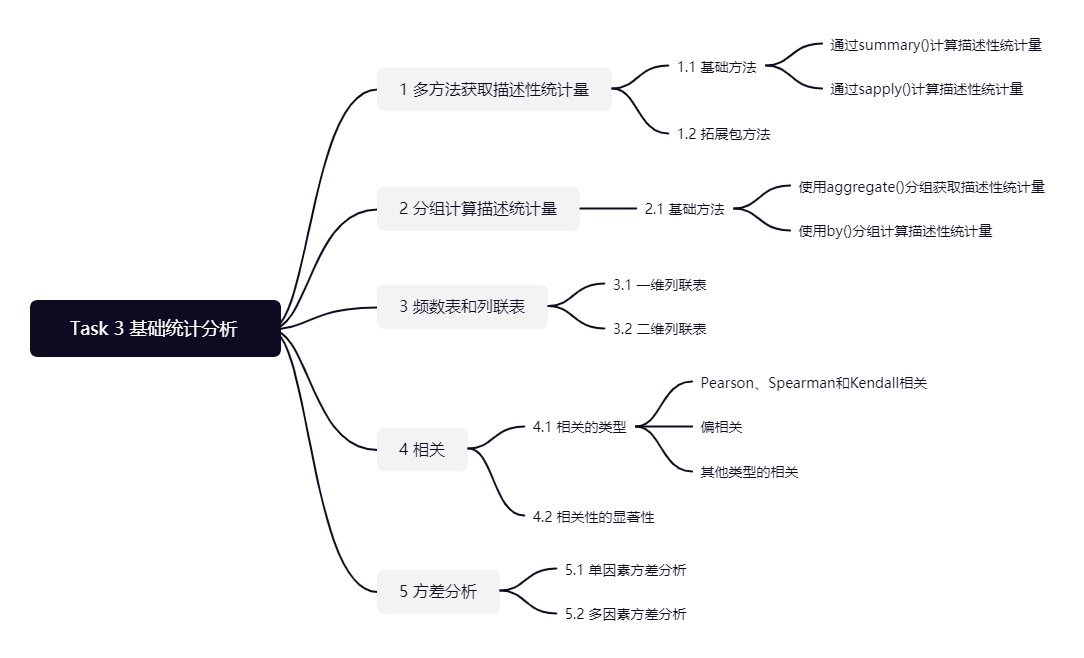
\includegraphics[width=1\textwidth,height=\textheight]{./image/task03_structure.png}

\hypertarget{ux51c6ux5907ux5de5ux4f5c-1}{%
\subsection*{准备工作}\label{ux51c6ux5907ux5de5ux4f5c-1}}


如果没有相关的包,则使用\passthrough{\lstinline!install.packages('package\_name')!}进行安装以下包。

\begin{lstlisting}[language=R]
library(pastecs)
library(psych)
library(ggm)
\end{lstlisting}

读取数据,使用H1N1流感数据集和波士顿房价数据集。

\begin{lstlisting}[language=R]
flu <- read.table("./datasets/h1n1_flu.csv", header = TRUE, sep = ",")
housing <- read.csv("./datasets/BostonHousing.csv", header = TRUE)
\end{lstlisting}

\hypertarget{ux591aux79cdux65b9ux6cd5ux83b7ux53d6ux63cfux8ff0ux6027ux7edfux8ba1ux91cf}{%
\subsection{多种方法获取描述性统计量}\label{ux591aux79cdux65b9ux6cd5ux83b7ux53d6ux63cfux8ff0ux6027ux7edfux8ba1ux91cf}}

\hypertarget{ux57faux7840ux65b9ux6cd5}{%
\subsubsection{基础方法}\label{ux57faux7840ux65b9ux6cd5}}

通过summary计算数值型变量的最大值、最小值、分位数以及均值,类别变量计算频数统计。

\begin{lstlisting}[language=R]
summary(flu[c("household_children", "sex")])
\end{lstlisting}

\begin{lstlisting}
##  household_children     sex           
##  Min.   :0.0000     Length:26707      
##  1st Qu.:0.0000     Class :character  
##  Median :0.0000     Mode  :character  
##  Mean   :0.5346                       
##  3rd Qu.:1.0000                       
##  Max.   :3.0000                       
##  NA's   :249
\end{lstlisting}

\begin{lstlisting}[language=R]
summary(flu[c("h1n1_concern", "h1n1_knowledge")])
\end{lstlisting}

\begin{lstlisting}
##   h1n1_concern   h1n1_knowledge 
##  Min.   :0.000   Min.   :0.000  
##  1st Qu.:1.000   1st Qu.:1.000  
##  Median :2.000   Median :1.000  
##  Mean   :1.618   Mean   :1.263  
##  3rd Qu.:2.000   3rd Qu.:2.000  
##  Max.   :3.000   Max.   :2.000  
##  NA's   :92      NA's   :116
\end{lstlisting}

通过 sapply() 计算描述性统计量,先定义统计函数,在进行聚合计算。

\begin{lstlisting}[language=R]
mystats <- function(x, na.omit = FALSE) {
  if (na.omit) {
    x <- x[!is.na(x)]
  }
  m <- mean(x)
  n <- length(x)
  s <- sd(x)
  skew <- sum((x - m)^3 / s^3) / n
  kurt <- sum((x - m)^4 / s^4) / n - 3
  return(c(n = n, mean = m, stdev = s, skew = skew, kurtosis = kurt))
}

sapply(flu[c("h1n1_concern", "h1n1_knowledge")], mystats)
\end{lstlisting}

\begin{lstlisting}
##          h1n1_concern h1n1_knowledge
## n               26707          26707
## mean               NA             NA
## stdev              NA             NA
## skew               NA             NA
## kurtosis           NA             NA
\end{lstlisting}

\hypertarget{ux62d3ux5c55ux5305ux65b9ux6cd5}{%
\subsubsection{拓展包方法}\label{ux62d3ux5c55ux5305ux65b9ux6cd5}}

通过pastecs包中的 stat.desc()函数计算描述性统计量,可以得到中位数、平均数、平均数的标准误、平均数置信度为95\%的置信区间、方差、标准差以及变异系数。

\begin{lstlisting}[language=R]
stat.desc(flu[c("household_children", "sex")])
\end{lstlisting}

\begin{lstlisting}
##              household_children sex
## nbr.val            2.645800e+04  NA
## nbr.null           1.867200e+04  NA
## nbr.na             2.490000e+02  NA
## min                0.000000e+00  NA
## max                3.000000e+00  NA
## range              3.000000e+00  NA
## sum                1.414400e+04  NA
## median             0.000000e+00  NA
## mean               5.345831e-01  NA
## SE.mean            5.706247e-03  NA
## CI.mean.0.95       1.118455e-02  NA
## var                8.615057e-01  NA
## std.dev            9.281733e-01  NA
## coef.var           1.736256e+00  NA
\end{lstlisting}

通过psych包中的describe()计算描述性统计量。

\begin{lstlisting}[language=R]
describe(flu[c("household_children", "sex")])
\end{lstlisting}

\begin{lstlisting}
##                    vars     n mean   sd median trimmed mad min max range skew
## household_children    1 26458 0.53 0.93      0    0.34   0   0   3     3 1.54
## sex*                  2 26707 1.41 0.49      1    1.38   0   1   2     1 0.38
##                    kurtosis   se
## household_children     1.04 0.01
## sex*                  -1.85 0.00
\end{lstlisting}

\hypertarget{ux5206ux7ec4ux8ba1ux7b97ux63cfux8ff0ux6027ux7edfux8ba1}{%
\subsection{分组计算描述性统计}\label{ux5206ux7ec4ux8ba1ux7b97ux63cfux8ff0ux6027ux7edfux8ba1}}

\hypertarget{ux57faux7840ux65b9ux6cd5-1}{%
\subsubsection{基础方法}\label{ux57faux7840ux65b9ux6cd5-1}}

\hypertarget{ux4f7fux7528aggregateux5206ux7ec4ux83b7ux53d6ux63cfux8ff0ux6027ux7edfux8ba1}{%
\paragraph*{使用aggregate()分组获取描述性统计}\label{ux4f7fux7528aggregateux5206ux7ec4ux83b7ux53d6ux63cfux8ff0ux6027ux7edfux8ba1}}
\addcontentsline{toc}{paragraph}{使用aggregate()分组获取描述性统计}

\begin{enumerate}
\def\labelenumi{\arabic{enumi}.}
\tightlist
\item
  分组计算不同性别收入贫困计数。
\item
  是否属于查尔斯河的房价中位数平均值。
\end{enumerate}

\begin{lstlisting}[language=R]
aggregate(flu[c("income_poverty")], by = list(sex = flu$sex), length)
\end{lstlisting}

\begin{lstlisting}
##      sex income_poverty
## 1 Female          15858
## 2   Male          10849
\end{lstlisting}

\begin{lstlisting}[language=R]
aggregate(housing$medv, by = list(medv = housing$chas), FUN = mean)
\end{lstlisting}

\begin{lstlisting}
##   medv        x
## 1    0 22.09384
## 2    1 28.44000
\end{lstlisting}

\hypertarget{ux4f7fux7528-by-ux5206ux7ec4ux8ba1ux7b97ux63cfux8ff0ux6027ux7edfux8ba1ux91cf}{%
\paragraph*{使用 by() 分组计算描述性统计量}\label{ux4f7fux7528-by-ux5206ux7ec4ux8ba1ux7b97ux63cfux8ff0ux6027ux7edfux8ba1ux91cf}}
\addcontentsline{toc}{paragraph}{使用 by() 分组计算描述性统计量}

\begin{lstlisting}[language=R]
by(flu[c("income_poverty", "sex")], flu$sex, length)
\end{lstlisting}

\begin{lstlisting}
## flu$sex: Female
## [1] 2
## ------------------------------------------------------------ 
## flu$sex: Male
## [1] 2
\end{lstlisting}

\hypertarget{ux9891ux6570ux8868ux548cux5217ux8054ux8868}{%
\subsection{频数表和列联表}\label{ux9891ux6570ux8868ux548cux5217ux8054ux8868}}

\begin{lstlisting}[language=R]
table(flu$sex)
\end{lstlisting}

\begin{lstlisting}
## 
## Female   Male 
##  15858  10849
\end{lstlisting}

\hypertarget{ux76f8ux5173}{%
\subsection{相关}\label{ux76f8ux5173}}

\hypertarget{ux76f8ux5173ux7684ux7c7bux578b}{%
\subsubsection{相关的类型}\label{ux76f8ux5173ux7684ux7c7bux578b}}

\hypertarget{pearsonspearmanux548ckendallux76f8ux5173}{%
\paragraph*{Pearson、Spearman和Kendall相关}\label{pearsonspearmanux548ckendallux76f8ux5173}}
\addcontentsline{toc}{paragraph}{Pearson、Spearman和Kendall相关}

R可以计算多种相关系数,包括Pearson相关系数、Spearman相关系数、Kendall相关系数、偏相关系数、多分格(polychoric)相关系数和多系列(polyserial)相关系数。
1. 计算房价数据的相关系数,默认是Pearson相关系数。

\begin{lstlisting}[language=R]
cor(housing)
\end{lstlisting}

\begin{lstlisting}
##                    X        crim          zn       indus         chas
## X        1.000000000  0.40740717 -0.10339336  0.39943885 -0.003759115
## crim     0.407407172  1.00000000 -0.20046922  0.40658341 -0.055891582
## zn      -0.103393357 -0.20046922  1.00000000 -0.53382819 -0.042696719
## indus    0.399438850  0.40658341 -0.53382819  1.00000000  0.062938027
## chas    -0.003759115 -0.05589158 -0.04269672  0.06293803  1.000000000
## nox      0.398736174  0.42097171 -0.51660371  0.76365145  0.091202807
## rm      -0.079971150 -0.21924670  0.31199059 -0.39167585  0.091251225
## age      0.203783510  0.35273425 -0.56953734  0.64477851  0.086517774
## dis     -0.302210959 -0.37967009  0.66440822 -0.70802699 -0.099175780
## rad      0.686001976  0.62550515 -0.31194783  0.59512927 -0.007368241
## tax      0.666625924  0.58276431 -0.31456332  0.72076018 -0.035586518
## ptratio  0.291074227  0.28994558 -0.39167855  0.38324756 -0.121515174
## b       -0.295041232 -0.38506394  0.17552032 -0.35697654  0.048788485
## lstat    0.258464770  0.45562148 -0.41299457  0.60379972 -0.053929298
## medv    -0.226603643 -0.38830461  0.36044534 -0.48372516  0.175260177
##                 nox          rm         age         dis          rad
## X        0.39873617 -0.07997115  0.20378351 -0.30221096  0.686001976
## crim     0.42097171 -0.21924670  0.35273425 -0.37967009  0.625505145
## zn      -0.51660371  0.31199059 -0.56953734  0.66440822 -0.311947826
## indus    0.76365145 -0.39167585  0.64477851 -0.70802699  0.595129275
## chas     0.09120281  0.09125123  0.08651777 -0.09917578 -0.007368241
## nox      1.00000000 -0.30218819  0.73147010 -0.76923011  0.611440563
## rm      -0.30218819  1.00000000 -0.24026493  0.20524621 -0.209846668
## age      0.73147010 -0.24026493  1.00000000 -0.74788054  0.456022452
## dis     -0.76923011  0.20524621 -0.74788054  1.00000000 -0.494587930
## rad      0.61144056 -0.20984667  0.45602245 -0.49458793  1.000000000
## tax      0.66802320 -0.29204783  0.50645559 -0.53443158  0.910228189
## ptratio  0.18893268 -0.35550149  0.26151501 -0.23247054  0.464741179
## b       -0.38005064  0.12806864 -0.27353398  0.29151167 -0.444412816
## lstat    0.59087892 -0.61380827  0.60233853 -0.49699583  0.488676335
## medv    -0.42732077  0.69535995 -0.37695457  0.24992873 -0.381626231
##                 tax    ptratio           b      lstat       medv
## X        0.66662592  0.2910742 -0.29504123  0.2584648 -0.2266036
## crim     0.58276431  0.2899456 -0.38506394  0.4556215 -0.3883046
## zn      -0.31456332 -0.3916785  0.17552032 -0.4129946  0.3604453
## indus    0.72076018  0.3832476 -0.35697654  0.6037997 -0.4837252
## chas    -0.03558652 -0.1215152  0.04878848 -0.0539293  0.1752602
## nox      0.66802320  0.1889327 -0.38005064  0.5908789 -0.4273208
## rm      -0.29204783 -0.3555015  0.12806864 -0.6138083  0.6953599
## age      0.50645559  0.2615150 -0.27353398  0.6023385 -0.3769546
## dis     -0.53443158 -0.2324705  0.29151167 -0.4969958  0.2499287
## rad      0.91022819  0.4647412 -0.44441282  0.4886763 -0.3816262
## tax      1.00000000  0.4608530 -0.44180801  0.5439934 -0.4685359
## ptratio  0.46085304  1.0000000 -0.17738330  0.3740443 -0.5077867
## b       -0.44180801 -0.1773833  1.00000000 -0.3660869  0.3334608
## lstat    0.54399341  0.3740443 -0.36608690  1.0000000 -0.7376627
## medv    -0.46853593 -0.5077867  0.33346082 -0.7376627  1.0000000
\end{lstlisting}

\begin{enumerate}
\def\labelenumi{\arabic{enumi}.}
\setcounter{enumi}{1}
\tightlist
\item
  指定计算Spearman相关系数
\end{enumerate}

\begin{lstlisting}[language=R]
cor(housing, method = "spearman")
\end{lstlisting}

\begin{lstlisting}
##                    X        crim         zn       indus         chas
## X        1.000000000  0.46103705 -0.1605047  0.32462127 -0.003759115
## crim     0.461037054  1.00000000 -0.5716602  0.73552374  0.041536888
## zn      -0.160504702 -0.57166021  1.0000000 -0.64281060 -0.041936998
## indus    0.324621271  0.73552374 -0.6428106  1.00000000  0.089841379
## chas    -0.003759115  0.04153689 -0.0419370  0.08984138  1.000000000
## nox      0.432491886  0.82146466 -0.6348284  0.79118913  0.068426283
## rm      -0.035641354 -0.30911647  0.3610737 -0.41530129  0.058812916
## age      0.208323439  0.70413998 -0.5444226  0.67948671  0.067791779
## dis     -0.373498683 -0.74498614  0.6146265 -0.75707970 -0.080248080
## rad      0.588480705  0.72780697 -0.2787672  0.45550745  0.024578885
## tax      0.536928176  0.72904490 -0.3713945  0.66436139 -0.044485772
## ptratio  0.297897432  0.46528319 -0.4484754  0.43371046 -0.136064621
## b       -0.154474321 -0.36055532  0.1631351 -0.28583984 -0.039810497
## lstat    0.257542491  0.63476026 -0.4900739  0.63874741 -0.050574829
## medv    -0.273633481 -0.55889095  0.4381790 -0.57825539  0.140612154
##                 nox          rm         age         dis         rad         tax
## X        0.43249189 -0.03564135  0.20832344 -0.37349868  0.58848071  0.53692818
## crim     0.82146466 -0.30911647  0.70413998 -0.74498614  0.72780697  0.72904490
## zn      -0.63482840  0.36107373 -0.54442256  0.61462654 -0.27876717 -0.37139450
## indus    0.79118913 -0.41530129  0.67948671 -0.75707970  0.45550745  0.66436139
## chas     0.06842628  0.05881292  0.06779178 -0.08024808  0.02457888 -0.04448577
## nox      1.00000000 -0.31034391  0.79515291 -0.88001486  0.58642870  0.64952656
## rm      -0.31034391  1.00000000 -0.27808202  0.26316822 -0.10749220 -0.27189846
## age      0.79515291 -0.27808202  1.00000000 -0.80160979  0.41798261  0.52636644
## dis     -0.88001486  0.26316822 -0.80160979  1.00000000 -0.49580647 -0.57433641
## rad      0.58642870 -0.10749220  0.41798261 -0.49580647  1.00000000  0.70487572
## tax      0.64952656 -0.27189846  0.52636644 -0.57433641  0.70487572  1.00000000
## ptratio  0.39130908 -0.31292257  0.35538428 -0.32204056  0.31832966  0.45334546
## b       -0.29666158  0.05366004 -0.22802200  0.24959532 -0.28253261 -0.32984308
## lstat    0.63682829 -0.64083156  0.65707079 -0.56426219  0.39432245  0.53442319
## medv    -0.56260883  0.63357643 -0.54756169  0.44585685 -0.34677626 -0.56241063
##             ptratio           b       lstat       medv
## X        0.29789743 -0.15447432  0.25754249 -0.2736335
## crim     0.46528319 -0.36055532  0.63476026 -0.5588909
## zn      -0.44847543  0.16313510 -0.49007389  0.4381790
## indus    0.43371046 -0.28583984  0.63874741 -0.5782554
## chas    -0.13606462 -0.03981050 -0.05057483  0.1406122
## nox      0.39130908 -0.29666158  0.63682829 -0.5626088
## rm      -0.31292257  0.05366004 -0.64083156  0.6335764
## age      0.35538428 -0.22802200  0.65707079 -0.5475617
## dis     -0.32204056  0.24959532 -0.56426219  0.4458569
## rad      0.31832966 -0.28253261  0.39432245 -0.3467763
## tax      0.45334546 -0.32984308  0.53442319 -0.5624106
## ptratio  1.00000000 -0.07202734  0.46725885 -0.5559047
## b       -0.07202734  1.00000000 -0.21056185  0.1856641
## lstat    0.46725885 -0.21056185  1.00000000 -0.8529141
## medv    -0.55590468  0.18566412 -0.85291414  1.0000000
\end{lstlisting}

\begin{enumerate}
\def\labelenumi{\arabic{enumi}.}
\setcounter{enumi}{2}
\tightlist
\item
  城镇人均犯罪率与房价的相关系数
\end{enumerate}

\begin{lstlisting}[language=R]
x <- housing
y <- housing[c("medv")]
cor(x, y)
\end{lstlisting}

\begin{lstlisting}
##               medv
## X       -0.2266036
## crim    -0.3883046
## zn       0.3604453
## indus   -0.4837252
## chas     0.1752602
## nox     -0.4273208
## rm       0.6953599
## age     -0.3769546
## dis      0.2499287
## rad     -0.3816262
## tax     -0.4685359
## ptratio -0.5077867
## b        0.3334608
## lstat   -0.7376627
## medv     1.0000000
\end{lstlisting}

\hypertarget{ux504fux76f8ux5173}{%
\paragraph*{偏相关}\label{ux504fux76f8ux5173}}
\addcontentsline{toc}{paragraph}{偏相关}

偏相关是指在控制一个或多个定量变量时,另外两个定量变量之间的相互关系。使用ggm 包中的 pcor() 函数计算偏相关系数。

\hypertarget{ux76f8ux5173ux6027ux7684ux663eux8457ux6027ux68c0ux9a8c}{%
\subsubsection{相关性的显著性检验}\label{ux76f8ux5173ux6027ux7684ux663eux8457ux6027ux68c0ux9a8c}}

\begin{lstlisting}[language=R]
cor.test(housing[, c("crim")], housing[, c("medv")])
\end{lstlisting}

\begin{lstlisting}
## 
##  Pearson's product-moment correlation
## 
## data:  housing[, c("crim")] and housing[, c("medv")]
## t = -9.4597, df = 504, p-value < 2.2e-16
## alternative hypothesis: true correlation is not equal to 0
## 95 percent confidence interval:
##  -0.4599064 -0.3116859
## sample estimates:
##        cor 
## -0.3883046
\end{lstlisting}

\hypertarget{ux65b9ux5deeux5206ux6790}{%
\subsection{方差分析}\label{ux65b9ux5deeux5206ux6790}}

方差分析(ANOVA)又称``变异数分析''或``F检验'',用于两个及两个以上样本均数差别的显著性检验。

\hypertarget{ux5355ux56e0ux7d20ux65b9ux5deeux5206ux6790}{%
\subsubsection{单因素方差分析}\label{ux5355ux56e0ux7d20ux65b9ux5deeux5206ux6790}}

从输出结果的F检验值来看,p\textless0.05比较显著,说明是否在查尔斯河对房价有影响。

\begin{lstlisting}[language=R]
fit <- aov(housing$medv ~ housing$chas)
summary(fit)
\end{lstlisting}

\begin{lstlisting}
##               Df Sum Sq Mean Sq F value   Pr(>F)    
## housing$chas   1   1312  1312.1   15.97 7.39e-05 ***
## Residuals    504  41404    82.2                     
## ---
## Signif. codes:  0 '***' 0.001 '**' 0.01 '*' 0.05 '.' 0.1 ' ' 1
\end{lstlisting}

\hypertarget{ux591aux56e0ux7d20ux65b9ux5deeux5206ux6790}{%
\subsubsection{多因素方差分析}\label{ux591aux56e0ux7d20ux65b9ux5deeux5206ux6790}}

构建多因素方差分析,查看因子对房价的影响是否显著。

\begin{lstlisting}[language=R]
fit <- aov(housing$medv ~ housing$crim * housing$b)
summary(fit)
\end{lstlisting}

\begin{lstlisting}
##                         Df Sum Sq Mean Sq F value   Pr(>F)    
## housing$crim             1   6441    6441   96.05  < 2e-16 ***
## housing$b                1   1697    1697   25.30 6.83e-07 ***
## housing$crim:housing$b   1    917     917   13.68 0.000241 ***
## Residuals              502  33662      67                     
## ---
## Signif. codes:  0 '***' 0.001 '**' 0.01 '*' 0.05 '.' 0.1 ' ' 1
\end{lstlisting}

\hypertarget{ux672cux7ae0ux4f5cux8005-3}{%
\subsection*{本章作者}\label{ux672cux7ae0ux4f5cux8005-3}}


\textbf{杨佳达}

\begin{quote}
数据挖掘师,Datawhale成员,目前在国内某第三方数据服务公司做数据分析挖掘及数据产品\\
\url{https://github.com/yangjiada}
\end{quote}

\hypertarget{ux5173ux4e8edatawhale-3}{%
\subsection*{关于Datawhale}\label{ux5173ux4e8edatawhale-3}}


Datawhale 是一个专注于数据科学与AI领域的开源组织,汇集了众多领域院校和知名企业的优秀学习者,聚合了一群有开源精神和探索精神的团队成员。Datawhale 以``for the learner,和学习者一起成长''为愿景,鼓励真实地展现自我、开放包容、互信互助、敢于试错和勇于担当。同时 Datawhale 用开源的理念去探索开源内容、开源学习和开源方案,赋能人才培养,助力人才成长,建立起人与人,人与知识,人与企业和人与未来的联结。 本次数据挖掘路径学习,专题知识将在天池分享,详情可关注 Datawhale:


\includegraphics[width=3.58in]{image/logo}

\hypertarget{task-04}{%
\section{数据可视化}\label{task-04}}

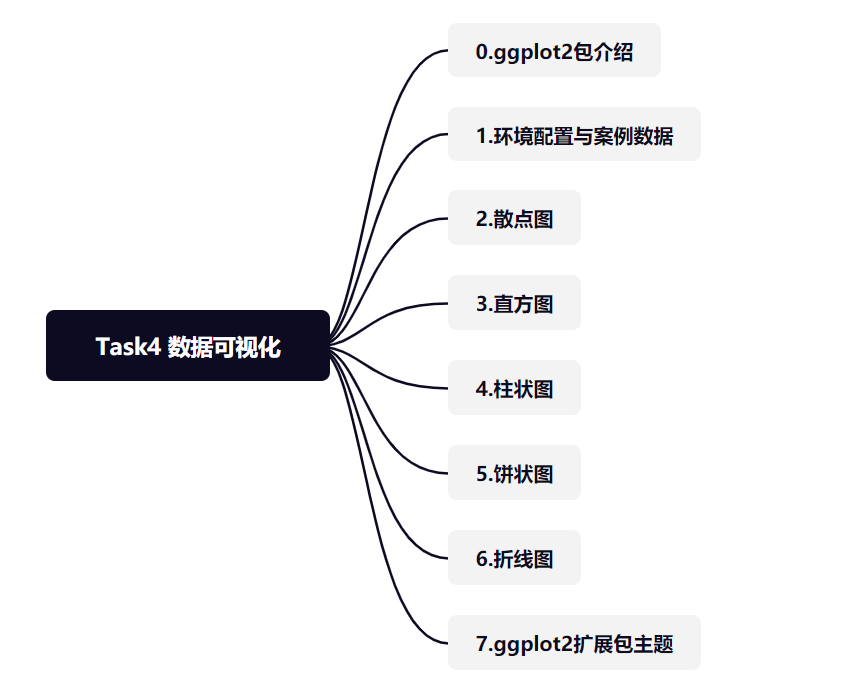
\includegraphics[width=0.6\textwidth,height=\textheight]{./image/task04_structure.png}

\hypertarget{ggplot2ux5305ux4ecbux7ecd}{%
\subsection*{ggplot2包介绍}\label{ggplot2ux5305ux4ecbux7ecd}}


ggplot2包由Hadley Wickham编写,提供了一种基于Wilkinson所述图形语法的图形系统。ggplot2包的目标是提供一个全面的、基于语法的、连贯一致的图形生成系统,允许用户创建新颖的、有创新性的数据可视化图形。

总的来说有以下几点:

\begin{itemize}
\tightlist
\item
  ggplot2的核心理念是将绘图与数据分离,数据相关的绘图与数据无关的绘图分离
\item
  ggplot2保有命令式作图的调整函数,使其更具灵活性
\item
  ggplot2将常见的统计变换融入到了绘图中。
\item
  ggplot2是按图层作图
\end{itemize}

ggplot2图像的三个基本构成:数据、图形属性映射、几何对象

按照ggplot2的绘图理念,Plot(图)= data(数据集)+ Aesthetics(美学映射)+ Geometry(几何对象)。

例如:

\begin{lstlisting}[language=R]
# ggplot(data,aes(x=x,y=y))+geom_point()
\end{lstlisting}

\begin{itemize}
\tightlist
\item
  数据:用于绘制图形的数据
\item
  映射:aes()函数是ggplot2中的映射函数, 所谓的映射即为数据集中的数据关联到相应的图形属性过程中一种对应关系, 图形的颜色,形状,分组等都可以通过通过数据集中的变量映射。
\item
  几何对象:我们在图中实际看到的图形元素,如点、线、多边形等。
\end{itemize}

ggplot2绘图代码如同数据公式一般,只需要套相应的公式即可绘制出丰富的图形,后续的讲解也会按照此方法。

ggplot2参考链接:

\begin{itemize}
\tightlist
\item
  \url{https://ggplot2.tidyverse.org/reference/}
\item
  \url{https://ggplot2-book.org/}
\end{itemize}

ggplot2的安装方法

\begin{lstlisting}[language=R]
# install.packages("ggplot2")
\end{lstlisting}

\hypertarget{ux73afux5883ux914dux7f6e-2}{%
\subsection{环境配置}\label{ux73afux5883ux914dux7f6e-2}}

\begin{lstlisting}[language=R]
library(ggplot2) # 画图工具ggplot2
library(ggpubr) # 将多个图形拼接
library(plyr) # 数据处理包
\end{lstlisting}

在本讲中会用到ggpubr中的ggrrange这个多图拼接工具,详细使用方法参见:
\url{http://www.sthda.com/english/articles/24-ggpubr-publication-ready-plots/81-ggplot2-easy-way-to-mix-multiple-graphs-on-the-same-page/}

\hypertarget{ux6848ux4f8bux6570ux636e-1}{%
\subsubsection*{案例数据}\label{ux6848ux4f8bux6570ux636e-1}}


本节内容将会使用到两个数据集

\textbf{1.1h1n1流感问卷数据集}

h1n1流感问卷数据集是关于h1n1流感问卷调查的一个数据,属于外部数据
数据集包含26,707个受访者数据,共有32个特征+1个标签(是否接种h1n1疫苗)

读取相关的数据集

\begin{lstlisting}[language=R]
h1n1_data <- read.csv("./datasets/h1n1_flu.csv", header = TRUE)
\end{lstlisting}

\textbf{1.2波士顿房价数据集}

波士顿房价数据集属于R语言自带数据集,也可以通过外部读取

读取相关的数据集

\begin{lstlisting}[language=R]
boston_data <- read.csv("./datasets/BostonHousing.csv", header = TRUE)
\end{lstlisting}

\hypertarget{ux6563ux70b9ux56fe}{%
\subsection{散点图}\label{ux6563ux70b9ux56fe}}

散点图是指在数理统计回归分析中,数据点在直角坐标系平面上的分布图,散点图表示因变量随自变量而变化的大致趋势,由此趋势可以选择合适的函数进行经验分布的拟合,进而找到变量之间的函数关系。

散点图的优势:

\begin{itemize}
\tightlist
\item
  数据用图表来展示,显然比较直观,在工作汇报等场合能起到事半功倍的效果,让听者更容易接受,理解你所处理的数据。
\item
  散点图更偏向于研究型图表,能让我们发现变量之间隐藏的关系为我们决策作出重要的引导作用。
\item
  散点图核心的价值在于发现变量之间的关系,包括线性与非线性之间的关系。
\end{itemize}

\begin{lstlisting}[language=R]
# 读取数据
boston_data <- read.csv("./datasets/BostonHousing.csv", header = TRUE)
# 绘制简单的散点图 x轴选择的是lstat ,y轴选择的是medv
ggplot(data = boston_data, aes(x = lstat, y = medv)) +
  geom_point()
\end{lstlisting}

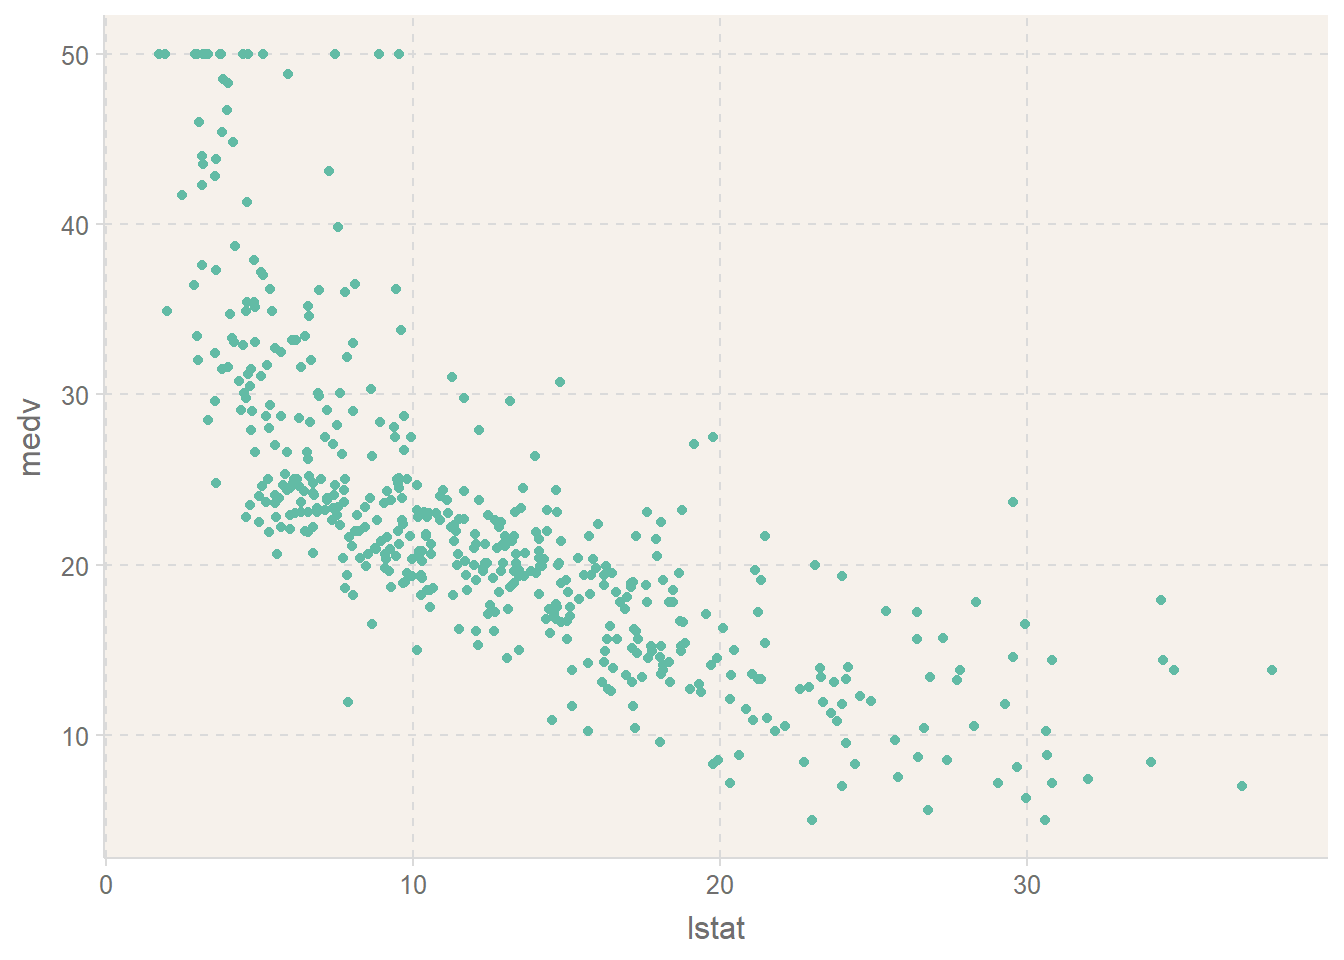
\includegraphics{RLearning_files/figure-latex/plot1-1.pdf}

上图选择的是lstat为x轴,medv为y轴绘制的散点图,x轴表示弱势群体人口所占比例,y轴表示房屋的平均价格,通过图上的数据可以看到,弱势人群的比例增加会影响房价,这2个变量呈现一定的负相关。

ggplot2可以修改散点图的性状和大小,R语言中存储了一些相关的形状
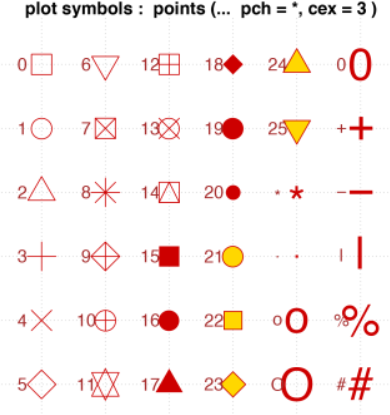
\includegraphics[width=0.5\textwidth,height=\textheight]{./image/task04_fig1.png}

size参数修改点的大小,color参数修改点的颜色

\begin{lstlisting}[language=R]
# 使用第17号形状
p1 <- ggplot(data = boston_data, aes(x = lstat, y = medv)) +
  geom_point(shape = 17)
# size参数修改点的大小,color参数修改点的颜色
p2 <- ggplot(data = boston_data, aes(x = lstat, y = medv)) +
  geom_point(size = 3, color = "red")
ggarrange(p1, p2, nrow = 1)
\end{lstlisting}

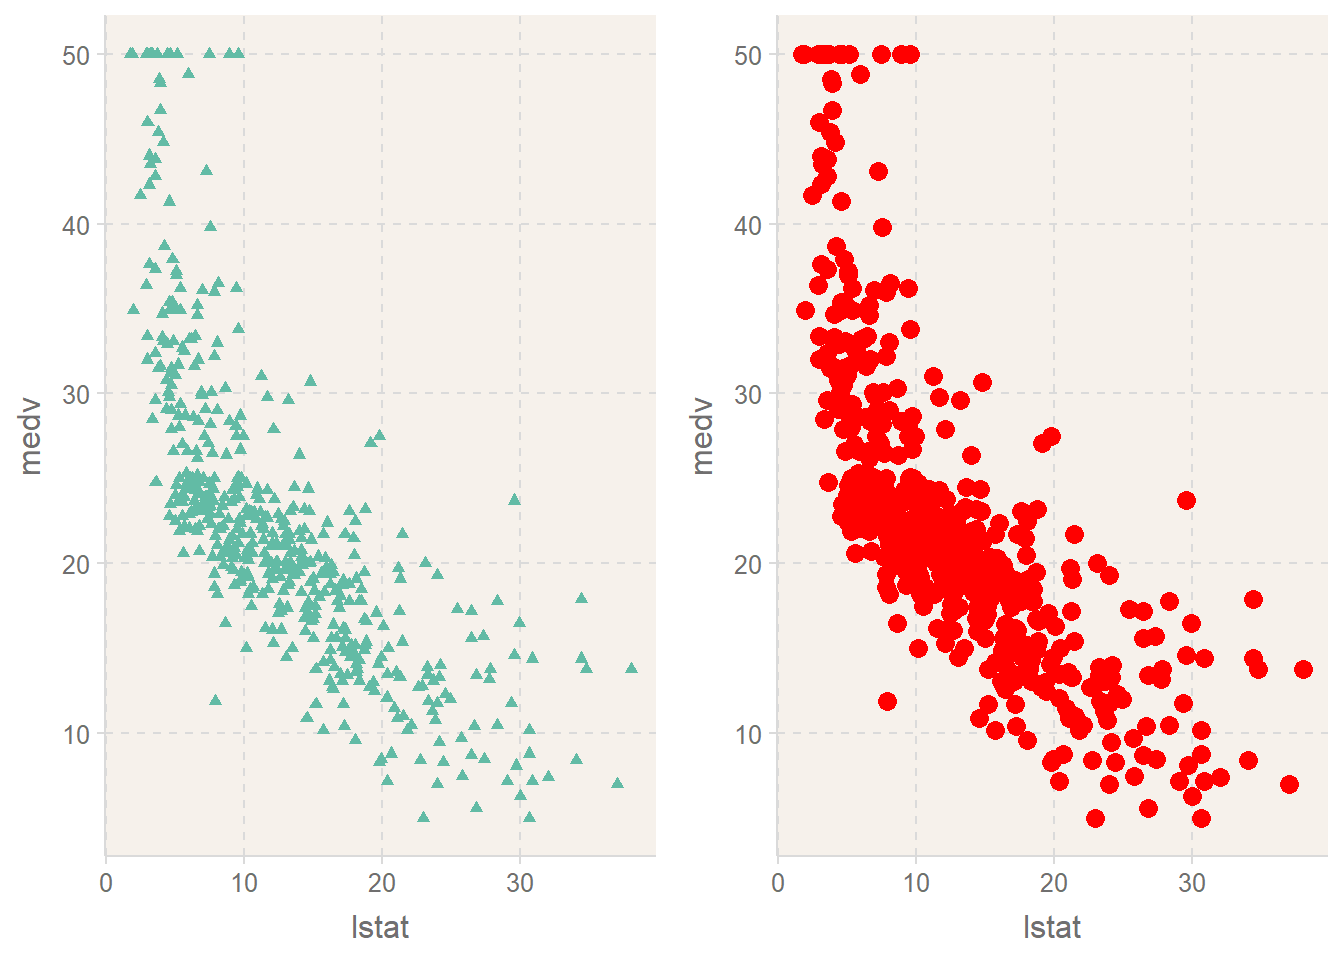
\includegraphics{RLearning_files/figure-latex/plot2-1.pdf}

可将数据集的其它属性映射到散点图的颜色属性中

\begin{lstlisting}[language=R]
p3 <- ggplot(data = boston_data, aes(x = lstat, y = medv, colour = factor(rad))) +
  geom_point()
p4 <- ggplot(data = boston_data, aes(x = lstat, y = medv, colour = rad)) +
  geom_point()
ggarrange(p3, p4, nrow = 1)
\end{lstlisting}

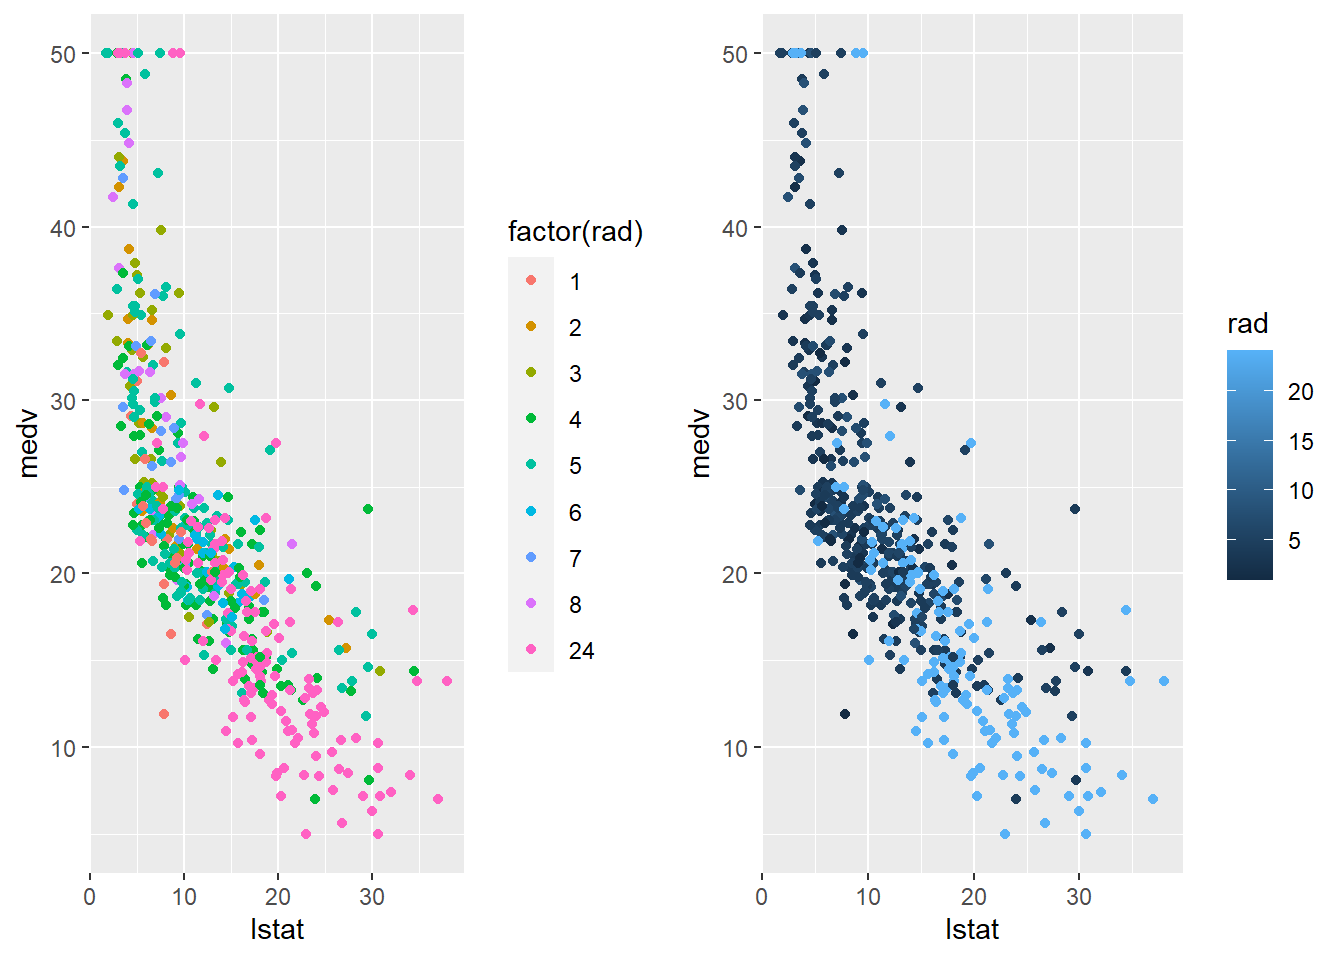
\includegraphics{RLearning_files/figure-latex/plot4-1.pdf}

ggplot2关于散点图的相关做法有很详细的介绍,相关参考链接:\url{https://ggplot2.tidyverse.org/reference/geom_point.html}

\hypertarget{ux76f4ux65b9ux56fe}{%
\subsection{直方图}\label{ux76f4ux65b9ux56fe}}

直方图是一种统计报告图,由一系列高度不等的纵向条纹或线段表示数据分布的情况。 一般用横轴表示数据类型,纵轴表示分布情况。
直方图可以很好的查看数据的分布情况,是常用的数据可视化展示图形。

我们对rad变量进行直方图分析

\begin{lstlisting}[language=R]
ggplot(data = boston_data, aes(x = rad)) +
  geom_histogram()
\end{lstlisting}

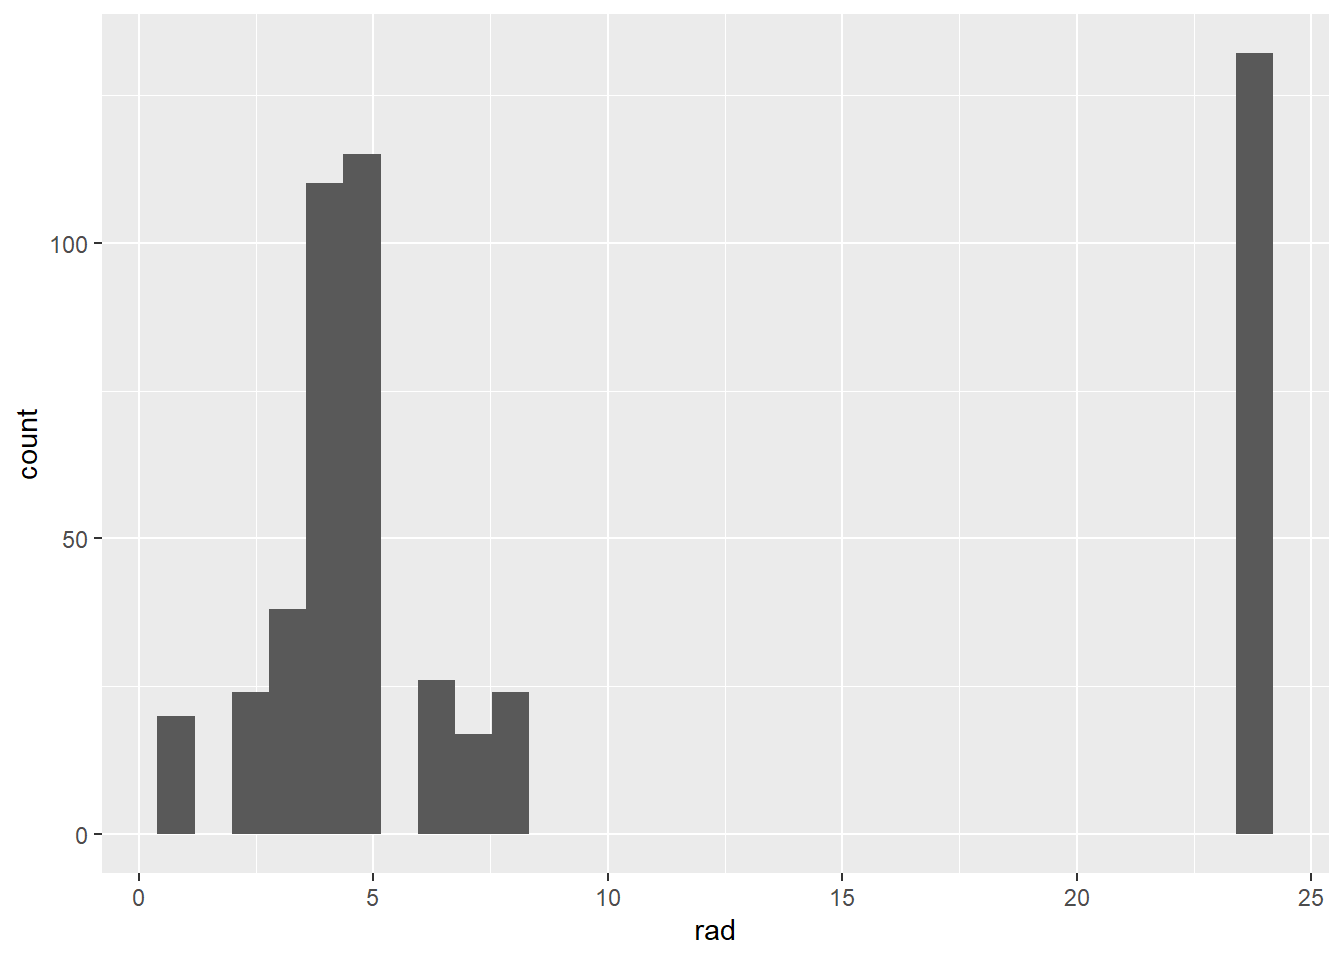
\includegraphics{RLearning_files/figure-latex/plot6-1.pdf}

可以看到ggplot2可以自动对数据进行直方图的统计

我们给直方图填充颜色,同时改变直方图类型color表示直方图的边框,fill表示直方图中的填充颜色,ggplot2支持RGB颜色表的配色方案,linetype表示直方图线的类型

RGB颜色表可以参考:\url{http://www.mgzxzs.com/sytool/se.htm}

\begin{lstlisting}[language=R]
p5 <- ggplot(data = boston_data, aes(x = rad)) +
  geom_histogram(color = "black", fill = "#69b3a2")
p6 <- ggplot(data = boston_data, aes(x = rad)) +
  geom_histogram(color = "black", fill = "#69b3a2", linetype = "dashed")
ggarrange(p5, p6, nrow = 1)
\end{lstlisting}

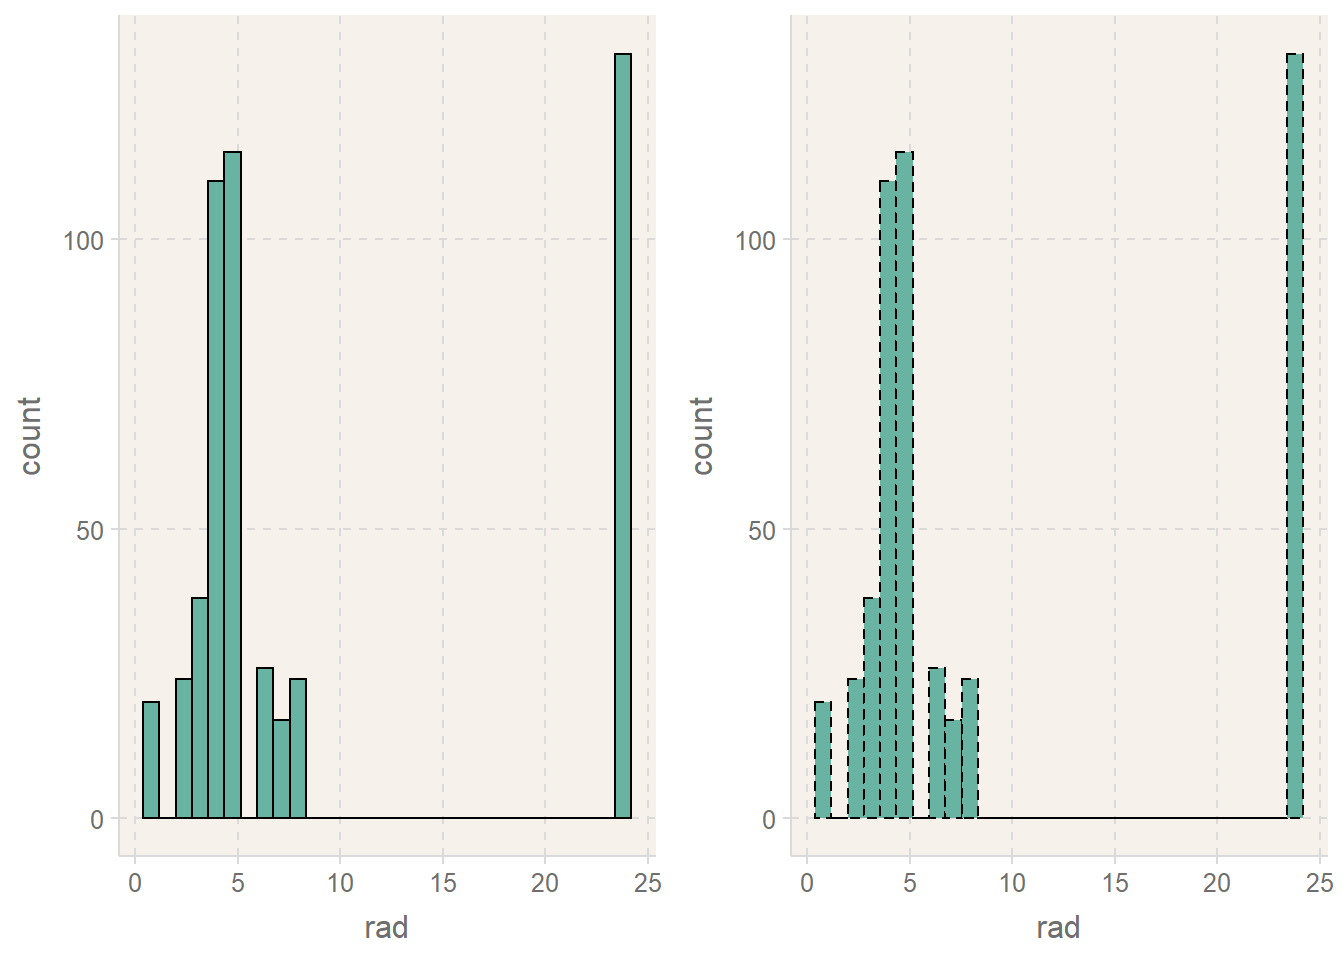
\includegraphics{RLearning_files/figure-latex/plot7-1.pdf}

ggplot2也支持在直方图上添加平均线和密度图

\begin{lstlisting}[language=R]
p7 <- p5 + geom_vline(aes(xintercept = mean(rad)), color = "blue", linetype = "dashed", size = 1)
p8 <- ggplot(data = boston_data, aes(x = rad)) +
  geom_histogram(color = "black", fill = "#69b3a2", aes(y = ..density..)) +
  geom_density(alpha = .2, fill = "#FF6666")
ggarrange(p7, p8, nrow = 1)
\end{lstlisting}

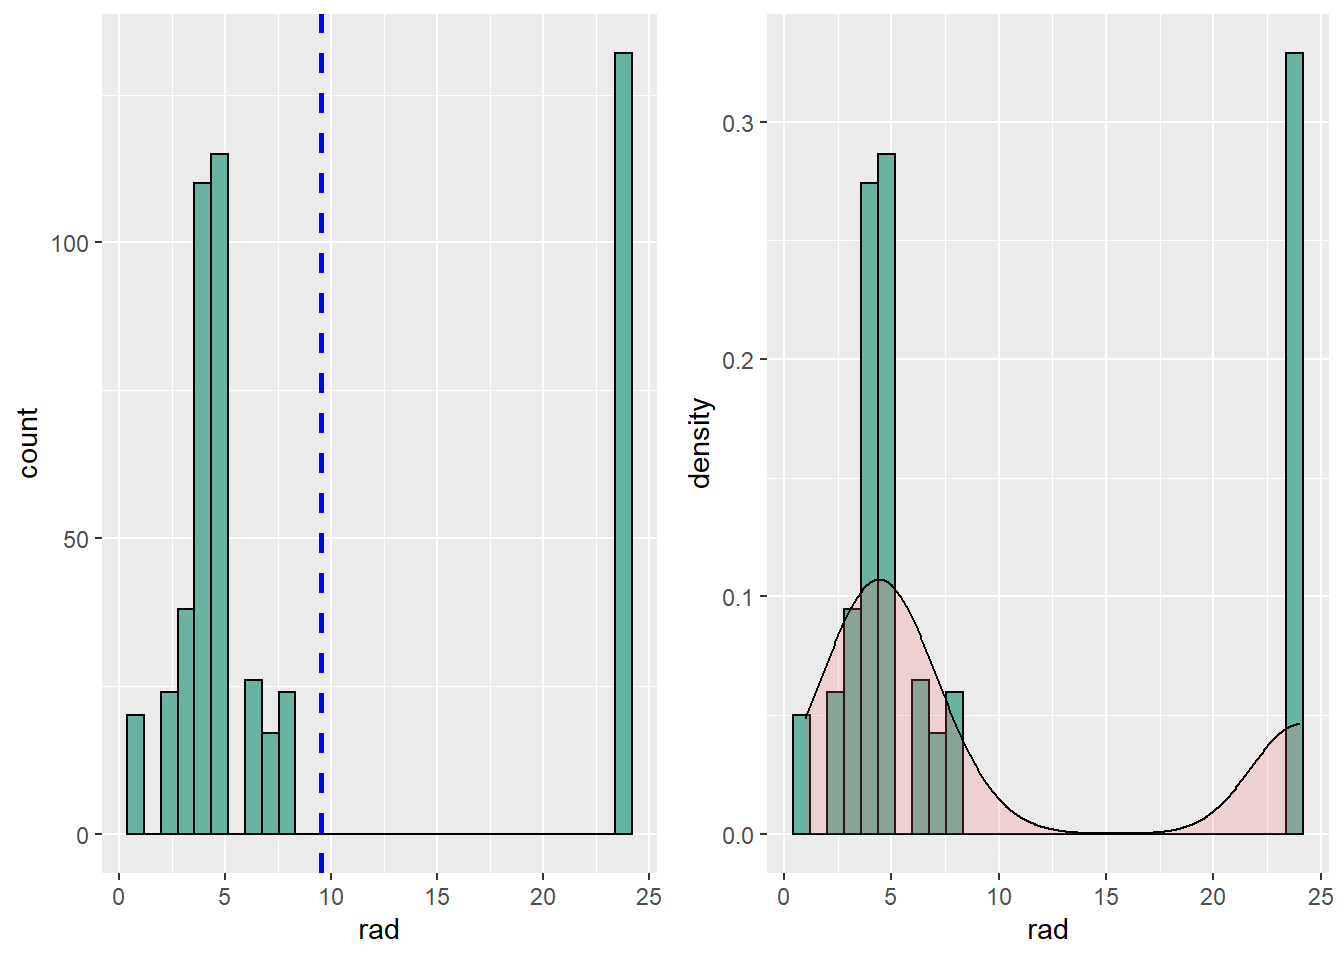
\includegraphics{RLearning_files/figure-latex/plot8-1.pdf}

ggplot2关于直方图的相关做法有很详细的介绍,相关参考链接:\url{https://ggplot2.tidyverse.org/reference/geom_histogram.html}

\hypertarget{ux67f1ux72b6ux56fe}{%
\subsection{柱状图}\label{ux67f1ux72b6ux56fe}}

柱状图是一种常用的数据可视化图形,根据翻译的不同,柱状图又叫长条图、柱状统计图、条状图、棒形图
柱状图图用来比较两个或以上的价值(不同时间或者不同条件),只有一个变量,通常利用于较小的数据集分析。长条图亦可横向排列,或用多维方式表达。需要注意的是柱状图与直方图是不同的数据可视化方法,不要弄混淆了。

对h1n1数据集中填写人的受教育情况进行可视化展示,使用pylr包中的count对edcation进行计数统计

\begin{lstlisting}[language=R]
data <- count(h1n1_data["race"])
p <- ggplot(data, aes(x = race, y = freq)) +
  geom_bar(stat = "identity")
# 也可以进行水平放置
p1 <- p + coord_flip()
ggarrange(p, p1)
\end{lstlisting}

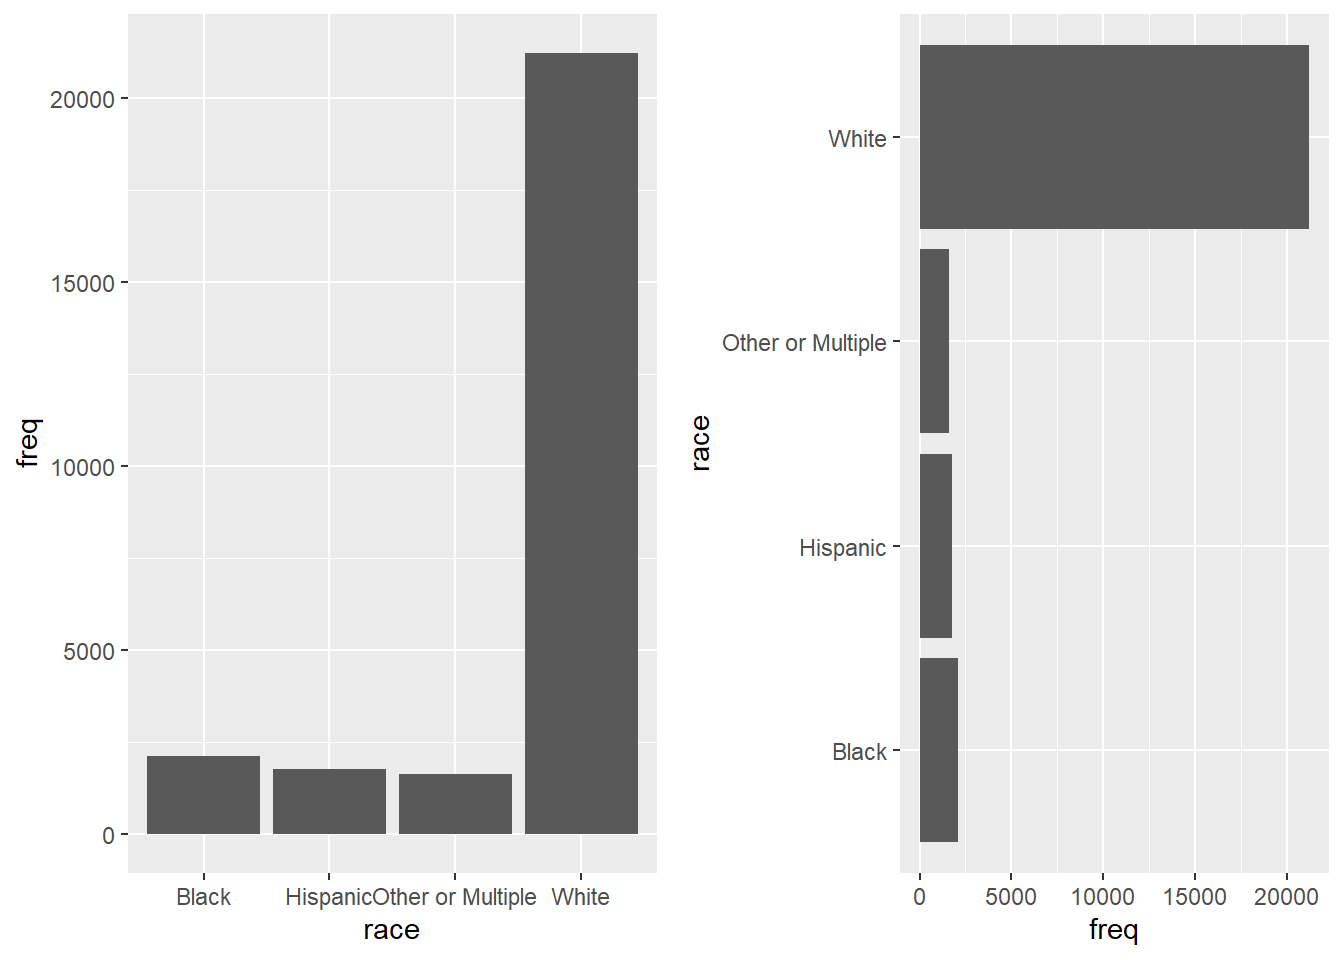
\includegraphics{RLearning_files/figure-latex/plot9-1.pdf}

可以看到左边的柱状图文字有点挡住了,我们把文字旋转45°

\begin{lstlisting}[language=R]
data <- count(h1n1_data["race"])
ggplot(data, aes(x = race, y = freq)) +
  geom_bar(stat = "identity") +
  theme(axis.text.x = element_text(angle = 45, hjust = 1))
\end{lstlisting}

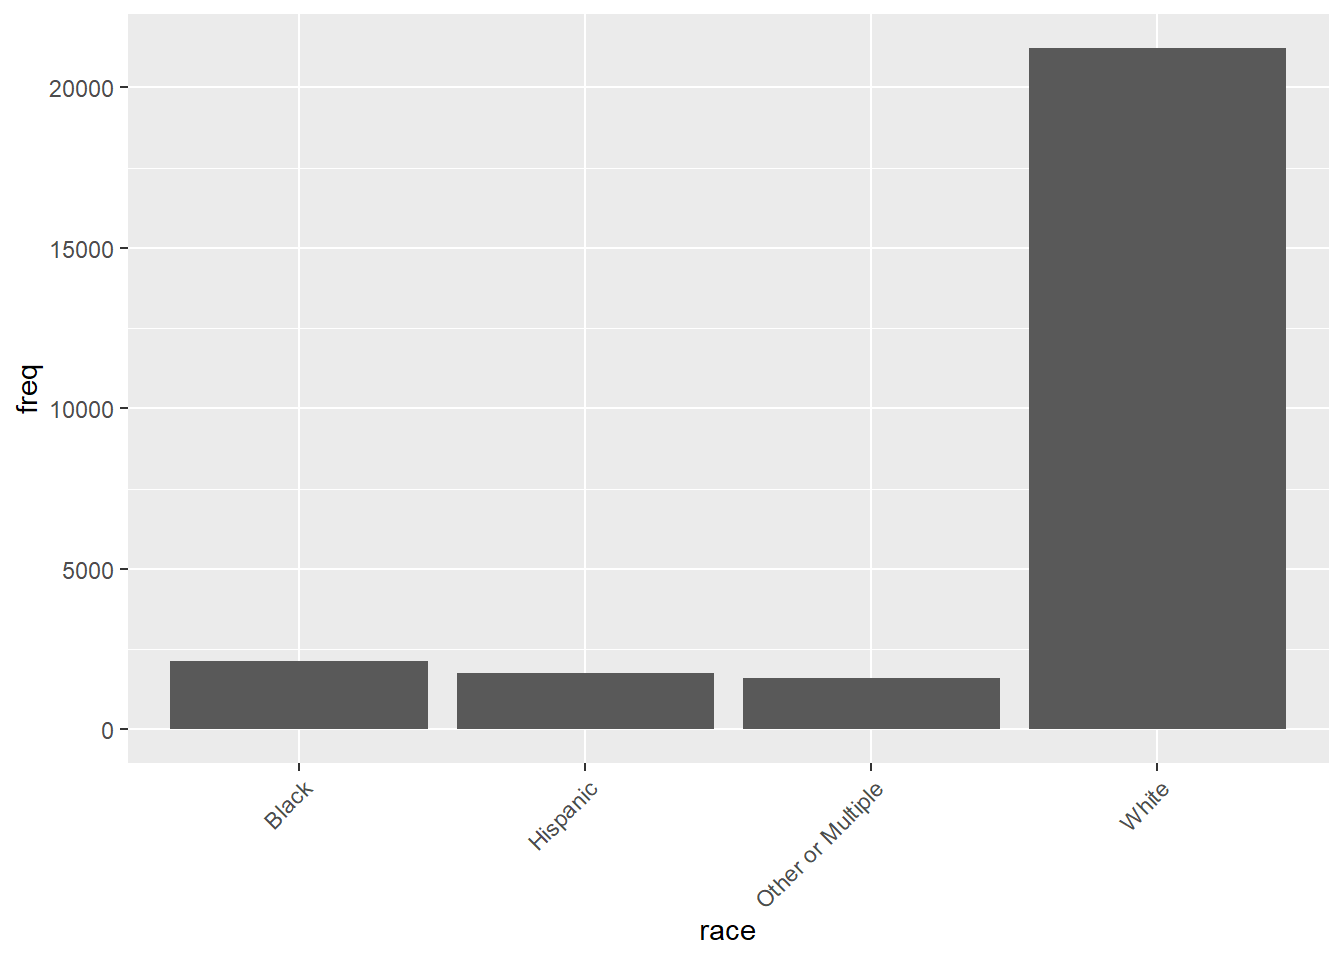
\includegraphics{RLearning_files/figure-latex/plot9a-1.pdf}

对柱状图的样式进行修改

\begin{lstlisting}[language=R]
# 更改条的宽度和颜色:
# 更改条的宽度
p2 <- ggplot(data, aes(x = race, y = freq)) +
  geom_bar(stat = "identity", width = 0.5) +
  theme(axis.text.x = element_text(angle = 45, hjust = 1))
# 改变颜色
p3 <- ggplot(data, aes(x = race, y = freq)) +
  geom_bar(stat = "identity", color = "blue", fill = "white") +
  theme(axis.text.x = element_text(angle = 45, hjust = 1))
# 最小主题+蓝色填充颜色
p4 <- ggplot(data, aes(x = race, y = freq)) +
  geom_bar(stat = "identity", fill = "steelblue") +
  theme_minimal() +
  theme(axis.text.x = element_text(angle = 45, hjust = 1))
# 选择要显示的项目
p5 <- p + scale_x_discrete(limits = c("White", "Black")) + theme(axis.text.x = element_text(angle = 45, hjust = 1))
ggarrange(p2, p3, p4, p5)
\end{lstlisting}

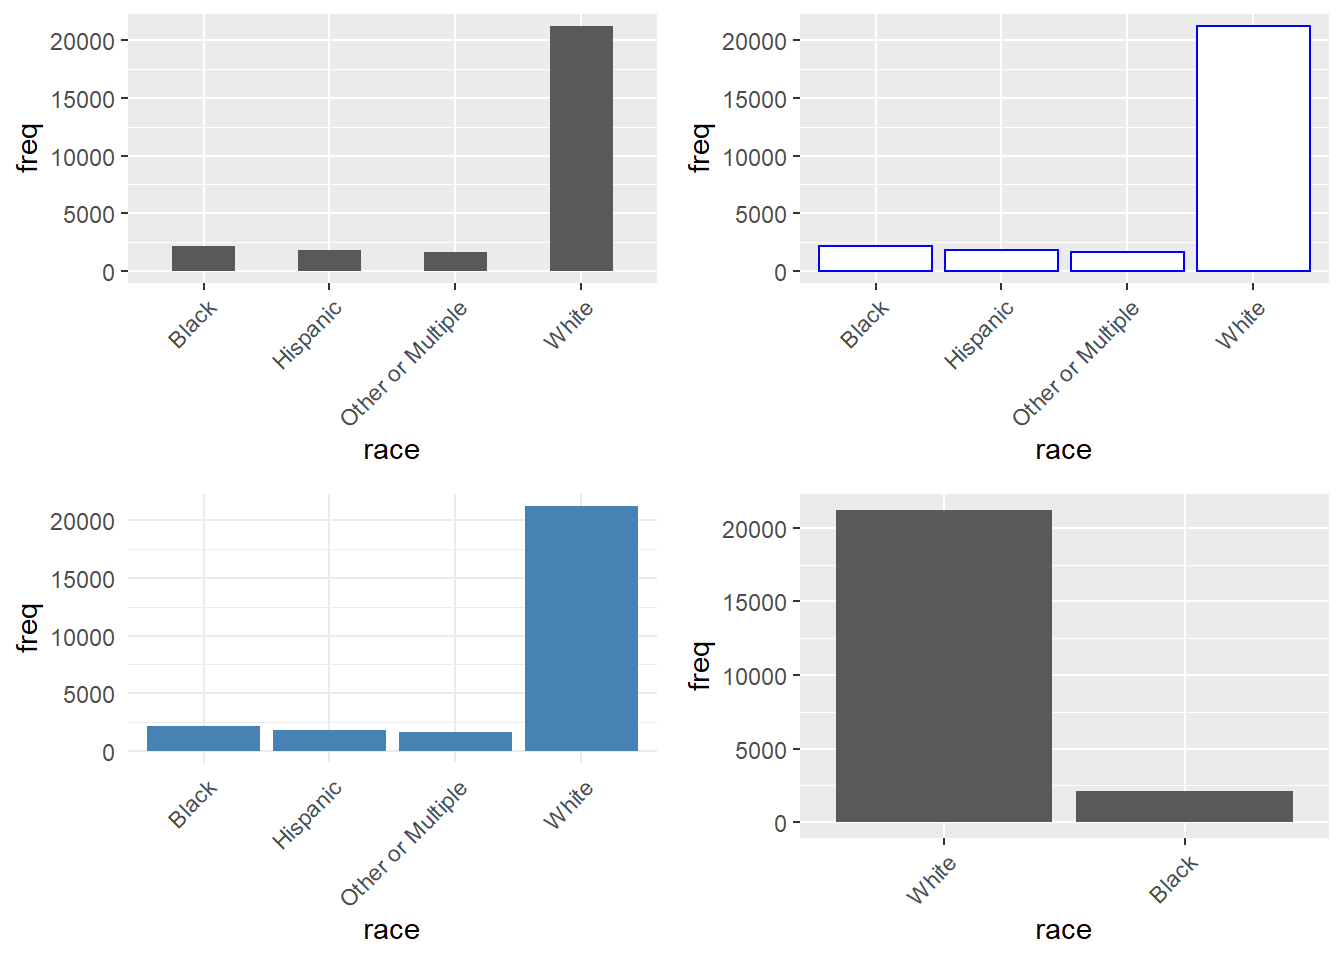
\includegraphics{RLearning_files/figure-latex/plot10-1.pdf}

对柱状图进行标签显示

\begin{lstlisting}[language=R]
p6 <- ggplot(data = data, aes(x = race, y = freq)) +
  geom_bar(stat = "identity", fill = "steelblue") +
  geom_text(aes(label = freq), vjust = -0.3, size = 3.5) +
  theme_minimal() +
  theme(axis.text.x = element_text(angle = 45, hjust = 1))
# 条形内部标签
p7 <- ggplot(data = data, aes(x = race, y = freq)) +
  geom_bar(stat = "identity", fill = "steelblue") +
  geom_text(aes(label = freq), vjust = 1.6, color = "white", size = 3.5) +
  theme_minimal() +
  theme(axis.text.x = element_text(angle = 45, hjust = 1))
ggarrange(p6, p7, nrow = 1)
\end{lstlisting}

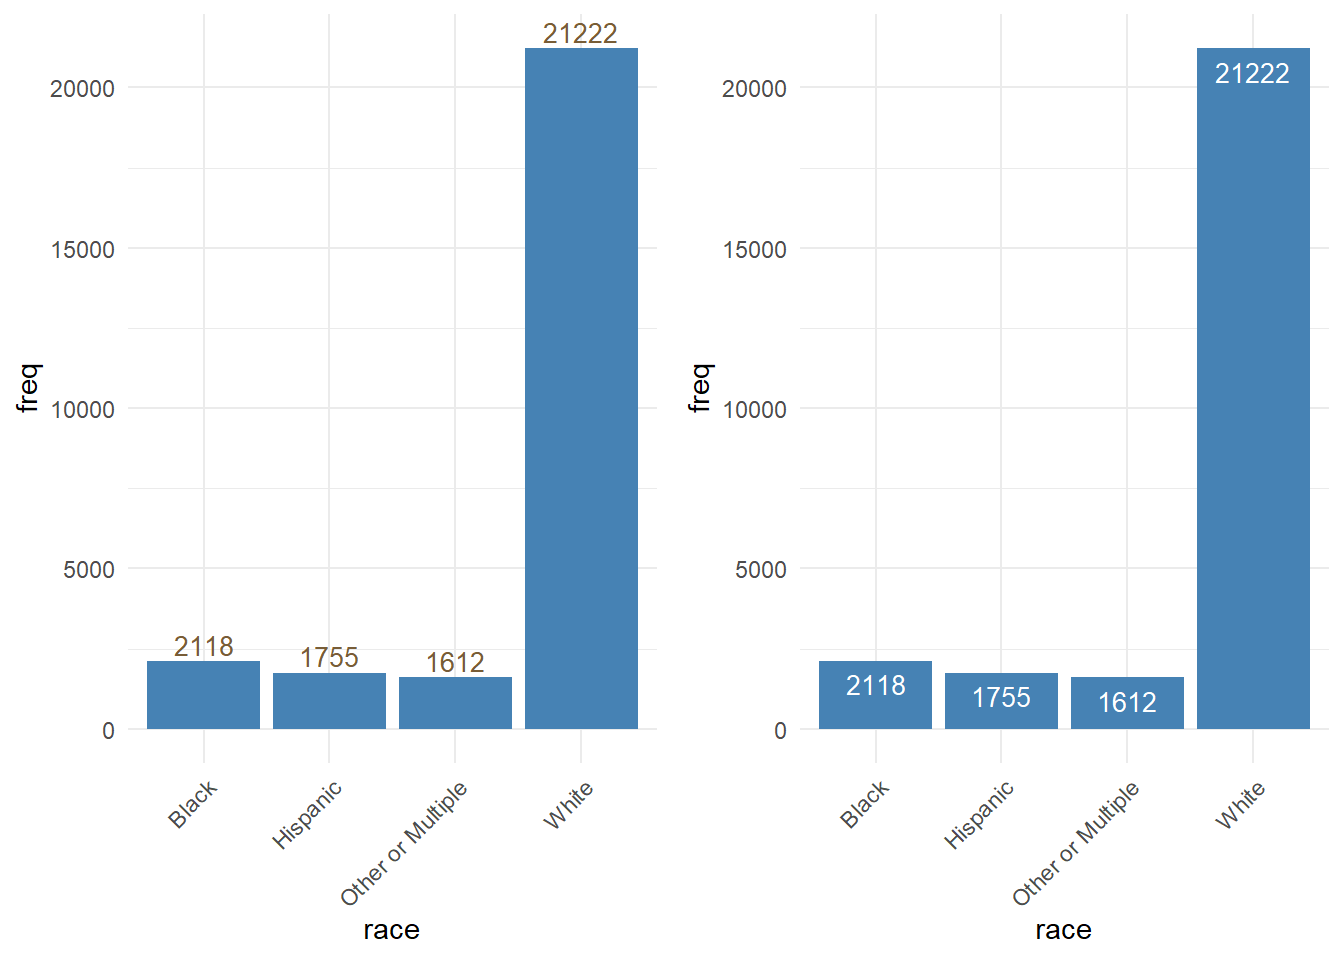
\includegraphics{RLearning_files/figure-latex/plot11-1.pdf}

如果觉得柱状图的顺序不是你想要的,可以对柱状图的顺序进行修改

\begin{lstlisting}[language=R]
data <- within(data, {
  race <- factor(race, levels = c("White", "Black", "Hispanic", "Other or Multiple"))
})
ggplot(data, aes(x = race, y = freq)) +
  geom_bar(stat = "identity", fill = "steelblue") +
  theme(axis.text.x = element_text(angle = 45, hjust = 1))
\end{lstlisting}

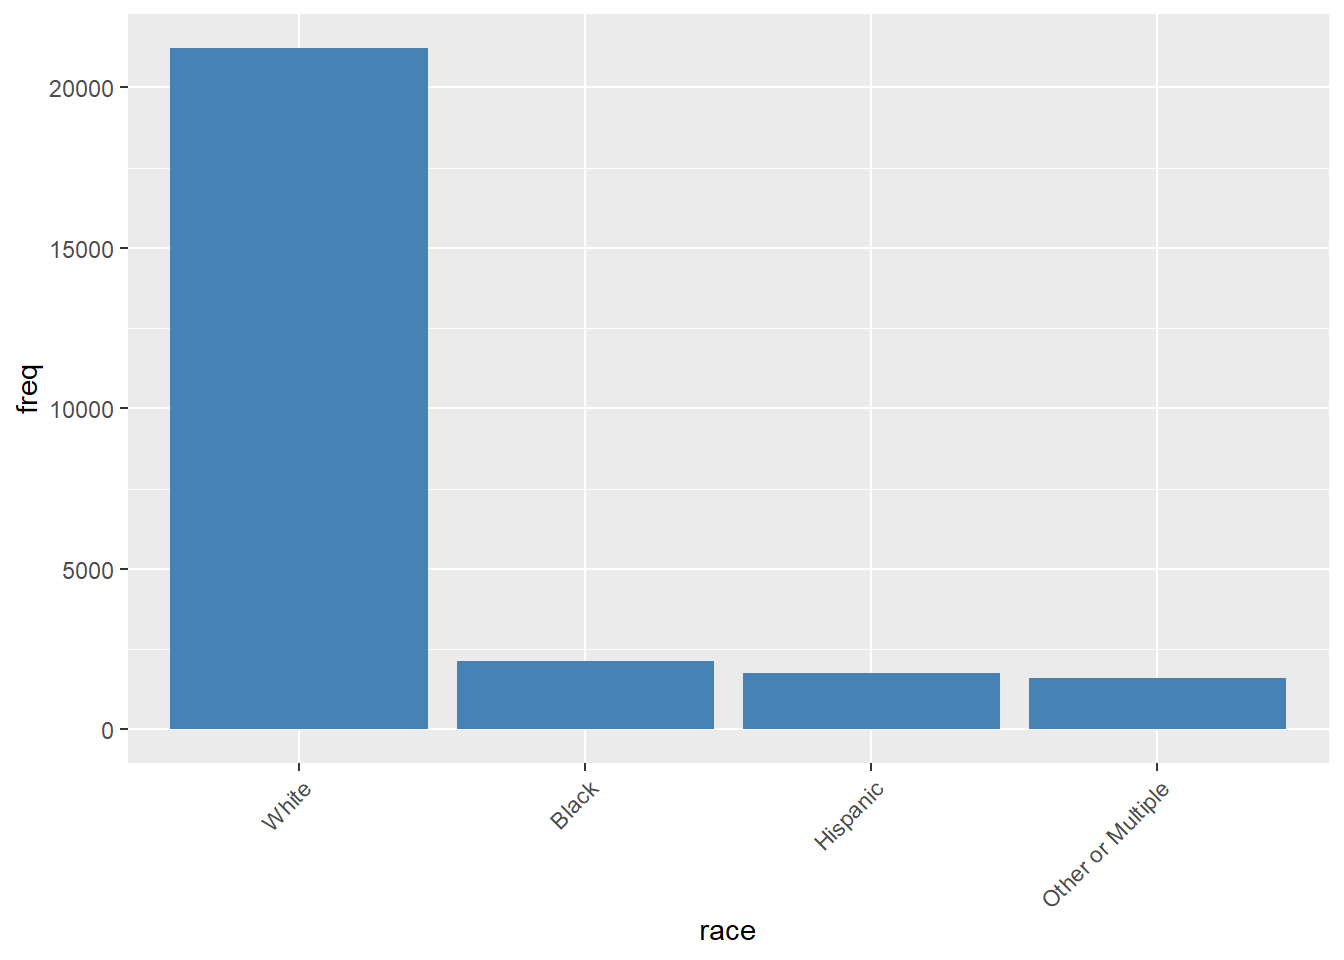
\includegraphics{RLearning_files/figure-latex/plot12-1.pdf}

ggplot2关于柱状图的相关做法有很详细的介绍,相关参考链接:
\url{https://ggplot2.tidyverse.org/reference/geom_bar.html}

\hypertarget{ux997cux72b6ux56fe}{%
\subsection{饼状图}\label{ux997cux72b6ux56fe}}

饼状图作为常用的数据可视化图形之一,广泛的使用在各个领域,能够很清楚展示数据的所占的百分比。
ggplot2并没有类似于geom\_pie()这样的函数实现饼图的绘制,但ggplot2有一个理念,就是通过极坐标变换绘制饼图

饼图在ggplot2中就是通过极坐标变换获得,在绘制饼图之前需要绘制堆叠的条形图,通过将条形图进行极坐标变换后,就能实现饼图绘制了。

对h1n1问卷表中race数据进行数据展示

\begin{lstlisting}[language=R]
data <- count(h1n1_data["race"])
ggplot(data = data, aes(x = "", y = freq, fill = race)) +
  geom_bar(stat = "identity")
\end{lstlisting}

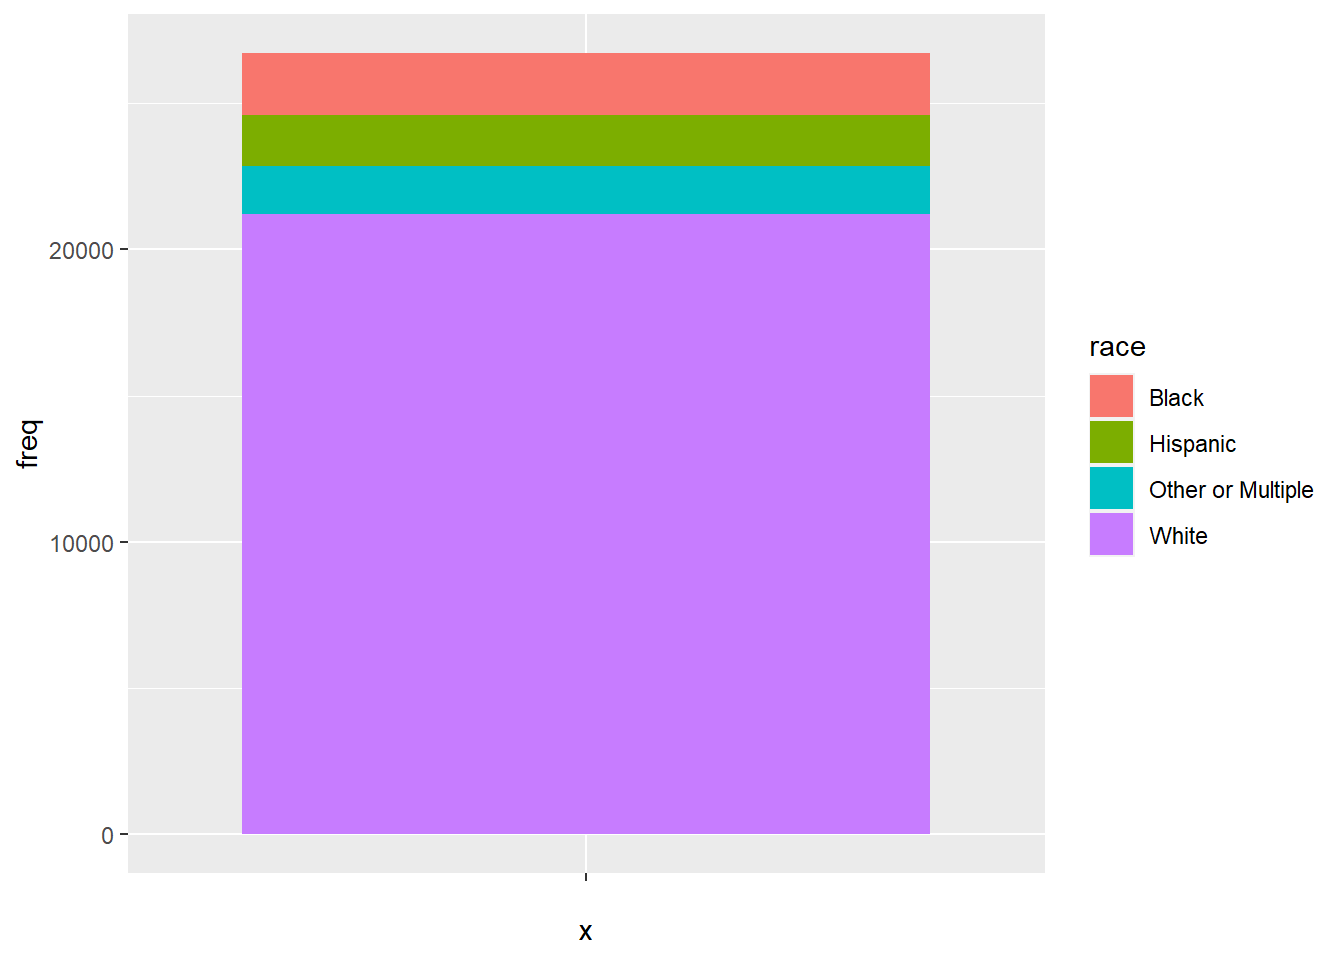
\includegraphics{RLearning_files/figure-latex/plot13-1.pdf}

堆叠的条形图绘制完后,接下来就需要进行极坐标变换了,ggplot2中coord\_polar()函数可以非常方便的实现极坐标变换。

\begin{lstlisting}[language=R]
ggplot(data = data, aes(x = "", y = freq, fill = race)) +
  geom_bar(stat = "identity") +
  coord_polar(theta = "y")
\end{lstlisting}

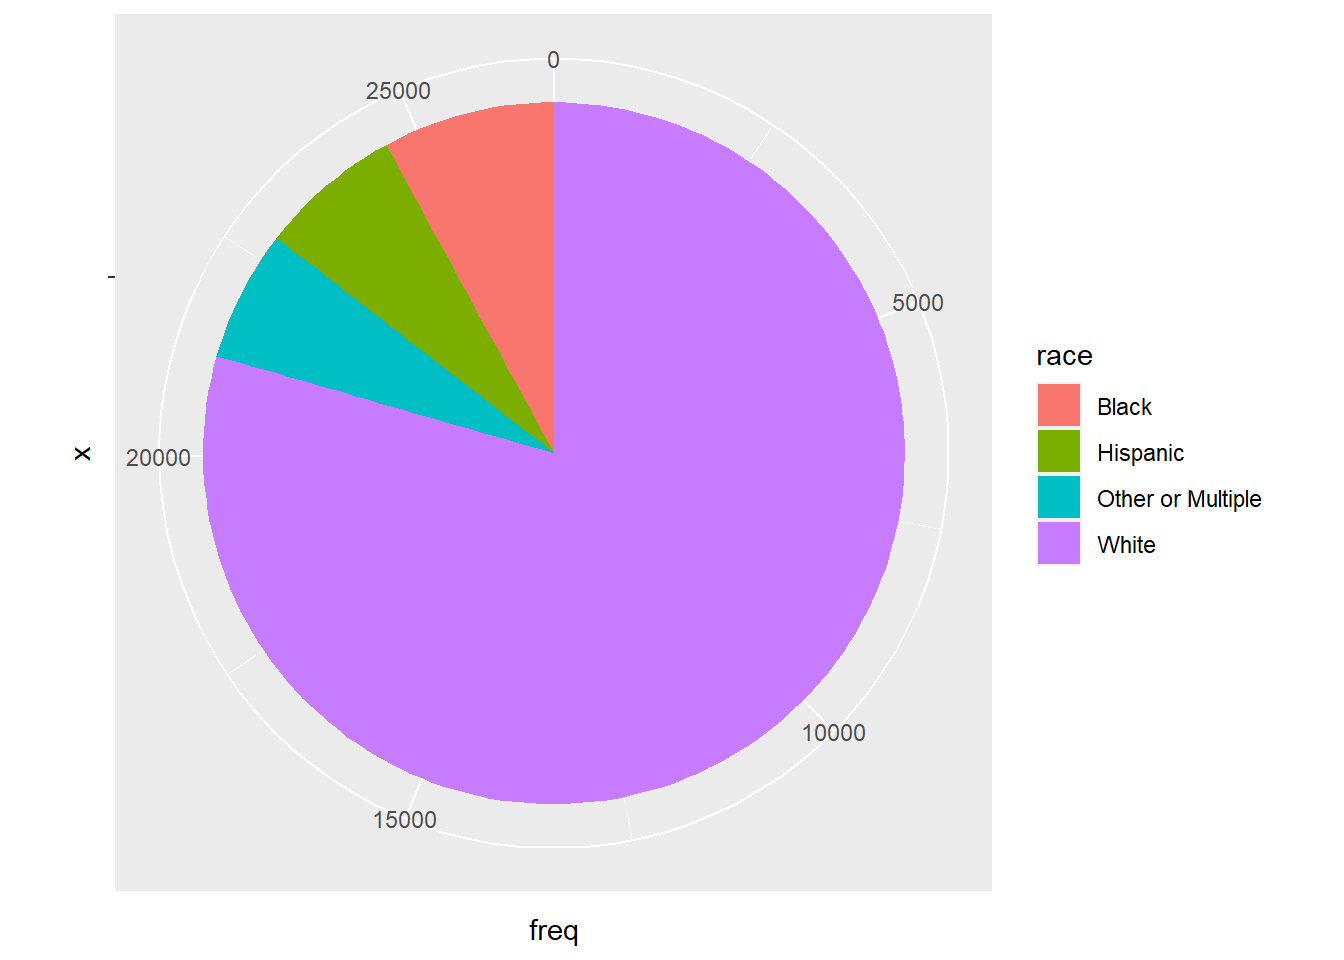
\includegraphics{RLearning_files/figure-latex/plot14-1.pdf}

看起来像饼图了,但是饼图周围还有多余的数字,如何清除呢?
这里的标签其实就是坐标轴的标签,可以通过labs()函数将其清除。

\begin{lstlisting}[language=R]
ggplot(data = data, aes(x = "", y = freq, fill = race)) +
  geom_bar(stat = "identity") +
  coord_polar(theta = "y") +
  labs(x = "", y = "", title = "") +
  theme(axis.text = element_blank())
\end{lstlisting}

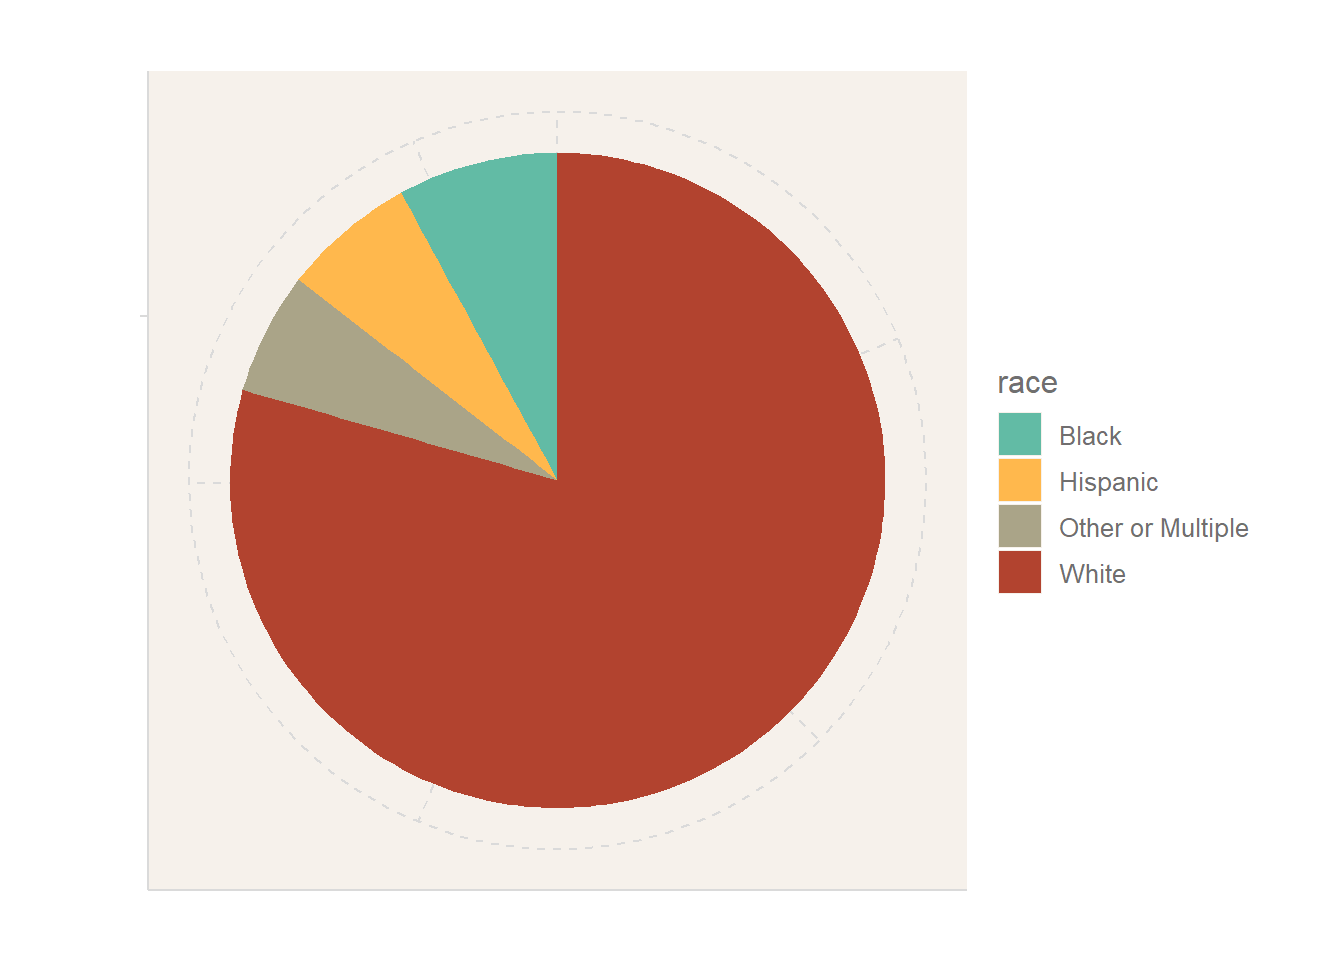
\includegraphics{RLearning_files/figure-latex/plot15-1.pdf}

接下来就是显示各个所占的比例
第一种方法,将百分比直接显示在图例中,这种方式适合分类较多的情况。

\begin{lstlisting}[language=R]
label_value <- paste("(", round(data$freq / sum(data$freq) * 100, 1), "%)", sep = "")
label_value
\end{lstlisting}

\begin{lstlisting}
## [1] "(7.9%)"  "(6.6%)"  "(6%)"    "(79.5%)"
\end{lstlisting}

将计算的百分比和race匹配

\begin{lstlisting}[language=R]
label <- paste(data$race, label_value, sep = "")
label
\end{lstlisting}

\begin{lstlisting}
## [1] "Black(7.9%)"           "Hispanic(6.6%)"        "Other or Multiple(6%)"
## [4] "White(79.5%)"
\end{lstlisting}

接下来就是将这些百分比标签放到图例中

\begin{lstlisting}[language=R]
ggplot(data = data, aes(x = "", y = freq, fill = race)) +
  geom_bar(stat = "identity") +
  coord_polar(theta = "y") +
  labs(x = "", y = "", title = "") +
  theme(axis.text = element_blank()) +
  scale_fill_discrete(labels = label)
\end{lstlisting}

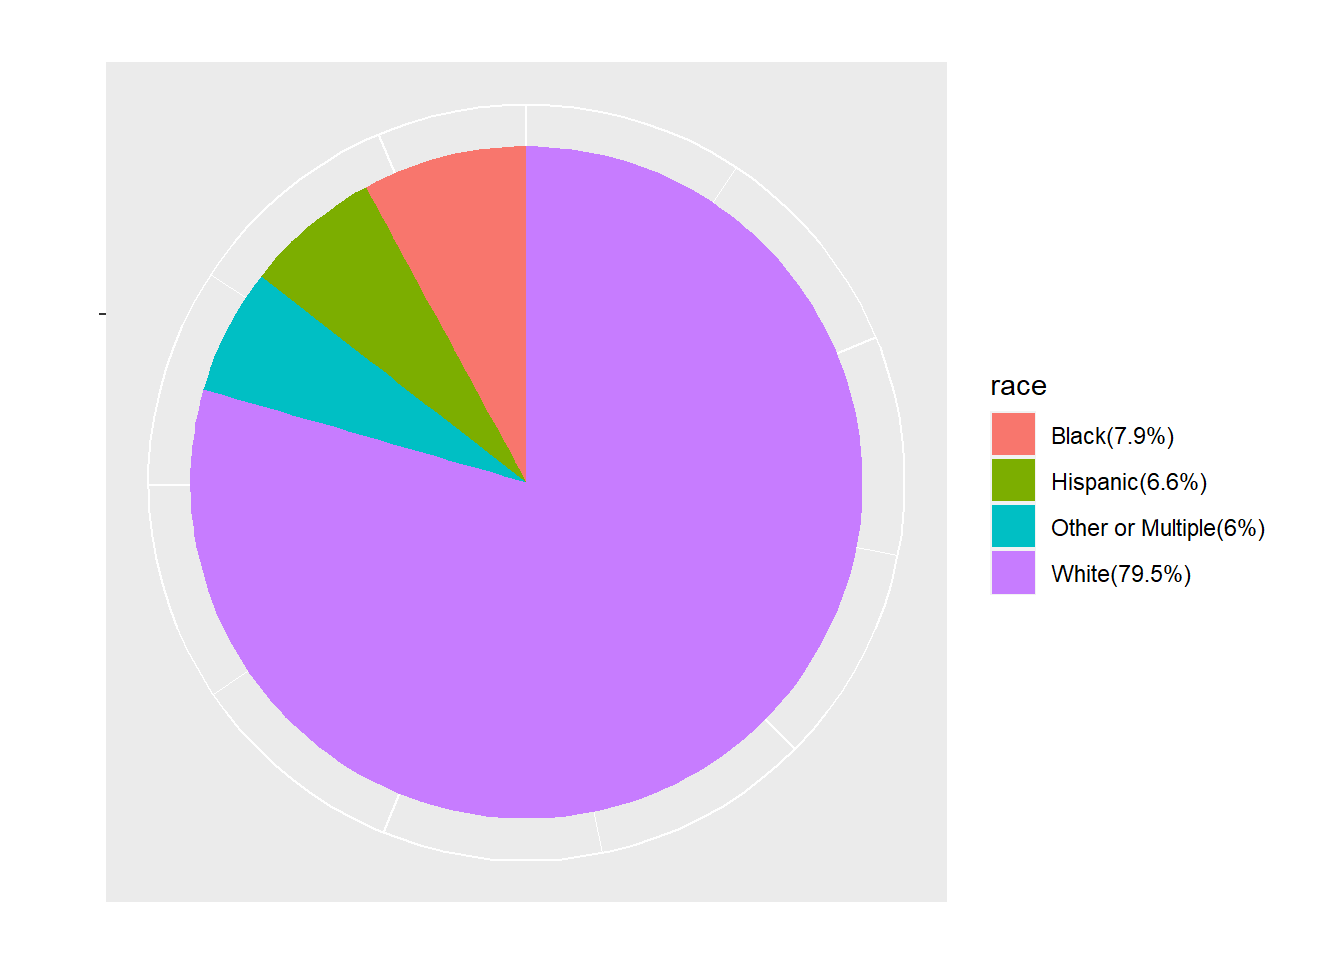
\includegraphics{RLearning_files/figure-latex/unnamed-chunk-125-1.pdf}

看起来就很不错\textasciitilde{}

第二种方法,直接将百分比放到各自的饼区中。

首先是去掉饼图中的图例

\begin{lstlisting}[language=R]
ggplot(data = data, aes(x = "", y = freq, fill = race)) +
  geom_bar(stat = "identity") +
  coord_polar(theta = "y") +
  labs(x = "", y = "", title = "") +
  theme(axis.text = element_blank()) +
  theme(legend.position = "none")
\end{lstlisting}

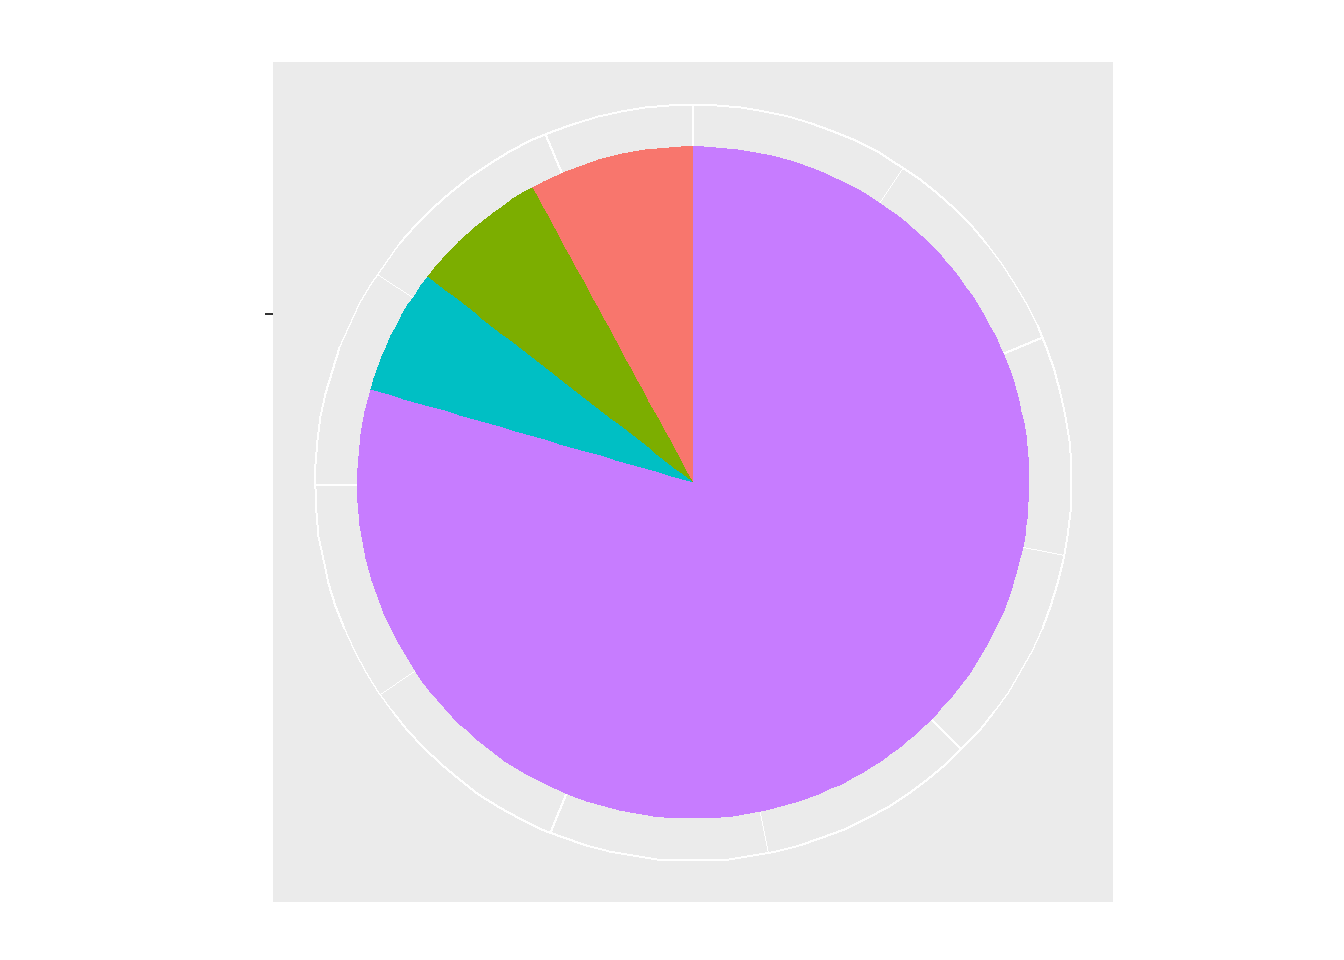
\includegraphics{RLearning_files/figure-latex/unnamed-chunk-126-1.pdf}

将标签放置在饼图中

\begin{lstlisting}[language=R]
ggplot(data = data, aes(x = "", y = freq, fill = race)) +
  geom_bar(stat = "identity", width = 1) +
  coord_polar(theta = "y") +
  labs(x = "", y = "", title = "") +
  theme(axis.text = element_blank(), legend.position = "none") +
  geom_text(aes(label = label), size = 3, position = position_stack(vjust = 0.5))
\end{lstlisting}

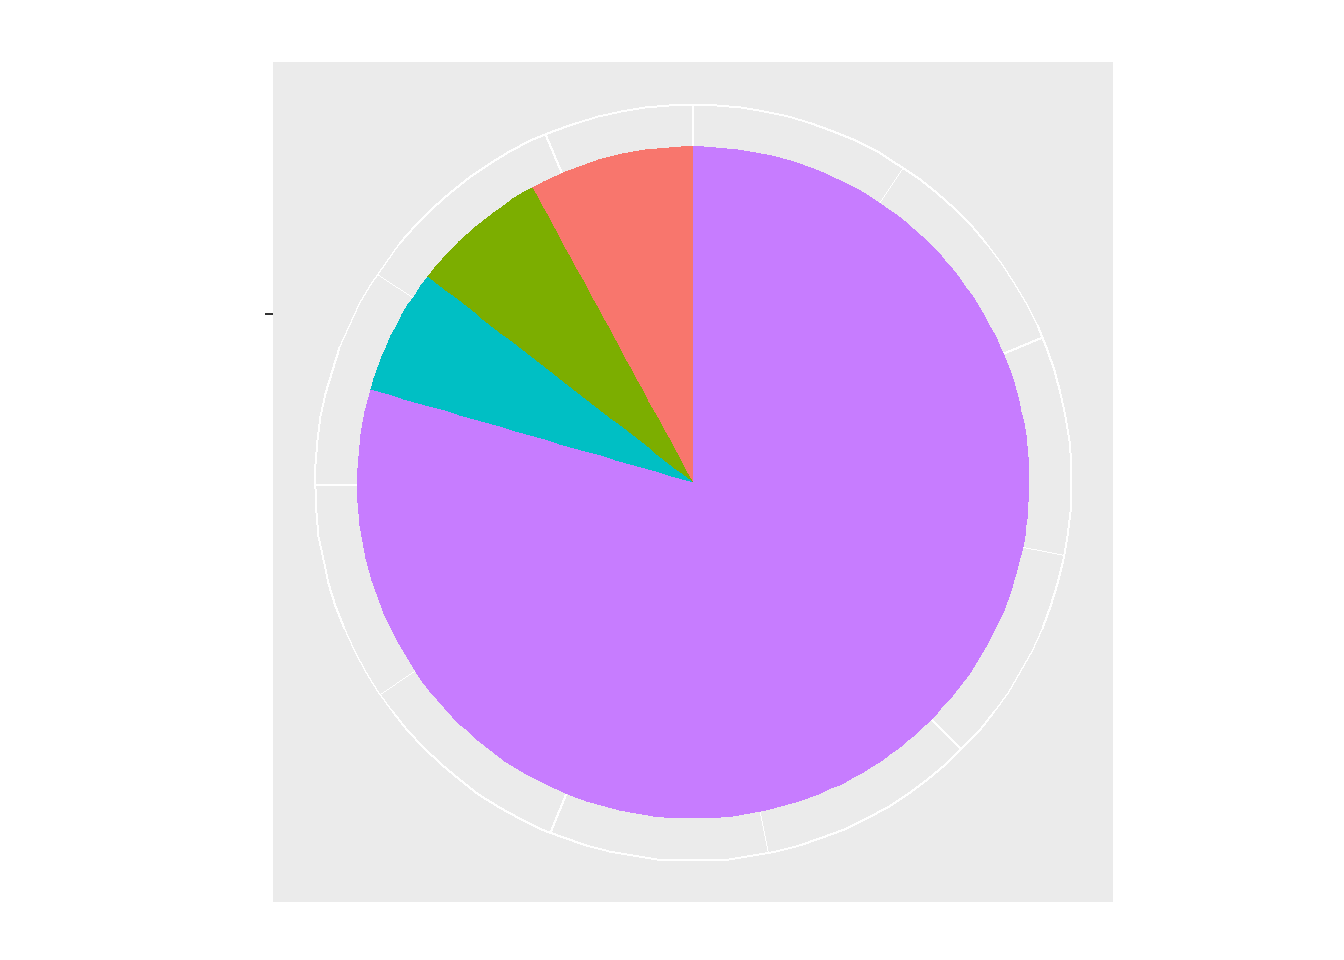
\includegraphics{RLearning_files/figure-latex/unnamed-chunk-127-1.pdf}

\hypertarget{ux6298ux7ebfux56fe}{%
\subsection{折线图}\label{ux6298ux7ebfux56fe}}

折线图作为反映数据变化的趋势是常用的数据可视化图形之一,在ggplot2中通过geom\_line()这个函数进行绘制。

对波士顿房价中rad进行可视化展示,使用pylr包中的count对edcation进行计数统计

\begin{lstlisting}[language=R]
data <- count(boston_data["rad"])
data
\end{lstlisting}

\begin{lstlisting}
##   rad freq
## 1   1   20
## 2   2   24
## 3   3   38
## 4   4  110
## 5   5  115
## 6   6   26
## 7   7   17
## 8   8   24
## 9  24  132
\end{lstlisting}

把rad为24的数据去除掉

\begin{lstlisting}[language=R]
data <- data[1:8, ]
ggplot(data, aes(x = rad, y = freq)) +
  geom_line()
\end{lstlisting}

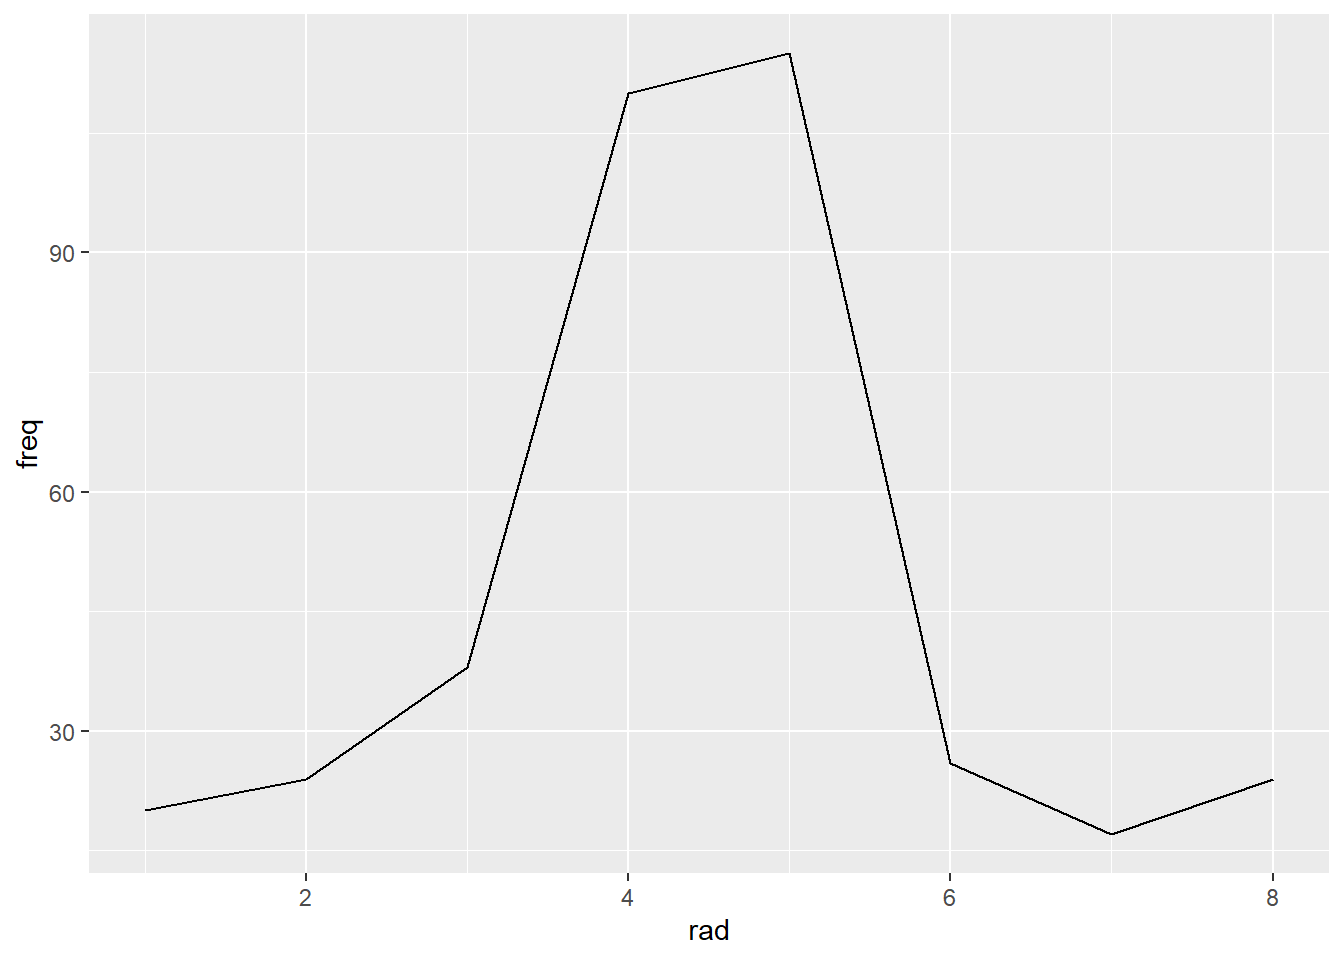
\includegraphics{RLearning_files/figure-latex/unnamed-chunk-129-1.pdf}

有时候我们需要在折线图上显示对应x轴的点数据,从而可以更加清晰的辨别原始数据,这特别适合数据比较稀疏的情况

\begin{lstlisting}[language=R]
ggplot(data, aes(x = rad, y = freq)) +
  geom_line() +
  geom_point(size = 4)
\end{lstlisting}

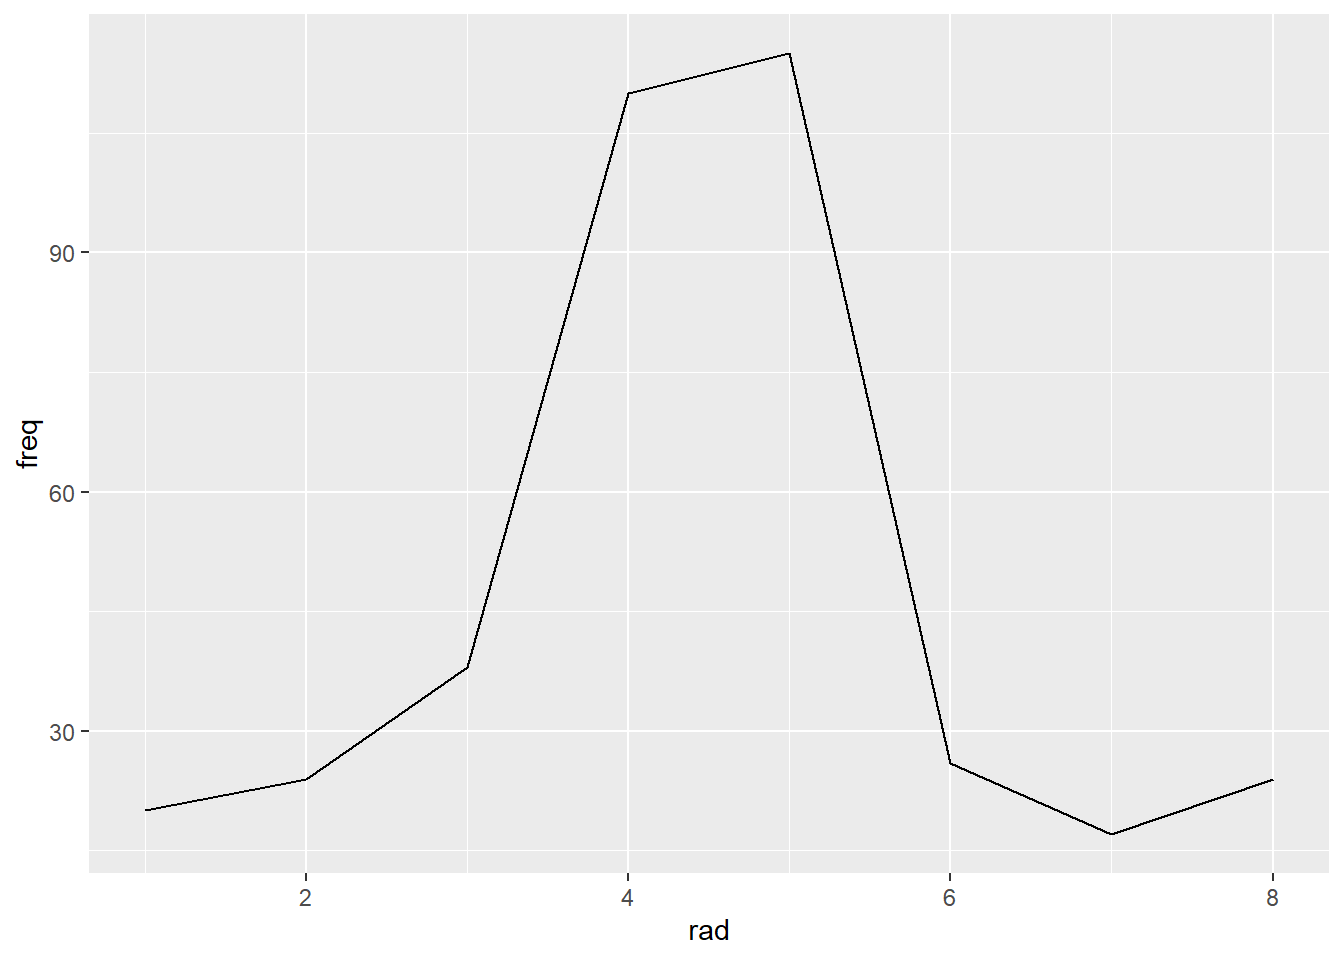
\includegraphics{RLearning_files/figure-latex/unnamed-chunk-130-1.pdf}

我们调整横坐标的显示刻度

\begin{lstlisting}[language=R]
ggplot(data, aes(x = rad, y = freq)) +
  geom_line() +
  geom_point(size = 4) +
  scale_x_continuous(breaks = c(1:8))
\end{lstlisting}

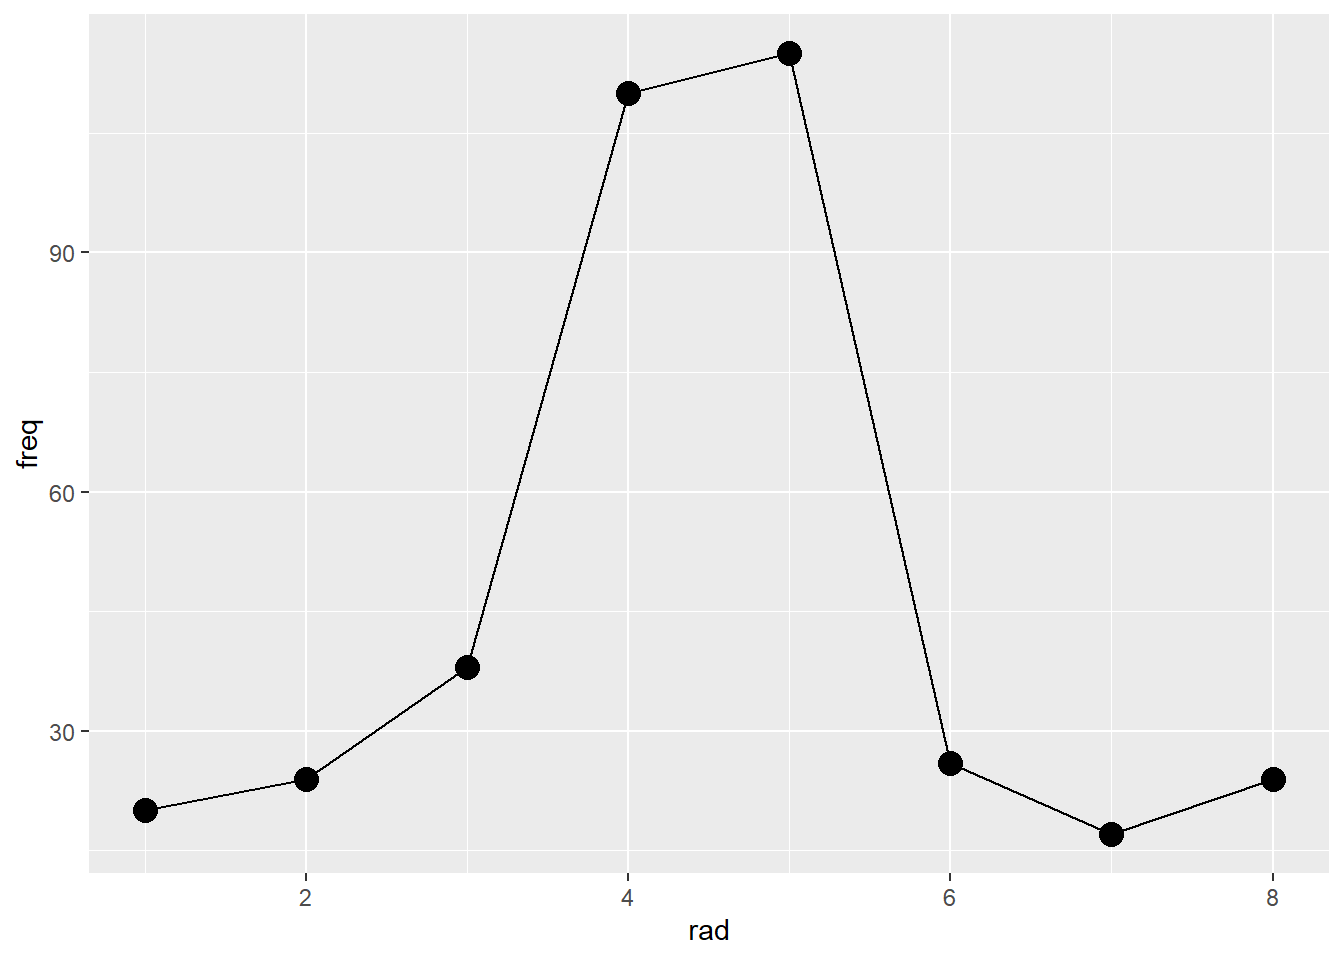
\includegraphics{RLearning_files/figure-latex/unnamed-chunk-131-1.pdf}

也可以修改线的类型和颜色

\begin{lstlisting}[language=R]
ggplot(data, aes(x = rad, y = freq)) +
  geom_line(linetype = "dashed", color = "red") +
  geom_point(size = 4) +
  scale_x_continuous(breaks = c(1:8))
\end{lstlisting}

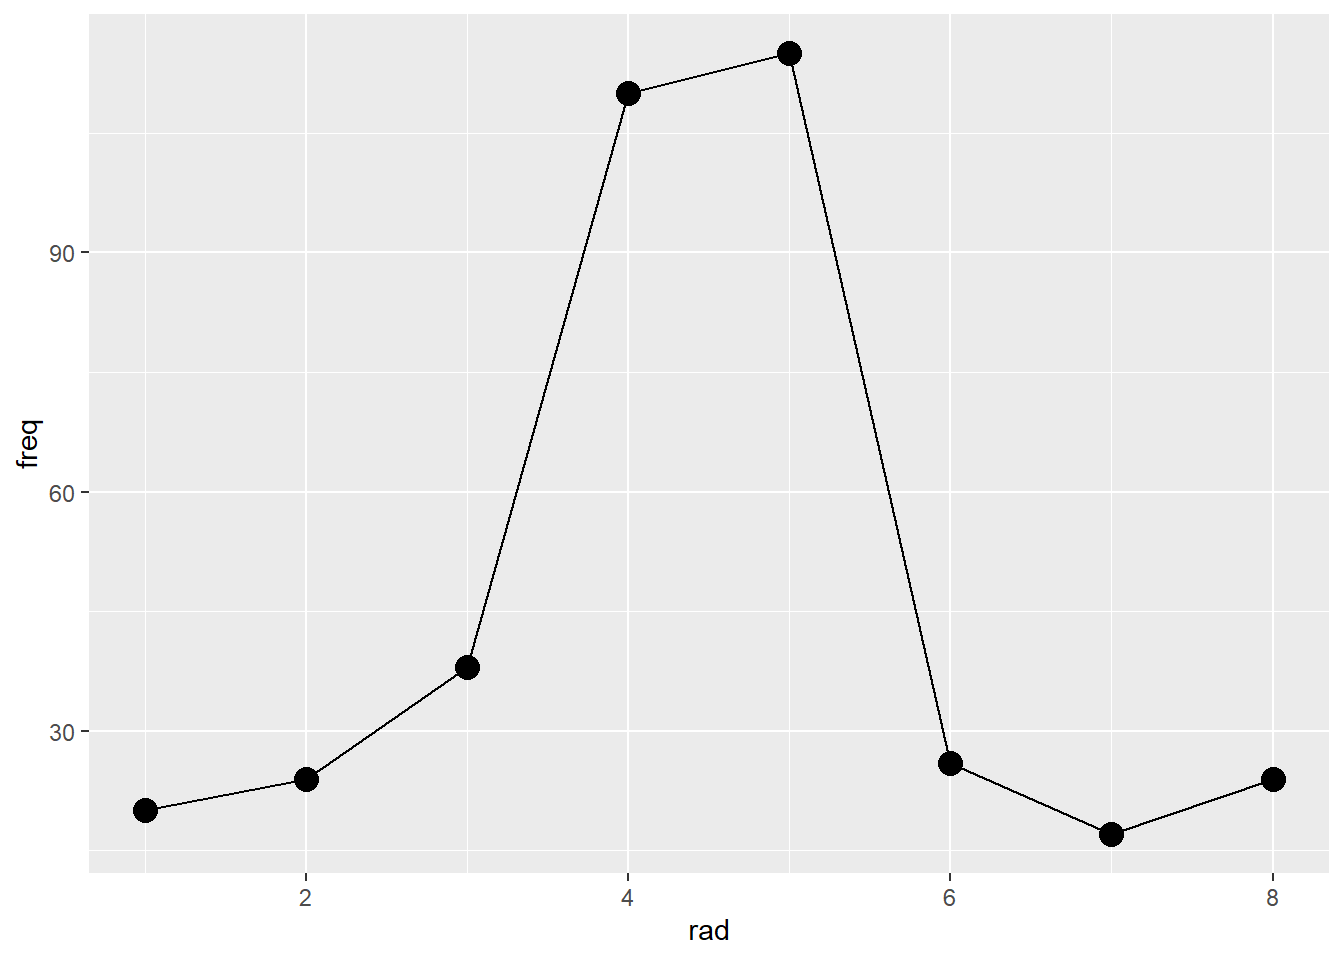
\includegraphics{RLearning_files/figure-latex/unnamed-chunk-132-1.pdf}

ggplt2关于折线图的相关做法的参考链接:
\url{https://ggplot2.tidyverse.org/reference/geom_abline.html}

\hypertarget{ggplot2ux6269ux5c55ux5305ux4e3bux9898}{%
\subsection{ggplot2扩展包主题}\label{ggplot2ux6269ux5c55ux5305ux4e3bux9898}}

R语言中的ggplot2包里面的风格固定,在需要特殊的图形时,需要更改甚至自定义设置主题。
ggplot2内置了8种风格的主题

\begin{longtable}[]{@{}ll@{}}
\toprule
主题函数 & 效果 \\
\midrule
\endhead
theme\_bw() & 网格白色主题 \\
theme\_classic() & 经典主题 \\
theme\_dark() & 暗色主题,可用于对比 \\
theme\_gray() & 默认主题 \\
theme\_light() & 浅色坐标带网格 \\
theme\_linedraw() & 黑色网格线 \\
theme\_minimal() & 极简主题 \\
theme\_void() & 空白主题 \\
\bottomrule
\end{longtable}

我们来试一试不同的主题

\begin{lstlisting}[language=R]
p <- ggplot(data = boston_data, aes(x = lstat, y = medv, colour = rad)) +
  geom_point()
p1 <- p + theme_bw() + labs(title = "网格白色主题") + theme(legend.position = "none")
p2 <- p + theme_classic() + labs(title = "经典主题") + theme(legend.position = "none")
p3 <- p + theme_dark() + labs(title = "暗色主题") + theme(legend.position = "none")
p4 <- p + theme_gray() + labs(title = "默认主题") + theme(legend.position = "none")
p5 <- p + theme_light() + labs(title = "浅色坐标带网格") + theme(legend.position = "none")
p6 <- p + theme_linedraw() + labs(title = "黑色网格线") + theme(legend.position = "none")
p7 <- p + theme_minimal() + labs(title = "极简主题") + theme(legend.position = "none")
p8 <- p + theme_void() + labs(title = "空白主题") + theme(legend.position = "none")

ggarrange(p1, p2, p3, p4, p5, p6, p7, p8, ncol = 4, nrow = 2, heights = 1.2)
\end{lstlisting}

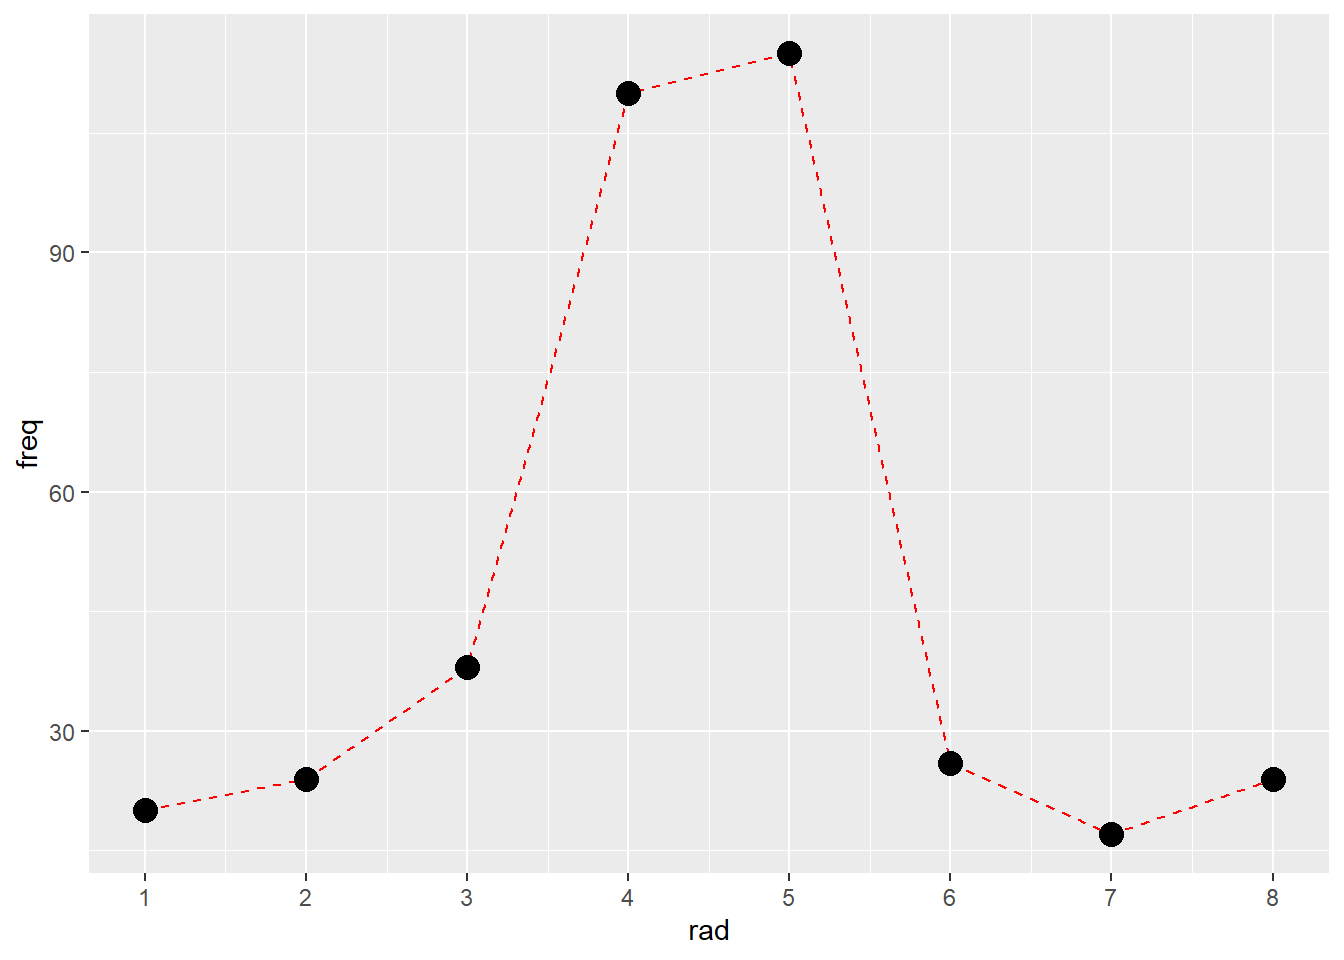
\includegraphics{RLearning_files/figure-latex/unnamed-chunk-133-1.pdf}

除了ggplot2自带的主题外,还有许多拓展主题包,比如:ggthemes、ggthemr
ggthemes在cran上发布,因此推荐使用这个
ggthemr 色彩很好看,因此推荐这个

ggthemes相关链接:\url{https://github.com/jrnold/ggthemes}

ggthemr相关链接:\url{https://github.com/Mikata-Project/ggthemr}

因为ggthemr没有上cran,因此需要通过github安装

\begin{lstlisting}[language=R]
# devtools::install_github('Mikata-Project/ggthemr')
\end{lstlisting}

使用方法也是非常简单,这里用我比较喜欢的greyscale主题方案

\begin{lstlisting}[language=R]
library(ggthemr)
ggthemr("greyscale")
p3 <- ggplot(data = boston_data, aes(x = lstat, y = medv, colour = factor(rad))) +
  geom_point()
p4 <- ggplot(data = boston_data, aes(x = lstat, y = medv, colour = rad)) +
  geom_point()
ggarrange(p3, p4, nrow = 1)
\end{lstlisting}

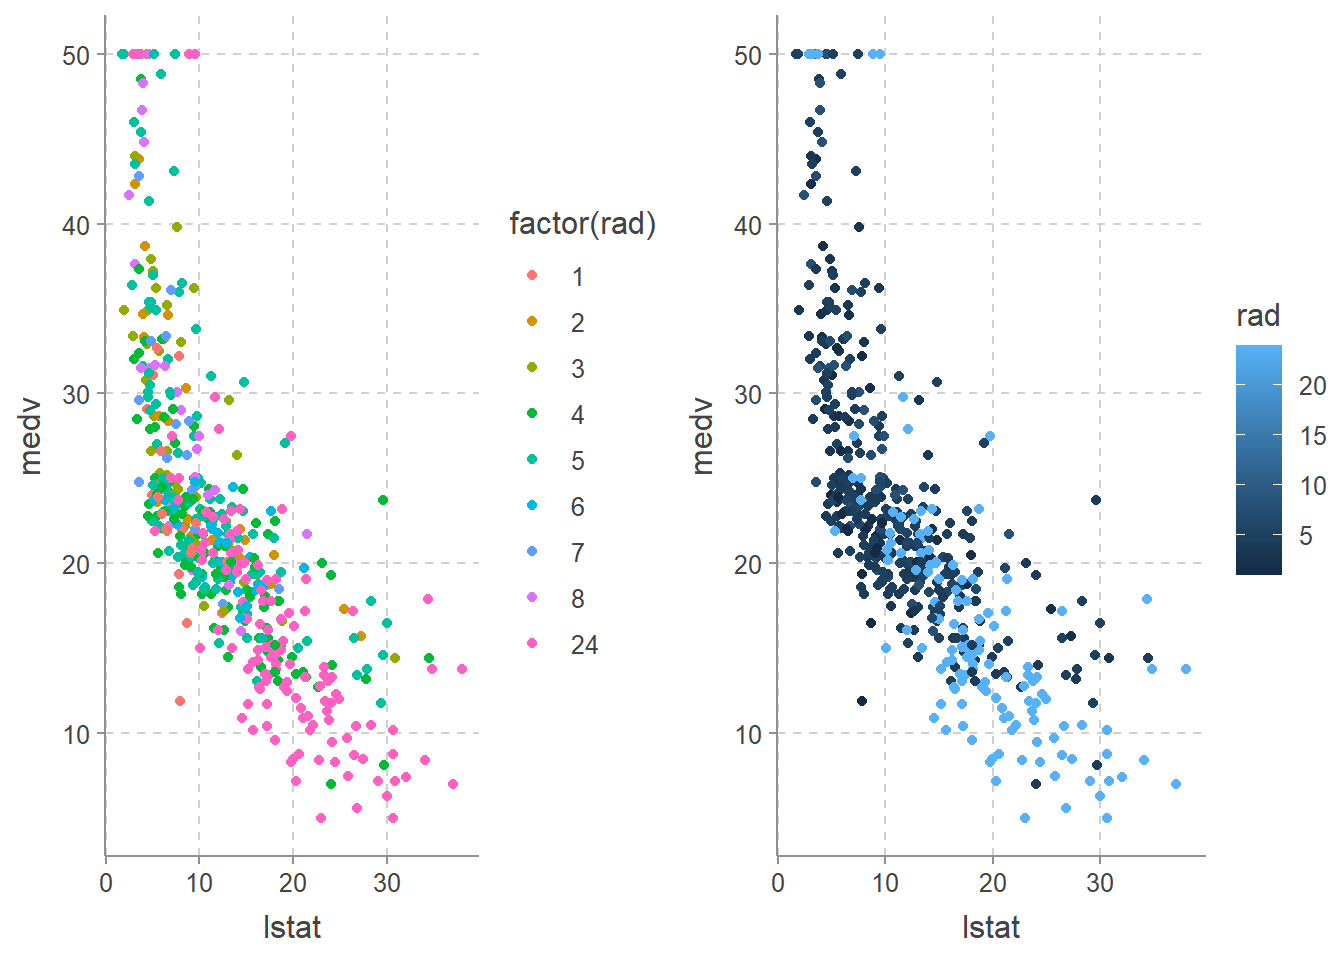
\includegraphics{RLearning_files/figure-latex/unnamed-chunk-135-1.pdf}

试一试light这个主题,配色非常的温柔

\begin{lstlisting}[language=R]
library(ggthemr)
ggthemr("light")
p3 <- ggplot(data = boston_data, aes(x = lstat, y = medv, colour = factor(rad))) +
  geom_point()
p4 <- ggplot(data = boston_data, aes(x = lstat, y = medv, colour = rad)) +
  geom_point()
ggarrange(p3, p4, nrow = 1)
\end{lstlisting}

\includegraphics{RLearning_files/figure-latex/unnamed-chunk-136-1.pdf}

实战部分:
对提供的数据集我们可以试一试ggthemr中的不同主题,同时对波士顿房价进行其它的数据可视化的探索。

ggplot2是一个非常经典的数据可视化R包,内容非常丰富,由于篇幅的原因没办法将ggplot2中的各种方法全部讲述,因此选择了几个常见的图形进行相关的讲解,以期达到抛砖引玉的效果。如果对ggplot2感兴趣的同学,可以去官网进行更加详细的学习,也非常期待大家的数据可视化作品\textasciitilde{}

\hypertarget{ux672cux7ae0ux4f5cux8005-4}{%
\subsection*{本章作者}\label{ux672cux7ae0ux4f5cux8005-4}}


\textbf{牧小熊}

\begin{quote}
华中农业大学研究生,Datawhale成员, Datawhale优秀原创作者\\
知乎:\url{https://www.zhihu.com/people/muxiaoxiong}
\end{quote}

\hypertarget{ux5173ux4e8edatawhale-4}{%
\subsection*{关于Datawhale}\label{ux5173ux4e8edatawhale-4}}


Datawhale是一个专注于数据科学与AI领域的开源组织,汇集了众多领域院校和知名企业的优秀学习者,聚合了一群有开源精神和探索精神的团队成员。Datawhale 以``for the learner,和学习者一起成长''为愿景,鼓励真实地展现自我、开放包容、互信互助、敢于试错和勇于担当。同时 Datawhale 用开源的理念去探索开源内容、开源学习和开源方案,赋能人才培养,助力人才成长,建立起人与人,人与知识,人与企业和人与未来的联结。 本次数据挖掘路径学习,专题知识将在天池分享,详情可关注Datawhale:

\includegraphics[width=3.58in]{image/logo}

\hypertarget{task-05}{%
\section{模型}\label{task-05}}

\includegraphics[width=1\textwidth,height=\textheight]{./image/task05_structure.png}

Task05共计3个知识点,预计需学习2-3小时,请安排好学习任务。

\hypertarget{ux524dux8a00}{%
\subsection{前言}\label{ux524dux8a00}}

为了帮助大家更好的使用R语言进行建模分析,本章节将借助波士顿房价数据集来展示常见的模型。本章节学习的目的是帮助大家了解模型的适用范围以及如何建模,不会对模型的底层原理进行深入的研究。并且迫于时间和精力有限,本章节仅介绍部分模型的实现。

\begin{itemize}
\item
  回归模型: 回归模型是一种有监督的、预测性的建模技术,它研究的是因变量和自变量之间的关系。
\item
  分类模型: 分类模型也是一种有监督的机器学习模型。与回归模型不同的是,其标签(因变量)通常是有限个数的定类变量。最常见的是二分类模型。
\end{itemize}

我们主要使用波士顿房价数据集来实现各种模型。因此我们使用2021作为种子值生成70\%的数据作为训练集,其余数据作为测试集。下面展示来各个数据集的大小。

\begin{lstlisting}[language=R]
# 导入BostonHousing数据
library(mlbench)
data(BostonHousing)

# 设置种子值,方便复现
set.seed(2021)

# 生成训练集的索引,用来划分训练集和测试集
train_index <- sample(dim(BostonHousing)[1], 0.7 * dim(BostonHousing)[1])
BostonHousingTrain <- BostonHousing[train_index, ]
BostonHousingTest <- BostonHousing[-train_index, ]

# 查看数据集的size
dim(BostonHousing)
\end{lstlisting}

\begin{lstlisting}
## [1] 506  14
\end{lstlisting}

\begin{lstlisting}[language=R]
dim(BostonHousingTrain)
\end{lstlisting}

\begin{lstlisting}
## [1] 354  14
\end{lstlisting}

\begin{lstlisting}[language=R]
dim(BostonHousingTest)
\end{lstlisting}

\begin{lstlisting}
## [1] 152  14
\end{lstlisting}

\begin{lstlisting}[language=R]
# 查看数据集包含的变量名称
names(BostonHousing)
\end{lstlisting}

\begin{lstlisting}
##  [1] "crim"    "zn"      "indus"   "chas"    "nox"     "rm"      "age"    
##  [8] "dis"     "rad"     "tax"     "ptratio" "b"       "lstat"   "medv"
\end{lstlisting}

\#\#回归模型
回归模型有很多主要有Linear Regression、Logistic Regression、Polynomial Regression、Stepwise Regression、Ridge Regression、Lasso Regression、ElasticNet等。

本部分主要介绍有Linear Regression、以及Stepwise Regression三种回归模型的实现。

\hypertarget{linear-regression}{%
\subsubsection{Linear Regression}\label{linear-regression}}

多元线性回归是一种最为基础的回归模型,其使用多个自变量和一个因变量利用OLS完成模型训练。下面我们将使用\passthrough{\lstinline!medv!}作为因变量,剩余变量作为自变量构建模型。

多元线性回归模型使用\passthrough{\lstinline!lm()!}命令, 其中\passthrough{\lstinline!medv\~.!}是回归公式,\passthrough{\lstinline!data=BostonHousingTrain!}是回归数据。对回归公式的构建进行一些补充,\passthrough{\lstinline!\~!}左侧表示因变量,\passthrough{\lstinline!\~!}右侧表示自变量,多个自变量使用\passthrough{\lstinline!+!}依次叠加。这里右侧使用了\passthrough{\lstinline!.!},该符号的含义是除左侧变量外所有的变量。因此,\passthrough{\lstinline!medv\~.!}等价于\passthrough{\lstinline!medv\~crim + zn + indus + chas + nox + rm + age + dis + rad + tax + ptratio + b + medv!}。

\begin{lstlisting}[language=R]
# 构建模型,medv~.表示回归方程
lr_model <- lm(medv ~ ., data = BostonHousingTrain)

# summary输出模型汇总
summary(lr_model)
\end{lstlisting}

\begin{lstlisting}
## 
## Call:
## lm(formula = medv ~ ., data = BostonHousingTrain)
## 
## Residuals:
##      Min       1Q   Median       3Q      Max 
## -17.1929  -2.6567  -0.3854   1.6261  28.5425 
## 
## Coefficients:
##               Estimate Std. Error t value Pr(>|t|)    
## (Intercept)  28.279554   6.464743   4.374 1.62e-05 ***
## crim         -0.066574   0.051496  -1.293 0.196958    
## zn            0.031466   0.016525   1.904 0.057733 .  
## indus         0.046583   0.069009   0.675 0.500115    
## chas1         3.372501   1.065312   3.166 0.001687 ** 
## nox         -14.103937   4.498414  -3.135 0.001866 ** 
## rm            4.512687   0.547845   8.237 3.85e-15 ***
## age          -0.010015   0.016016  -0.625 0.532197    
## dis          -1.259008   0.245311  -5.132 4.82e-07 ***
## rad           0.263841   0.077147   3.420 0.000702 ***
## tax          -0.012026   0.004176  -2.880 0.004235 ** 
## ptratio      -1.008997   0.160048  -6.304 8.99e-10 ***
## b             0.014361   0.003406   4.217 3.18e-05 ***
## lstat        -0.466948   0.062026  -7.528 4.66e-13 ***
## ---
## Signif. codes:  0 '***' 0.001 '**' 0.01 '*' 0.05 '.' 0.1 ' ' 1
## 
## Residual standard error: 4.776 on 340 degrees of freedom
## Multiple R-squared:  0.7299, Adjusted R-squared:  0.7196 
## F-statistic: 70.67 on 13 and 340 DF,  p-value: < 2.2e-16
\end{lstlisting}

运用plot命令对模型进行诊断,各图含义参考 \url{https://www.cnblogs.com/lafengdatascientist/p/5554167.html}

\begin{lstlisting}[language=R]
plot(lr_model)
\end{lstlisting}

\includegraphics{RLearning_files/figure-latex/unnamed-chunk-140-1.pdf} \includegraphics{RLearning_files/figure-latex/unnamed-chunk-140-2.pdf} \includegraphics{RLearning_files/figure-latex/unnamed-chunk-140-3.pdf} \includegraphics{RLearning_files/figure-latex/unnamed-chunk-140-4.pdf}

\passthrough{\lstinline!predict!}命令能够基于已经训练好的模型进行预测。

\begin{lstlisting}[language=R]
# 根据模型对新数据进行预测
BostonHousingTest$lr_pred <- predict(lr_model, newdata = BostonHousingTest)
\end{lstlisting}

\hypertarget{stepwise-regression}{%
\subsubsection{Stepwise Regression}\label{stepwise-regression}}

利用逐步回归分析可以对模型中的变量进行优化。R语言中的\passthrough{\lstinline!step()!}命令,是以AIC信息统计量为准则,通过选择最小的AIC信息统计量来达到提出或添加变量的目的。

对于逐步回归,一般有前向、后向、双向等逐步方式。本部分将基于已经实现的\passthrough{\lstinline!lr\_model!}进行双向逐步回归。前向和后向回归只需要更改\passthrough{\lstinline!step()!}命令行中的\passthrough{\lstinline!direstion!}参数即可。具体内容参照 \url{https://blog.csdn.net/qq_38204302/article/details/86567356}

\begin{lstlisting}[language=R]
# both逐步回归
step_model <- step(lr_model, direction = "both")
\end{lstlisting}

\begin{lstlisting}
## Start:  AIC=1120.78
## medv ~ crim + zn + indus + chas + nox + rm + age + dis + rad + 
##     tax + ptratio + b + lstat
## 
##           Df Sum of Sq    RSS    AIC
## - age      1      8.92 7765.1 1119.2
## - indus    1     10.39 7766.6 1119.3
## - crim     1     38.13 7794.3 1120.5
## <none>                 7756.2 1120.8
## - zn       1     82.71 7838.9 1122.5
## - tax      1    189.16 7945.4 1127.3
## - nox      1    224.25 7980.5 1128.9
## - chas     1    228.62 7984.8 1129.1
## - rad      1    266.82 8023.0 1130.8
## - b        1    405.60 8161.8 1136.8
## - dis      1    600.89 8357.1 1145.2
## - ptratio  1    906.67 8662.9 1157.9
## - lstat    1   1292.88 9049.1 1173.4
## - rm       1   1547.84 9304.0 1183.2
## 
## Step:  AIC=1119.19
## medv ~ crim + zn + indus + chas + nox + rm + dis + rad + tax + 
##     ptratio + b + lstat
## 
##           Df Sum of Sq    RSS    AIC
## - indus    1     10.22 7775.3 1117.7
## - crim     1     39.31 7804.4 1119.0
## <none>                 7765.1 1119.2
## + age      1      8.92 7756.2 1120.8
## - zn       1     92.34 7857.5 1121.4
## - tax      1    193.70 7958.8 1125.9
## - chas     1    225.98 7991.1 1127.3
## - nox      1    261.86 8027.0 1128.9
## - rad      1    278.77 8043.9 1129.7
## - b        1    398.83 8164.0 1134.9
## - dis      1    613.30 8378.4 1144.1
## - ptratio  1    916.06 8681.2 1156.7
## - lstat    1   1546.55 9311.7 1181.5
## - rm       1   1571.42 9336.5 1182.4
## 
## Step:  AIC=1117.65
## medv ~ crim + zn + chas + nox + rm + dis + rad + tax + ptratio + 
##     b + lstat
## 
##           Df Sum of Sq    RSS    AIC
## - crim     1     41.19 7816.5 1117.5
## <none>                 7775.3 1117.7
## + indus    1     10.22 7765.1 1119.2
## + age      1      8.74 7766.6 1119.3
## - zn       1     88.58 7863.9 1119.7
## - tax      1    189.88 7965.2 1124.2
## - chas     1    231.63 8007.0 1126.0
## - nox      1    252.32 8027.7 1127.0
## - rad      1    269.59 8044.9 1127.7
## - b        1    395.78 8171.1 1133.2
## - dis      1    706.93 8482.3 1146.5
## - ptratio  1    906.25 8681.6 1154.7
## - lstat    1   1537.69 9313.0 1179.5
## - rm       1   1561.38 9336.7 1180.4
## 
## Step:  AIC=1117.52
## medv ~ zn + chas + nox + rm + dis + rad + tax + ptratio + b + 
##     lstat
## 
##           Df Sum of Sq    RSS    AIC
## <none>                 7816.5 1117.5
## + crim     1     41.19 7775.3 1117.7
## + indus    1     12.10 7804.4 1119.0
## - zn       1     76.92 7893.5 1119.0
## + age      1      9.92 7806.6 1119.1
## - tax      1    182.40 7998.9 1123.7
## - rad      1    228.86 8045.4 1125.7
## - nox      1    236.90 8053.4 1126.1
## - chas     1    240.06 8056.6 1126.2
## - b        1    514.43 8331.0 1138.1
## - dis      1    673.74 8490.3 1144.8
## - ptratio  1    893.27 8709.8 1153.8
## - lstat    1   1589.98 9406.5 1181.1
## - rm       1   1636.60 9453.1 1182.8
\end{lstlisting}

\begin{lstlisting}[language=R]
summary(step_model)
\end{lstlisting}

\begin{lstlisting}
## 
## Call:
## lm(formula = medv ~ zn + chas + nox + rm + dis + rad + tax + 
##     ptratio + b + lstat, data = BostonHousingTrain)
## 
## Residuals:
##      Min       1Q   Median       3Q      Max 
## -16.8955  -2.6773  -0.4005   1.6707  28.5842 
## 
## Coefficients:
##               Estimate Std. Error t value Pr(>|t|)    
## (Intercept)  27.001770   6.354437   4.249 2.77e-05 ***
## zn            0.029797   0.016219   1.837  0.06705 .  
## chas1         3.446516   1.061891   3.246  0.00129 ** 
## nox         -13.578105   4.211269  -3.224  0.00138 ** 
## rm            4.491255   0.529976   8.474 7.07e-16 ***
## dis          -1.213451   0.223170  -5.437 1.03e-07 ***
## rad           0.220392   0.069546   3.169  0.00167 ** 
## tax          -0.010818   0.003824  -2.829  0.00494 ** 
## ptratio      -0.991885   0.158427  -6.261 1.14e-09 ***
## b             0.015446   0.003251   4.751 2.98e-06 ***
## lstat        -0.482234   0.057733  -8.353 1.67e-15 ***
## ---
## Signif. codes:  0 '***' 0.001 '**' 0.01 '*' 0.05 '.' 0.1 ' ' 1
## 
## Residual standard error: 4.774 on 343 degrees of freedom
## Multiple R-squared:  0.7278, Adjusted R-squared:  0.7199 
## F-statistic: 91.71 on 10 and 343 DF,  p-value: < 2.2e-16
\end{lstlisting}

对于分类模型还有较为常用的Lasso Regression 和 Ridge Regression,我们将会在进阶教程中来更加具体的讲解模型知识。

\hypertarget{ux5206ux7c7bux6a21ux578b}{%
\subsection{分类模型}\label{ux5206ux7c7bux6a21ux578b}}

在进行分类模型前,我们需要构建分类标签。我们使用\passthrough{\lstinline!medv!}的中位数进行划分,其中1表示高房价,0表示低房价。通过这样的转化将原本的数值型变量转化为二元标签。并使用相同的种子值划分测试集和训练集。

\begin{lstlisting}[language=R]
# 将连续变量转化成二分类变量
BostonHousing$medv <- as.factor(ifelse(BostonHousing$medv > median(BostonHousing$medv), 1, 0))
# 查看两种变量类别的数量
summary(BostonHousing$medv)
\end{lstlisting}

\begin{lstlisting}
##   0   1 
## 256 250
\end{lstlisting}

\begin{lstlisting}[language=R]
# 使用相同的种子值,复现训练集合测试集的划分
set.seed(2021)
train_index <- sample(dim(BostonHousing)[1], 0.7 * dim(BostonHousing)[1])
BostonHousingTrain <- BostonHousing[train_index, ]
BostonHousingTest <- BostonHousing[-train_index, ]
\end{lstlisting}

同时引入两个计算函数,用来计算AUC指标值。

\begin{lstlisting}[language=R]
# 引入auc计算函数
library("ROCR")
calcAUC <- function(predcol, outcol) {
  perf <- performance(prediction(predcol, outcol == 1), "auc")
  as.numeric(perf@y.values)
}
\end{lstlisting}

\hypertarget{logistics-regression}{%
\subsubsection{Logistics Regression}\label{logistics-regression}}

逻辑回归是一种广义的线性回归分析模型,利用sigmode将线性回归结果转化成概率的形式。下面展示了利用\passthrough{\lstinline!glm()!}构建逻辑回归的过程。通过计算,训练集上的auc取值为0.9554211,测试集上的auc取值为0.9506969,说明模型效果整体不错。

\begin{lstlisting}[language=R]
# 逻辑回归模型构建
lr_model <- glm(medv ~ ., data = BostonHousingTrain, family = binomial(link = "logit"))
summary(lr_model)
\end{lstlisting}

\begin{lstlisting}
## 
## Call:
## glm(formula = medv ~ ., family = binomial(link = "logit"), data = BostonHousingTrain)
## 
## Deviance Residuals: 
##      Min        1Q    Median        3Q       Max  
## -2.00065  -0.34945  -0.01094   0.24116   3.00080  
## 
## Coefficients:
##              Estimate Std. Error z value Pr(>|z|)    
## (Intercept)  4.641164   4.937497   0.940 0.347226    
## crim        -0.053419   0.096982  -0.551 0.581760    
## zn           0.005680   0.015218   0.373 0.708951    
## indus        0.045677   0.048167   0.948 0.342973    
## chas1        1.634949   0.798937   2.046 0.040717 *  
## nox         -6.916586   3.286514  -2.105 0.035332 *  
## rm           2.876778   0.651573   4.415 1.01e-05 ***
## age         -0.034146   0.013493  -2.531 0.011383 *  
## dis         -0.696695   0.209391  -3.327 0.000877 ***
## rad          0.220168   0.074211   2.967 0.003009 ** 
## tax         -0.009724   0.003446  -2.822 0.004769 ** 
## ptratio     -0.611081   0.132894  -4.598 4.26e-06 ***
## b            0.006135   0.003830   1.602 0.109159    
## lstat       -0.267857   0.064765  -4.136 3.54e-05 ***
## ---
## Signif. codes:  0 '***' 0.001 '**' 0.01 '*' 0.05 '.' 0.1 ' ' 1
## 
## (Dispersion parameter for binomial family taken to be 1)
## 
##     Null deviance: 489.83  on 353  degrees of freedom
## Residual deviance: 187.85  on 340  degrees of freedom
## AIC: 215.85
## 
## Number of Fisher Scoring iterations: 7
\end{lstlisting}

\begin{lstlisting}[language=R]
# 分别对训练集和测试集进行预测
lr_pred_train <- predict(lr_model, newdata = BostonHousingTrain, type = "response")
lr_pred_test <- predict(lr_model, newdata = BostonHousingTest, type = "response")

# 计算训练集和测试集的auc
calcAUC(lr_pred_train, BostonHousingTrain$medv)
\end{lstlisting}

\begin{lstlisting}
## [1] 0.9554211
\end{lstlisting}

\begin{lstlisting}[language=R]
calcAUC(lr_pred_test, BostonHousingTest$medv)
\end{lstlisting}

\begin{lstlisting}
## [1] 0.9506969
\end{lstlisting}

\hypertarget{knn}{%
\subsubsection{KNN}\label{knn}}

KNN模型是一种简单易懂、可以用于分类和回归的模型。其中 K 表示在新样本点附近(距离)选取 K 个样本数据,通过在 K 个样本进行投票来判断新增样本的类型。

KNN模型较难的一点是确定超参数K,目前有一些指标和经验方法帮助确定最优K的取值。这部分内容会在后续进行讲解,这里使用k=25进行建模。KNN模型在测试集上的auc值为0.8686411,相比于逻辑回归效果较差。

\begin{lstlisting}[language=R]
# 导入knn模型的包
library(kknn)

# 构建knn模型
knn <- kknn(medv ~ ., BostonHousingTrain, BostonHousingTest, k = 25)

# 预测并计算测试集上的auc取值
knn_pred_test <- predict(knn, newdata = BostonHousingTest)
calcAUC(as.numeric(knn_pred_test), BostonHousingTest$medv)
\end{lstlisting}

\begin{lstlisting}
## [1] 0.875784
\end{lstlisting}

\hypertarget{decision-tree}{%
\subsubsection{Decision Tree}\label{decision-tree}}

决策树是一种基于树模型进行划分的分类模型,通过一系列if then决策规则的集合,将特征空间划分成有限个不相交的子区域,对于落在相同子区域的样本,决策树模型给出相同的预测值。下面构建了决策树的分类模型

\begin{lstlisting}[language=R]
# 导入包
library(tree)

# 构建决策树模型函数,medv~.是决策树公式,用来表明变量。
# summary输出模型汇总信息
dt_model <- tree(medv ~ ., BostonHousingTrain)
summary(dt_model)
\end{lstlisting}

\begin{lstlisting}
## 
## Classification tree:
## tree(formula = medv ~ ., data = BostonHousingTrain)
## Variables actually used in tree construction:
##  [1] "lstat"   "rm"      "crim"    "ptratio" "b"       "tax"     "dis"    
##  [8] "age"     "nox"     "zn"     
## Number of terminal nodes:  20 
## Residual mean deviance:  0.2984 = 99.66 / 334 
## Misclassification error rate: 0.07062 = 25 / 354
\end{lstlisting}

\begin{lstlisting}[language=R]
# plot可以对树模型进行绘制,但可能会出现书分支过多的情况。
plot(dt_model)
text(dt_model)
\end{lstlisting}

\includegraphics{RLearning_files/figure-latex/unnamed-chunk-147-1.pdf}

在构建决策树模型的基础上,分别对训练集和测试集进行预测并计算auc取值。该模型在训练集上的auc取值为0.9281874,在测试集上的auc取值为0.8789199。训练集和测试集间存在抖动,说明该模型可能出现过拟合。我们需要引入剪枝的操作来降低模型的过拟合,这部分供同学们自学。

\begin{lstlisting}[language=R]
# 预测
dt_pred_train <- predict(dt_model, newdata = BostonHousingTrain, type = "class")
dt_pred_test <- predict(dt_model, newdata = BostonHousingTest, type = "class")

# 计算auc取值
calcAUC(as.numeric(dt_pred_train), BostonHousingTrain$medv)
\end{lstlisting}

\begin{lstlisting}
## [1] 0.9308756
\end{lstlisting}

\begin{lstlisting}[language=R]
calcAUC(as.numeric(dt_pred_test), BostonHousingTest$medv)
\end{lstlisting}

\begin{lstlisting}
## [1] 0.8789199
\end{lstlisting}

\hypertarget{random-forest}{%
\subsubsection{Random Forest}\label{random-forest}}

随机森林是一个包含多个决策树的分类器,可以用于分类和回归问题。在解决分类问题是,其输出的类别是由个别树输出的类别的众数而定。相比于单树模型,随机森林具有更好地泛化能力。

使用\passthrough{\lstinline!randomForest()!}构建模型的过程中,可以通过\passthrough{\lstinline!ntree!}设定随机森林中包含的决策树数量。由于随机森林是对样本和变量的随机,因此可以通过\passthrough{\lstinline!important!}展示变量的重要性排序。通过模型预测,随机森林模型在训练集上的auc为0.9615975,在测试集上的auc为0.9247387。

\begin{lstlisting}[language=R]
# 导入随机森林包
library(randomForest)

# 随机森林模型
rf_model <- randomForest(medv ~ ., BostonHousingTrain, ntree = 100, nodesize = 10, importance = T)
# 展示模型变量的重要性
importance(rf_model)
\end{lstlisting}

\begin{lstlisting}
##                  0          1 MeanDecreaseAccuracy MeanDecreaseGini
## crim     3.0460631  1.5455430            3.9486776         5.762997
## zn       3.1035729  1.5721594            3.6238915         1.886801
## indus    3.8338867  1.4335357            4.6616469         7.176498
## chas     1.6703290 -1.5235785            0.7998773         1.100619
## nox      4.6899935  4.2616418            6.3944503        16.005287
## rm      11.0161057 10.2260377           14.5799077        24.681409
## age      5.6799908  3.3897131            6.9069090         9.107270
## dis      4.2225512  3.8567841            6.1001670         8.419924
## rad      0.9290789 -0.3819842            0.8369308         1.449089
## tax      1.1409763  7.2597262            7.5416998         8.688504
## ptratio  3.4528462  5.8912306            6.5636512        11.890037
## b       -0.4174669  4.4680208            3.3717663         3.990056
## lstat   14.5324793 12.5910741           18.7108835        44.289292
\end{lstlisting}

\begin{lstlisting}[language=R]
# 预测
rf_pred_train <- predict(rf_model, newdata = BostonHousingTrain, type = "class")
rf_pred_test <- predict(rf_model, newdata = BostonHousingTest, type = "class")

# 计算auc取值
calcAUC(as.numeric(rf_pred_train), BostonHousingTrain$medv)
\end{lstlisting}

\begin{lstlisting}
## [1] 0.9675499
\end{lstlisting}

\begin{lstlisting}[language=R]
calcAUC(as.numeric(rf_pred_test), BostonHousingTest$medv)
\end{lstlisting}

\begin{lstlisting}
## [1] 0.9236934
\end{lstlisting}

\hypertarget{ux601dux8003ux4e0eux7ec3ux4e60-1}{%
\subsection*{思考与练习}\label{ux601dux8003ux4e0eux7ec3ux4e60-1}}


本章节仅对模型进行简单介绍,更多详细、复杂的模型将在后面的进阶课程中展开。

学习完本章节,希望你能够尝试一些模型调优工作。如决策树剪枝,如尝试搜索KNN模型中最佳K取值等。

\hypertarget{ux672cux7ae0ux4f5cux8005-5}{%
\subsection*{本章作者}\label{ux672cux7ae0ux4f5cux8005-5}}


\textbf{张晋}

\begin{quote}
Datawhale成员,算法竞赛爱好者\\
\url{https://blog.csdn.net/weixin_44585839/}
\end{quote}

\hypertarget{ux5173ux4e8edatawhale-5}{%
\subsection*{关于Datawhale}\label{ux5173ux4e8edatawhale-5}}


Datawhale 是一个专注于数据科学与AI领域的开源组织,汇集了众多领域院校和知名企业的优秀学习者,聚合了一群有开源精神和探索精神的团队成员。Datawhale 以``for the learner,和学习者一起成长''为愿景,鼓励真实地展现自我、开放包容、互信互助、敢于试错和勇于担当。同时 Datawhale 用开源的理念去探索开源内容、开源学习和开源方案,赋能人才培养,助力人才成长,建立起人与人,人与知识,人与企业和人与未来的联结。 本次数据挖掘路径学习,专题知识将在天池分享,详情可关注 Datawhale:

\includegraphics[width=3.58in]{image/logo}

\end{document}
